% DOCUMENTO PRINCIPAL

% Este es el fichero principal de este repositorio. No se recomienda editarlo.
% Modifica las plantillas incluidas en los directorios:
% - secciones
% - tablas
% - algoritmos

\documentclass[final,a4paper,11pt,twoside]{class_diss}

\usepackage[full]{textcomp}
\usepackage{graphicx}
\usepackage{amsmath}
\usepackage{amsxtra}
\usepackage{amssymb}
\usepackage{mathpazo}
\usepackage{amsthm}
\usepackage{latexsym}
\usepackage{setspace}
\usepackage[margin=3cm]{geometry}
\usepackage[titles]{tocloft}
\usepackage{latexsym}
\usepackage{fancyhdr}
\usepackage{emptypage}
\usepackage[svgnames,dvipsnames,usenames,table,xcdraw]{xcolor}
\usepackage{tikz}
\usepackage[toc,acronym,nonumberlist,xindy={language=spanish-traditional},sanitize=none]{glossaries}
\usepackage[scaled]{helvet}
\usepackage[utf8]{inputenc}
\usepackage[T1]{fontenc}
\usepackage[spanish,es-tabla]{babel}
\usepackage[explicit]{titlesec}
\usepackage{newtxtext}
\usepackage{newtxmath}
\usepackage{stmaryrd}
\usepackage{bbold}
\usepackage[ruled,vlined]{algorithm2e}
\usepackage{algorithmic}
\usepackage{float}
\usepackage{url}
\usepackage{xspace}
\usepackage{booktabs}
\usepackage{multirow}
\usepackage{enumitem}
\usepackage{rotating}
\usepackage{pdflscape}
\usepackage{listings}
\usepackage{placeins}
\usepackage{flafter}
%%%%%%%
%\usepackage[a4paper, margin=1in]{geometry} % Márgenes
\usepackage{graphicx}
\usepackage{eso-pic} % Para imágenes de fondo
\usepackage{xcolor} % Para cambiar el color del texto
\usepackage{array} % Para tablas
\usepackage{tabularx} % Para ajuste automático del ancho
\usepackage{setspace} % Para control de interlineado
\usepackage{ragged2e} % Para justificación de texto a la izquierda
\usepackage{lmodern} % Para fuentes mejoradas
%%%%%%
\usepackage{tabularx} % Para definir proporciones de columnas
\usepackage{framed}
\usepackage[most]{tcolorbox}
\usepackage{tikz}
\usepackage{pifont}
\usepackage{multicol}
%%%%%%% bibliografía
\usepackage{apacite}
%%%%%%% backlog
\usepackage{chancery}
\usepackage{calligra}
\usepackage{aurical}
\usepackage[T1]{fontenc}
\usepackage{lipsum}
%%%%%%% casos uso
\usepackage{svg}
%%%%%%%
\usepackage{subcaption}
%%%%%%%
\usepackage{booktabs}

\theoremstyle{definition}
\newtheorem{definition}{Teorema}[section]
\theoremstyle{remark}
\newtheorem*{remark}{Remark}
\DeclareMathOperator*{\argmax}{arg\,max}
\DeclareMathOperator*{\argmin}{arg\,min}
\definecolor{VIU}{RGB}{240, 90, 15}
\definecolor{DESTACADO}{RGB}{130, 34, 145}
\definecolor{CITA}{RGB}{0, 123, 194}

\renewcommand{\algorithmcfname}{Algoritmo}
\renewcommand{\acronymname}{Lista de Acr\'onimos}
\addto\captionsspanish{
    \renewcommand*{\acronymname}{Lista de Acr\'onimos}
}
\newcommand{\inhib}{\relbar\mapsfromchar}
\newcommand{\destacado}[1]{\color{DESTACADO}\textbf{#1}\color{black}\xspace}

\usetikzlibrary{shapes}
\newcommand*\circled[1]{\tikz[baseline=(char.base)]{
    \node[shape=diamond,fill=black!90,inner sep=1pt,minimum size=1cm] (char) {\textcolor{white}{\small\textbf{#1}}};}
}

\pagestyle{fancy}
\fancyhf{}
\fancyhead[LO]{}
\fancyhead[RE]{}
\fancyfoot[C]{}
\renewcommand{\headrulewidth}{0pt}

\fancypagestyle{plain}{
  \fancyhf{}
  \fancyfoot[C]{\circled{\thepage}}
  \renewcommand{\headrulewidth}{0pt}
}

\colorlet{chapnumcolor}{VIU}

\newcommand*{\chapnumfont}{%
  \usefont{T1}{jkp}{b}{n}%
  \fontsize{70}{90}%
  \selectfont%
}

\newcommand*{\chaptitlefont}{%
  \usefont{T1}{qhv}{b}{n}%
  \fontsize{22}{26}%
  \selectfont%
}

\titleformat{name=\chapter}
{\normalfont\huge\bfseries}
{\rlap{\parbox{\textwidth}{\filleft\chapnumfont\color{chapnumcolor}\thechapter}}}
{0pt}
{\rlap{\parbox{0.7\textwidth}{\filright\chaptitlefont #1}}}

\makeglossaries
% GLOSARIO

% Si quieres incluir un glosario y una lista de abreviaturas en tu Trabajo Fin de Máster,
% sigue las instrucciones indicadas en la siguiente URL:
% https://www.overleaf.com/learn/latex/glossaries

\newacronym{gan}{GAN}{Red Generativa Antagónica o \textit{Generative Adversarial Network}}


\bibliographystyle{apa}

\usepackage[authoryear,sort&compress]{natbib}
\usepackage{hypernat}
\setcitestyle{authoryear}

\usepackage[pdftex,plainpages=false,pdfpagelabels]{hyperref}

\hypersetup{
    linktocpage=true,
    colorlinks=true,
    bookmarks=true,
    citecolor=CITA,
    urlcolor=CITA,
    linkcolor=CITA,
    citebordercolor={1 0 0},
    urlbordercolor={1 0 0},
    linkbordercolor={.7 .8 .8},
    breaklinks=true,
    pdfpagelabels=true,
    }

\setcounter{secnumdepth}{3}
\onehalfspacing
\renewcommand\familydefault{\sfdefault}

% Función para colocar la imagen de fondo
\newcommand\BackgroundPic{
    \put(0,0){%
        \parbox[b][\paperheight]{\paperwidth}{%
            \vfill
            \centering
            
\includegraphics[width=\paperwidth,height=\paperheight]{images/image4.png}
            \vfill
        }
    }
}


\graphicspath{{../}}
\begin{document}

\begin{titlepage}
    \AddToShipoutPicture*{\BackgroundPic} % Fija la imagen de fondo
    \raggedright % Justificación a la izquierda
    \doublespacing % Mayor interlineado en todo el documento

    % Espaciado ajustado según el PDF
    \vspace*{10.5cm} % Se mantiene la posición del título

    % Título en negrita con más interlineado entre líneas
    {\Huge \textbf{Generación de Música}} \vspace{0.3cm} \\
    {\Huge \textbf{Personalizada a través de}} \vspace{0.3cm} \\
    {\Huge \textbf{Modelos Generativos Adversariales}}

    \vspace{5cm} % Ajuste de separación

    % Tabla con líneas gruesas y texto blanco
    \color{white} % Hace que el texto de la tabla sea blanco
    \renewcommand{\arraystretch}{0.7} % Ajuste del interlineado en la tabla
    \begin{tabular}{!{\vrule width 6pt} p{5.5cm} !{\vrule width 6pt} p{5.5cm} !{\vrule width 6pt} p{3.5cm} !{\vrule width 6pt}} 
        
        \setstretch{0.8} \textbf{Titulación:} \newline Máster en Inteligencia Artificial\newline Curso académico \newline 2024 -- 2025 
        & \setstretch{0.8} \textbf{Alumno/a:} \newline Luque Tejada, Rafael\newline \textbf{D.N.I:} 45736892N\newline \newline 
        \textbf{Director/a de TFM:} Yaneth Coromoto Moreno Caldera 
        & \setstretch{0.8} \textbf{Convocatoria:} \newline Tercera \\ 
        
    \end{tabular}

    % Fecha en la parte inferior izquierda
    \vfill
    \color{white} % Mantiene el color blanco del texto
    {\Large 7 Abril 2025}

\end{titlepage}
%\cleardoublepage

% Escribe aquí tu frase favorita
\null\vspace{\stretch{2}}
{
\hfill \begin{minipage}{8cm}
\textsl{
\begin{flushright}
    Escribe aquí \\ tu frase favorita.
\end{flushright}
}

% E indica aquí su autor
\begin{flushright}
E indica aquí su autor
\end{flushright}

\end{minipage}
}
\vspace{\stretch{1}}


\pagenumbering{gobble}
%% AGRADECIMIENTOS

\cleardoublepage

\normalfont{\huge{\bfseries{Agradecimientos}}}
\vspace{15ex}

% Escribe tus agradecimientos a continuación.
% Se recomienda separar cada párrafo con un \newline.

En primer lugar, me gustaría mostrar agradecimiento a todas las personas que han compartido mi día a día durante un duro e intenso (algo más de un) año.
\newline
Este trabajo, fruto de mi esfuerzo, dedicación y mejor saber hacer, se lo dedico expresamente a:
\newline
Mi familia, papá, mamá y Milo, porque han sabido sacrificar su tiempo conmigo para que yo pudiera estudiar y hacer deberes.
\newline
Sonia, esa sombra opaca, fuerte, ruda y erguida, como una pared sólida en la que apoyarse siempre.
\newline
Equipo de Astroprint, porque de ellos he aprendido muchas de las cosas que me han sido muy útiles en este curso.
\newline
Ángel y Alejandro, porque han sabido poner la palabra exacta en el momento preciso y siempre me han hecho mirar hacia adelante cuando sólo podía mirar hacia abajo.
\newline
A todos mis compañeros del máster, porque este trabajo es también parte de ellos.
Quiero hacer una mención especial a: Eva, Adolfo, José, Pelayo, Sandra, Cristi, Karina, Diana, Lidia, Roberto y Guillermo; esos nombres que siempre estaban en chat.
Y una mención muy muy especial a Luis Soto Medina, que demuestra que la importancia del camino es tanta o más, que llegar al destino; y si de algo me quedo de este camino, es su amistad.
\newline
Yaneth Coromoto, porque ha sabido siempre dirigir el rumbo y dar los toques y matices necesarios para que yo pudiera seguir caminando. No sé si se han encontrado alguna vez a una de esas personas de las que uno siente que puede aprender muchísimo y de las que les gustaría no desvincularse... pues he aquí una de ellas. ¡¡Muchas gracias!!
\newline
\newline
Quiero hacer una mencioncita pequeña a los dos locos que han estado conmigo incondicionalmente durante todo este tiempo. En los peores momentos siempre han tenido un ``miau'' y/o un cabezazo para mí. Gracias, H.M. Murdock y Miso (alias ``el Quicu'').
\newline
\newline
Por último, la más especial de las dedicatorias, a mi esposa, Cristina. Sin ella, no hubiera sido posible. Le agradeceré siempre que pilotara sola, durante las últimas semanas, la nave que lleva mucho tiempo, pilotando casi sola. Gracias por hacer que todo siguiera funcionando igual durante mi ausencia a los mandos, desde hace algo más de un año, para poder dedicar tiempo a esto. Si existiera el reconocimiento de ``consorte'' en el título del máster, sin duda, sería para mí y ella obtendría la titulación.

\cleardoublepage

\newpage
\pagenumbering{roman}
\setcounter{page}{1}

\pagestyle{fancy}
\fancyhf{}
\fancyhead[LO]{\leftmark}
\fancyhead[RE]{\rightmark}
\fancyfoot[C]{\circled{\thepage}}
\renewcommand{\headrulewidth}{0.4pt}

\pdfbookmark[0]{\contentsname}{contents}

\renewcommand{\cftchapleader}{\cftdotfill{\cftdotsep}}
\renewcommand{\cftchapfont}{\mdseries}
\renewcommand{\cftchappagefont}{\mdseries}

\tableofcontents
\listoffigures
\listoftables

%\renewcommand{\listalgorithmcfname}{Índice de algoritmos}
%\listofalgorithms
%\addcontentsline{toc}{chapter}{Índice de algoritmos}

\newpage
\pagenumbering{arabic}
\setcounter{page}{1}


%\cleardoublepage

\chapter*{Resumen}
\label{resumen}
\addcontentsline{toc}{chapter}{Resumen}

La Inteligencia Artificial ha evolucionado enormemente desde su aparición a finales de la década de 1950 y su posterior auge en las décadas de los 70 y 80 del siglo pasado, con los sistemas basados en reglas y el razonamiento aproximado. El nuevo auge de la Inteligencia Artificial ha traído consigo los modelos generativos. La generación de música es una aplicación emergente dentro esos nuevos modelos, sustentada en Autoencoders Variacionales (VAE) y en las sofisticadas Redes Generativas Adversariales (GANs). Esta línea de trabajo se ha potenciado gracias a la creciente disponibilidad de datos digitales musicales y a la madurez de las arquitecturas neuronales aplicadas al procesamiento de espectrogramas.

Este trabajo de fin de máster, aborda la generación de música personalizada condicionada por género musical, combinando distintos enfoques generativos en un sistema que permite la evaluación de piezas musicales ``artificialmente'' generadas. El proceso se articula a través de un \textit{pipeline} estructurado que abarca desde la recopilación y transformación de archivos de audio en representaciones espectrales, hasta el entrenamiento de modelos generativos adversariales capaces de reconstruir y generar música desde ruido latente y género explicitado.

Inicialmente, se desarrollan modelos basados en VAE para explorar la compresión y reconstrucción de espectrogramas, con el objetivo de capturar estructuras musicales coherentes. Posteriormente, se integra un sistema GAN con arquitectura híbrida basada en Transformers, orientado a mejorar la capacidad creativa y la calidad perceptiva de las piezas generadas. Ambos enfoques se complementan en su búsqueda de una síntesis musical más flexible y significativa.

La combinación de técnicas ágiles de desarrollo y lenguajes y frameworks de modelo software, dan como resultado un sistema que aúna técnicas generativas, representación espectral y condicionamiento por género.
%% INTRODUCCIÓN

\cleardoublepage

\chapter{Introducción}
\label{introduccion}

Incluida en la clasificación de las bellas artes, en la lista propuesta por Ricciotto Canudo en su obra \emph{Manifiesto de las siete artes}, en la clasificación china de las tardes; y presente en cualquier obra audio visual contemporánea: cine, televisión, ``performances'', video juegos, ``video clips'', etc., la música es el elemento que marca una escena, condiciona una situación, acompaña una secuencia, potencia una acción, seduce a la audiencia, advierte al espectador o simplemente acompaña de fondo (y no por eso sin percibir menos atención) en la más mundana tarea como puede ser conducir un coche.

La música, en todos sus géneros formas, relata las costumbres de una región, de una nación, de un país, la moda de un determinado momento, se hace eco de hechos históricos y es capaz de transferir conocimiento y saber popular entre generaciones.

Es una manera de expresarse. Una forma de expresión que modifica la manera de sentir para seguir retroalimentando su presencia (quién no ha encontrado un patrón melódico en un llanto o en un ruido en plena calle).

La música, amplia, diversa e inmensa en número de piezas, consta de géneros musicales, que vienen a intentar clasificar y canonizar una composición musical, total o parcial, dentro de un grupo o conjunto, donde todos sus integrantes tengan rasgos comunes como: ritmo (compases y estructura), melodía, armonía, instrumentación, etc. En esencia, vienen a ser ``esas cosas que se perciben en conjunto y que hacen tipificar la pieza que se escucha''.

\section{Planteamiento del problema}

Tómese una serie de piezas musicales (cientos de ellas) y obténgase una representación computable de cada una. ¿Sería capaz una computadora de extraer patrones referenciales que permitieran clasificarlas? Esas clasificaciones: ¿se corresponderían con géneros musicales? ¿Cómo sabría la computadora de qué género musical se podría tratar en cada caso? Y si se añade una nueva pieza que concuerde levemente con alguna o algunas ya procesadas anteriormente, ¿será capaz de clasificarla? \textbf{¿Cómo aprende la máquina a distinguir géneros musicales?}

Esa es la gran pregunta que ha de hacerse para poder abordar la tarea de hacer un software que pueda clasificr piesas musicales.

... Y una vez clasificadas: \textbf{¿podría la máquina generar nuevas piezas musicales que se correspondan con un género conocido?}

Ese en concreto es el problema que se aborda en este trabajo de fin de máster. Para ello, se van a explorar distintas formas de abordar el problema, contraponiendo los resultados de unas y otras, y observando y evaluando qué alternativa cumple mejor con los requisitos planteados y cuál, además, aporta mejor gusto a la composición generada.


\section{Justificación}
(TODO: CONCRETAR JUSTIFICACIÓN CON YANETH)

\section{Objetivos}
\subsection{Principal}
\label{objetivo-principal}
Desarrollar un programa basado en Inteligencia Artificial que sea capaz de generar una pieza musical, que pueda clasificarse en un género concreto.

\subsection{Secundarios}

Para desarrollar el objetivo principal, han de cubrirse los objetivos secundarios:

\begin{itemize}
    \item Recopilar ejemplos de \textbf{datos} correspondientes con piezas musicales representativas, de un género músical y que estén \textbf{bien etiquetadas}.
    
    \item Transformar esas piezas musicales en \textbf{estructuras de datos} analizables y computables.

    \item Diseñar un modelo basado en Inteligencia Artificial que sea capaz de \textbf{extraer información} clave para \textbf{distinguir} cuáles son los \textbf{patrones} que asignan un pieza musical a un \textbf{género} concreto.

    \item Entrenar un modelo de Inteligencia Artificial, para que sea capaz de \textbf{generar} una pieza que sea reconocible como perteneciente a un género musical dado.

    \item \textbf{Evaluar} el modelo generador mediante métricas que se apliquen a los \textbf{datos de salida} generados. (TODO: VER MÉTRICAS)
\end{itemize}

\section{Alcance}
Si se atiende al objetivo principal~\ref{objetivo-principal}, el alcance viene dado por la cantidad de géneros a seleccionar para poder producir piezas musicales distintas. (Una pieza musical vendrá dada por un género y un ruido aleatorio introducido de manera automática, aspecto este que limitaría el número máximo de piezas musicales distintas a producir por el sistema; es por eso que este ruido habrá de ser de gran dimensión).

\section{Estructura del documento}
Este documento se organiza de la siguiente manera:
\begin{itemize}
    \item \emph{Capítulo \textbf{1}}\textbf{: Introducción.} Presentación, exposición del problema y del trabajo que lo intenta resolver, justificación, objetivos, alacance y estructura (esta misma sección).
    \item \emph{Capítulo \textbf{2}}\textbf{: Estado del arte.} Revisión exhaustiva del estado del arte en el momento de acometer este trabajo fin de máster.
    \item \emph{Capítulo \textbf{3}}\textbf{: Marco teórico.} Exposición de los fundamentos teóricos en los que se basa este trabajo.
    \item \emph{Capítulo \textbf{4}}\textbf{: Métodos y Materiales.} Metodología utilizada y herramientas para llevar a cabo todo el proceso proyectual.
    \item \emph{Capítulo \textbf{5}}\textbf{: Resultados y Análisis.} Contraste de resultados y análisis de los mismos.
    \item \emph{Capítulo \textbf{6}}\textbf{: Conclusiones.} Presentación de conclusiones obtenidas del producto global del trabajo.
    \item \emph{Capítulo \textbf{7}}\textbf{: Limitaciones y perspectivas a futuro.} Propuestas de mejoras y líneas de expansión para futuros trabajos.
\end{itemize}

\textbf{Esta palabra} está en negrita. \textit{Esta palabra} está en cursiva. \destacado{Esta palabra} se destaca en púrpura.
\medskip

\section{Mi segunda sección}
\label{mi-segunda-seccion}

En la sección~\ref{mi-primera-seccion} se muestran ejemplos de palabras en negrita, cursiva y destacadas en púrpura.
\medskip

% Define los acrónimos en el fichero secciones/glosario.tex
% Define la bibliografía en el fichero bibliografia.bib
Una \acrfull{gan} es... \citep{goodfellow2014generative}.
\medskip

\citet{goodfellow2014generative} diseñaron las redes generativas antagónicas como...
\medskip

\vspace{5ex}

Listado:
\begin{itemize}
  \item Item 1.
  \item Item 2.
  \item Item 3.
\end{itemize}

Enumeración:
\begin{enumerate}
  \item Item 1.
  \item Item 2.
  \item Item 3.
\end{enumerate}

\subsection{Una subsección}
\label{una-subseccion}

La figura~\ref{fig1} muestra...

\begin{figure}[ht!]
    \centering
    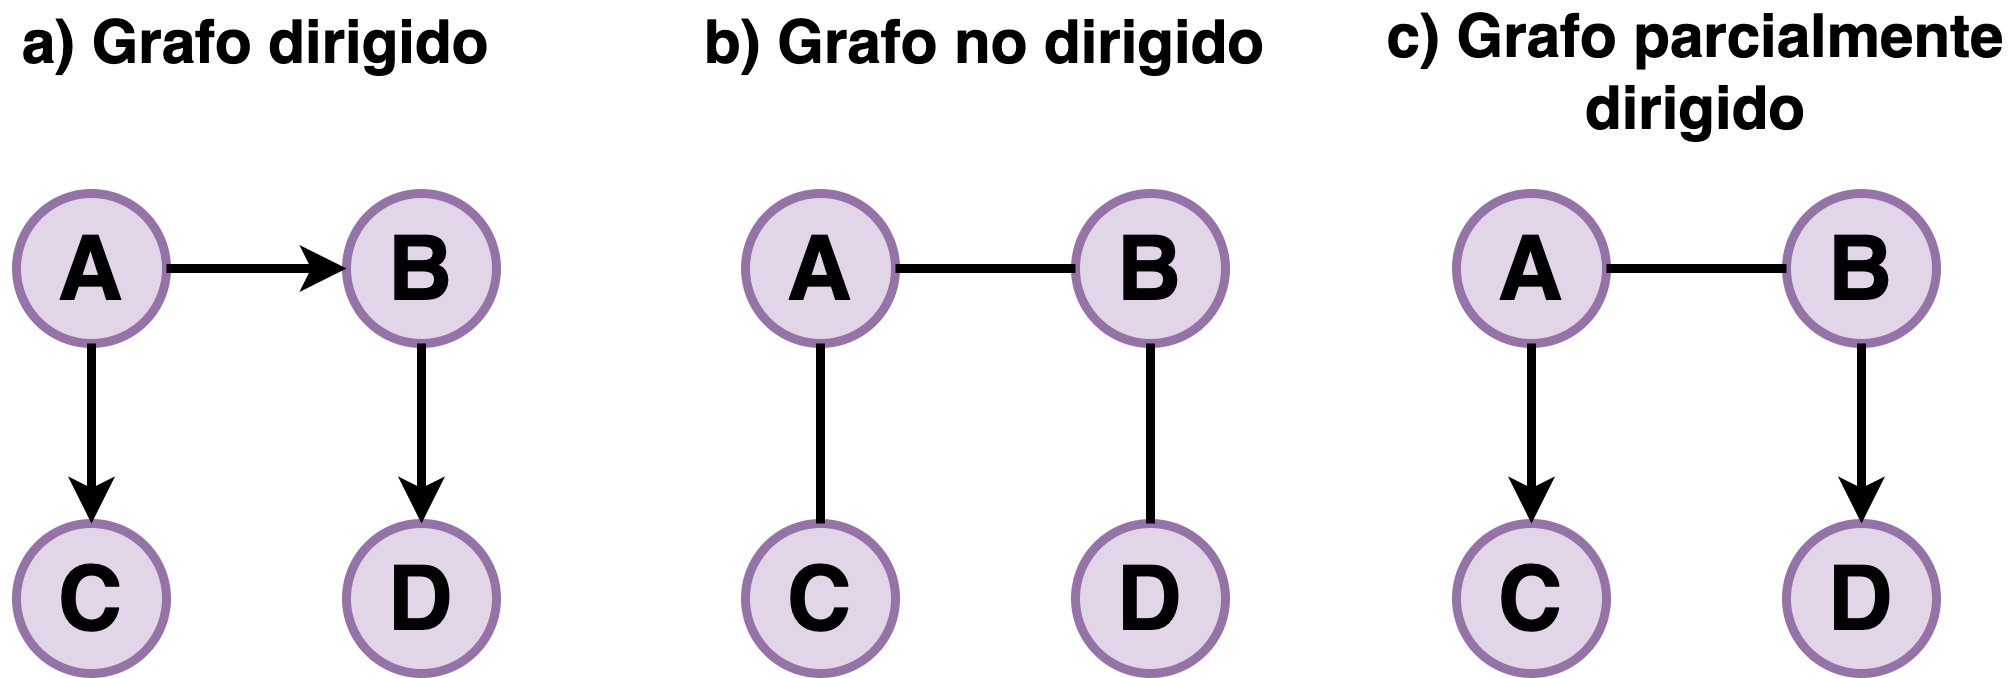
\includegraphics[scale=0.15]{figuras/fig1.png}
    % \caption[Así aparece el rótulo en el índice]{Así aparece el rótulo en el texto.}
    \caption[Tipos de grafos]{\textbf{Tipos de grafos.}}
    \label{fig1}
\end{figure}

La tabla~\ref{tab1} muestra...

\begin{table}[H]
    \centering
    \caption{Resumen de documentos y arquitecturas en el estado del arte}   
    \resizebox{0.95\textwidth}{!}{%
    \begin{tabular}{|p{2cm}|c|c|c|c|c|p{4.3cm}|p{5.6cm}|c|c|}
        \hline
        \rowcolor{gray!20} \textbf{Documento} & \textbf{CNN} & \textbf{VAE} & \textbf{GANs} & \textbf{Transformers} & \textbf{LSTM} & \textbf{Aplicación en la Música} & \textbf{Relevancia en el Estado del Arte} & \textbf{Simbólica} & \textbf{Audio} \\
        \hline
        \textbf{TFG Antonio Carpintero Castilla} & \ding{51} & \cellcolor{red!25} & \cellcolor{red!25} & \cellcolor{red!25} & \ding{51} & Generación de música Lo-Fi & Caso práctico en generación de un género específico & \ding{51} & \cellcolor{red!25} \\
        \hline
        \textbf{Estado del Arte - M72.1.09 Gestión y análisis de datos no estructurados} &  & \cellcolor{red!25} & \cellcolor{green!25}\ding{51} & \cellcolor{green!25}\ding{51} &  & Modelado de datos en entornos no estructurados & Explica el papel de Transformers en la IA musical & \ding{51} & \cellcolor{red!25} \\
        \hline
        \textbf{AI of Things (VI) - Inteligencia Artificial Generativa, creando música a ritmo de perceptrón} &  & \cellcolor{green!25}\ding{51} & \cellcolor{green!25}\ding{51} & \cellcolor{red!25} &  & Aplicación de modelos generativos en la música & Explica GANs y VAE en la síntesis musical & \ding{51} & \cellcolor{red!25} \\
        \hline
        \textbf{IA en la creatividad: Explorando la generación de arte y música} &  & \cellcolor{green!25}\ding{51} & \cellcolor{green!25}\ding{51} & \cellcolor{red!25} &  & Modelos generativos aplicados al arte y música & Justificación del impacto de la IA en la música &  & \cellcolor{green!25}\ding{51} \\
        \hline
        \textbf{A Transformer Generative Adversarial Network for Multi-Track Music Generation} &  & \cellcolor{red!25} & \cellcolor{green!25}\ding{51} & \cellcolor{green!25}\ding{51} &  & Generación de música polifónica multicanal & Combinación de Transformers y GANs para mejorar generación & \ding{51} & \cellcolor{red!25} \\
        \hline
        \hline
        \textbf{TFM} &  & \cellcolor{blue!25}\ding{51} & \cellcolor{blue!25}\ding{51} & \cellcolor{blue!25}\ding{51} &  & Generación de música personalizada & Justificación de modelos generativos en el TFM & & \cellcolor{blue!25}\ding{51} \\
        \hline
    \end{tabular}%
    }
    \label{tab1}
\end{table}

\subsection{Una subsubsección}
\label{una-subsubseccion}

El algoritmo~\ref{alg1} muestra...
\medskip

\begin{algorithm}[H]
\label{alg1}
\SetAlgoLined
\medskip
\begin{enumerate}
    \item Elegir una estructura de red $\mathcal{G}$ sobre $\mathbf{V}$, normalmente vacía. Establecer la puntuación máxima inicial: $Score_{max} = Score_{\mathcal{G}}$.
    \item Repetir los siguientes pasos mientras $Score_{max}$ siga aumentando:
    \begin{enumerate}
        \item Calcular las puntuaciones para todas las posibles redes modificadas $\mathcal{G}^{*}$ que se pueden obtener añadiendo, eliminando o reorientando un solo eje de $\mathcal{G}$ sin que se producan ciclos.
        \item Si para alguna de las redes modificadas $\mathcal{G}^{*}$ se cumple que $Score_{G^{*}} > Score_{\mathcal{G}}$, establecer $G = G^{*}$ y $Score_{max} = Score_{G^{*}}$.
    \end{enumerate}
    \item Devolver el DAG $\mathcal{G}$.
\end{enumerate}
 \caption{Algoritmo \textit{Hill-Climbing} (HC)}
\end{algorithm}


\newpage

Ejemplo de fórmula:

\begin{equation*}
    N_{k}(\mathbf{\mu},\mathbf{\Sigma}) = \frac{1}{\sqrt{2\pi\det(\Sigma})} \exp \bigg\{ -\frac{1}{2}(\mathbf{X}-\mathbf{\mu})^{T}\Sigma^{-1}(\mathbf{X}-\mathbf{\mu}) \bigg\} \quad \mathbf{X},\mathbf{\mu} \in \mathbb{R}^{k}
\end{equation*}

Otro ejemplo de fórmula:

\begin{equation*}
    \underbrace{P(\mathcal{B}|\mathcal{D}) = P(\mathcal{\mathcal{G}},\Theta|\mathcal{D})}_{\textbf{Aprendizaje}} = \underbrace{P(\mathcal{G}|\mathcal{D})}_{\textbf{Aprendizaje estructural}} \cdot \underbrace{P(\Theta|\mathcal{G},\mathcal{D})}_{\textbf{Aprendizaje paramétrico}}
\end{equation*}

%% OBJETIVOS

\cleardoublepage

\chapter{Objetivos}
\label{objetivos}

Describe aquí el objetivo general de tu Trabajo Fin de Máster y, a continuación, define los objetivos parciales:
\medskip
\begin{enumerate}[label=\destacado{\arabic*.}]
  \setlength\itemsep{1em}
  \item \textbf{Objetivo parcial 1.}

  \item \textbf{Objetivo parcial 2.}

  \item \textbf{Objetivo parcial 3.}
\end{enumerate}

%% METODOLOGÍA

\cleardoublepage

\chapter{Metodología}
\label{metodologia}

%% RESULTADOS Y DISCUSION 

\cleardoublepage

\chapter{Resultados y Discusión}
\label{resultados-y-discusion}

%% CONCLUSIONES

\chapter{Conclusiones}
\label{conclusiones}

\begin{enumerate}[label=\destacado{\arabic*.}]
  \setlength\itemsep{1em}
  \item Conclusión 1.

  \item Conclusión 2.

  \item Conclusión 3.
\end{enumerate}

%% LIMITACIONES Y PERSPECTIVAS DE FUTURO

\cleardoublepage

\chapter{Limitaciones y\\ Perspectivas de Futuro}
\label{limitaciones-y-futuro}


% INTRODUCCIÓN

\cleardoublepage

\chapter{Introducción}

Incluida en la clasificación de las bellas artes, en la lista propuesta por Ricciotto Canudo en su obra \emph{Manifiesto de las siete artes}, en la clasificación china de las tardes; y presente en cualquier obra audio visual contemporánea: cine, televisión, ``performances'', video juegos, ``video clips'', etc., la música es el elemento que marca una escena, condiciona una situación, acompaña una secuencia, potencia una acción, seduce a la audiencia, advierte al espectador o simplemente acompaña de fondo (y no por eso sin percibir menos atención) en la más mundana tarea como puede ser conducir un coche.

La música, en todos sus géneros formas, relata las costumbres de una región, de una nación, de un país, la moda de un determinado momento, se hace eco de hechos históricos y es capaz de transferir conocimiento y saber popular entre generaciones.

Es una manera de expresarse. Una forma de expresión que modifica la manera de sentir para seguir retroalimentando su presencia (quién no ha encontrado un patrón melódico en un llanto o en un ruido en plena calle).

La música, amplia, diversa e inmensa en número de piezas, consta de géneros musicales, que vienen a intentar clasificar y canonizar una composición musical, total o parcial, dentro de un grupo o conjunto, donde todos sus integrantes tengan rasgos comunes como: ritmo (compases y estructura), melodía, armonía, instrumentación, etc. En esencia, vienen a ser ``esas cosas que se perciben en conjunto y que hacen tipificar la pieza que se escucha''.

\section{Planteamiento del problema}

Tómese una serie de piezas musicales (cientos de ellas) y obténgase una representación computable de cada una. ¿Sería capaz una computadora de extraer patrones referenciales que permitieran clasificarlas? Esas clasificaciones: ¿se corresponderían con géneros musicales? ¿Cómo sabría la computadora de qué género musical se podría tratar en cada caso? Y si se añade una nueva pieza que concuerde levemente con alguna o algunas ya procesadas anteriormente, ¿será capaz de clasificarla? \textbf{¿Cómo aprende la máquina a distinguir géneros musicales?}

Esa es la gran pregunta que ha de hacerse para poder abordar la tarea de hacer un software que pueda clasificar piezas musicales.

... Y una vez clasificadas: \textbf{¿podría la máquina generar nuevas piezas musicales que se correspondan con un género conocido?}

Ese en concreto es el problema que se aborda en este trabajo de fin de máster. Para ello, se van a explorar distintas formas de abordar el problema, contraponiendo los resultados de unas y otras, y observando y evaluando qué alternativa cumple mejor con los requisitos planteados y cuál, además, aporta mejor gusto a la composición generada.


\section{Justificación}
La clasificación automática de géneros musicales aporta diversos valores. No se trata sólo de un desafío científico. También puede tener aplicaciones prácticas como:

\begin{itemize}
    \item \textbf{Sistemas de recomendación musical}: ser capaz de de clasificar de manera automática canciones por género es crucial para construir sistemas de recomendación por género.
    \item \textbf{Bibliotecas musicales}: agrupar un conjunto de piezas musicales por géneros aportaría la capacidad de poder obtener conjuntos basados características afines.
    \item \textbf{Análisis musicológico}: como herramienta para investigadores que necesiten estudiar la evolución de los géneros musicales. Analizar influencia de distintos factores en la aparición de un género musical, evolución y rasgos comunes, etc.
    \item \textbf{Educación musical}: ayudar a estudiantes a distinguir entre géneros musicales y aprender algunos nuevos, combinarlos entre ellos, etc.
\end{itemize}

En este ámbito, el ocio y entretenimiento no se han quedado fuera. La Inteligencia Artificial ha transformando la manera en que se crean, distribuyen y consumen contenidos:

\begin{itemize}
    \item Se proyecta que para 2025, la IA gestionará el 95\% de las experiencias de los clientes en el sector del entretenimiento, mejorando la personalización y la eficiencia en la interacción \cite{marketers}.
    
    \item El 15\% de las interacciones globales en servicios de atención al cliente estarán impulsadas por IA para 2025 \cite{marketers}.
    
    \item Plataformas como Netflix (con más de 232 millones de usuarios activos mensuales) utilizan IA para predecir el crecimiento de suscriptores y optimizar la calidad de transmisión \cite{marketers}.
    
    \item En el campo de la música, OpenAI ha desarrollado \textit{Jukebox}, una red neuronal capaz de generar música en distintos géneros, incluyendo voz y letra \cite{jukebox}.
    
    \item Según un informe de CISAC, la IA podría reducir los ingresos globales del sector musical y audiovisual en un 20\% y 25\% respectivamente para 2028 \cite{elpais}.
    
    \item En cine, tecnologías de IA han sido utilizadas para rejuvenecer digitalmente a actores, como en \textit{The Irishman} de Martin Scorsese \cite{linkedin}.
    
    \item En videojuegos, la IA permite adaptar dinámicamente la dificultad del juego, personalizando la experiencia del usuario \cite{iaespana}.
    
    \item En el deporte, se emplean algoritmos de IA para analizar datos de partidos anteriores, predecir resultados y optimizar estrategias \cite{learningheroes}.
\end{itemize}

Así, la Inteligencia Artificial también aporta nuevas formas de creatividad y personalización, replanteando el papel de los humanos en la creación cultural.

\section{Objetivos}
\label{objetivo-principal}
Desarrollar un programa basado en Inteligencia Artificial que sea capaz de generar música personalizada, utilizando métodos generativos adversariales, que pueda ser clasificada dentro de un género concreto.

Para desarrollar el objetivo general, han de alcanzarse los objetivos específicos:

\begin{enumerate}
    \item Recopilar ejemplos de \textbf{datos} correspondientes con piezas musicales representativas, de un género musical y que estén \textbf{bien etiquetadas}.
    
    \item Transformar esas piezas musicales en \textbf{estructuras de datos} analizables y computables.

    \item Diseñar un modelo basado en Inteligencia Artificial que sea capaz de \textbf{extraer información} crítica para \textbf{distinguir} cuáles son los \textbf{patrones} que asignan un pieza musical a un \textbf{género} concreto.

    \item Entrenar un modelo de Inteligencia Artificial, para que sea capaz de \textbf{generar} una pieza que sea reconocible como perteneciente a un género musical dado.

    \item \textbf{Evaluar} el modelo generador mediante métricas que se apliquen a los \textbf{datos de salida} generados.
\end{enumerate}

\section{Alcance}
Si se atiende al objetivo general, el alcance viene dado por la cantidad de géneros a seleccionar para poder producir piezas musicales distintas. (Una pieza musical vendrá dada por un género y un ruido aleatorio introducido de manera automática, aspecto este que limitaría el número máximo de piezas musicales distintas a producir por el sistema; es por eso que este ruido habrá de ser de gran dimensión).

\section{Estructura del documento}
Este documento se organiza de la siguiente manera:
\begin{itemize}
    \item \emph{Capítulo \textbf{1}}\textbf{: Introducción.} Presentación, exposición del problema y del trabajo que lo intenta resolver, justificación, objetivos, alcance y estructura (esta misma sección).
    \item \emph{Capítulo \textbf{2}}\textbf{: Estado del arte.} Revisión exhaustiva del estado del arte en el momento de acometer este trabajo fin de máster.
    \item \emph{Capítulo \textbf{3}}\textbf{: Marco teórico.} Exposición de los fundamentos teóricos en los que se basa este trabajo.
    \item \emph{Capítulo \textbf{4}}\textbf{: Métodos y Materiales.} Metodología utilizada y herramientas para llevar a cabo todo el proceso proyectual.
    \item \emph{Capítulo \textbf{5}}\textbf{: Resultados y Análisis.} Contraste de resultados y análisis de los mismos.
    \item \emph{Capítulo \textbf{6}}\textbf{: Conclusiones.} Presentación de conclusiones obtenidas del producto global del trabajo.
    \item \emph{Capítulo \textbf{7}}\textbf{: Limitaciones y perspectivas a futuro.} Propuestas de mejoras y líneas de expansión para futuros trabajos.
\end{itemize}
% ESTADO DEL ARTE

\cleardoublepage

\chapter{Estado del Arte}

Deténgase un momento antes de continuar. Piense en el concepto de Inteligencia Artificial en el más amplio espectro posible. Desde la más frívola de las presentaciones (por ejemplo: la inteligencia capaz de dominar el mundo en el universo de la saga de \emph{Terminator} o la Inteligencia Artificial capaz de generar recuerdos tan reales en tu cerebro de \emph{Desafío Total}), hasta la más estricta y formal de las definiciones, proporcionada en la asignatura \textbf{04-MIAR: Razonamiento Aproximado}:
\emph{``Sistema diseñado para funcionar con un cierto nivel de autonomía y que, basándose en datos de entradas proporcionadas por máquinas o por personas, infiere cómo lograr un conjunto de objetivos establecidos utilizando estrategias de aprendizaje automático o basadas en la lógica y el conocimiento, y genera información de salida, como contenidos Sistemas de inteligencia artificial generativos), predicciones, recomendaciones o decisiones, que influyan en los entornos con los que interactúa.''}

Ahora, vuelva a mirar a su alrededor, coja su teléfono móvil y haga cualquier consulta, regule las luces con el uso de su voz o pregunte a uno de los asistentes de voz que tenga a mano qué hora es y sea consciente de la tecnología que le rodea. El momento histórico que acontece ha permitido que anhelos del cine de los años 80 y 90, se basen en modelos matemáticos de la década de los 50 para que, con la potencia computacional de la segunda década de los 2000, sea capaz de empezar a vivirse en el día a día lo que antes era una utopía literaria.

Siguiendo la línea histórica, en el marco de las redes neuronales, en los años 80 empieza a aflorar el concepto \emph{Deep Learning}, sustentado en los algoritmos de retroprogragación de los pesos para la modulación y aprendizaje de una red neuronal.

Aún así, no son más potentes hoy en día las redes neuronales, de lo que lo eran entre las décadas de los 50 a 80, simplemente se ha propiciado el marco computacional, de cálculo y memoria, para ser manejadas de manera más precisa y con un tamaño creciente.

Y como si de un ecosistema vivo se tratara, el software que sustenta y ``da vida'' a los modelos matemáticos de \emph{Redes Neuronales}, han inferido en la creación, expansión y venta de hardware específico, como son los procesadores orientados a Inteligencia Artificial o la expansión de los procesadores gráficos, que por su arquitectura interna, son capaces de computar operaciones con matrices cada vez de mayor tamaño y cada vez más rápido.

Existe un completamente nuevo (no tiene más de 20 años) que no se puede pasar por alto: el concepto de \textbf{Big Data}. Con la explosión de las Bases de Datos en las décadas de los 70 y 80 del siglo pasado y la posterior consolidación de los Sistemas Gestores de Base de Datos, es en 2004 cuando Google presenta el concepto \emph{MapReduce}, como paradigma del manejo de información de manera paralela y distribuida. Esto, junto con el concepto \emph{IOT: Internet de las cosas} y la creación de sensores y captadores cada vez más livianos y parcos en consumo, ha provocado que la cantidad de datos, algunos de ellos etiquetados, agrupados en \emph{Datasets}, sea cada vez mayor y cuente con una diversidad temática nunca antes vista.

Así pues, un volumen y diversidad de datos cada vez mayor y una potencia de cálculo en consonancia, han dado lugar a mayores y mejores sistemas predictivos en muchos ámbitos, análisis de características en imágenes (Redes Neuronales Convolucionales), modelos de procesamiento del lenguaje natural (Transformers y LLMs), detección de anomalías en series temporales (modelos ARIMA, LSTMs), optimización de procesos industriales mediante mantenimiento predictivo, análisis de sentimientos en redes sociales, generación de contenido multimedia con IA generativa, mejora en la personalización de recomendaciones en plataformas digitales y simulaciones avanzadas en ciencias computacionales y biológicas.

Entre estos nuevos sistemas, están los incipientes modelos generativos, aparecidos a finales de la década de los años 90 del siglo pasado y principios de los 2000. Estos modelos son capaces de generar nuevo contenido, desarrollando cada vez un comportamiento más cercano al humano.

Aunque no sería hasta 2013 cuando apareciera el concepto \emph{VAE: Autoencoder Variacional} y 2014, cuando surgiera el concepto \emph{GAN: Red Generativa Adversarial}. Estos modelos, basados en \emph{Deep Learning}, proponen dos maneras de captar conocimiento a través del procesamiento de datos etiquetados.

\section{VAE: Variational Auto Encoders. Autoencode Variacional}

Según viene regocido en el artículo ``Autoencoding variational bayes''\citep{kingma2013vae}, los \emph{Autoencoders Variacionales} (VAE) han recorrido un largo camino desde su concepción hasta convertirse en una de las herramientas fundamentales en la generación de datos mediante inteligencia artificial. Desde su aparición, han sido una alternativa sólida a otros modelos generativos debido a su capacidad para estructurar representaciones latentes de manera probabilística, lo que ha permitido una mayor estabilidad en la generación y una mayor coherencia en la producción de datos sintéticos. Diseñados como una extensión de los autoencoder en su origen, los VAE cuentan con la diferencia clave de que en lugar de mapear cada entrada a un único punto en el espacio latente, lo hacen a una distribución probabilística. Esto permite una generación más controlada y variada. Esta innovación fue fundamental en áreas como la generación de imágenes y la modelización de secuencias temporales, donde la capacidad de interpolación y extrapolación de datos era esencial.

Conforme la investigación avanzó, los VAE comenzaron a adaptarse a nuevas aplicaciones, encontrando en la música un campo fértil para su desarrollo. La estructura musical, caracterizada por la interdependencia entre notas, acordes y estructuras melódicas, representó un desafío único para los modelos generativos. A diferencia de la generación de imágenes, donde la relación espacial entre píxeles es clave, en la música la relación entre eventos a lo largo del tiempo es lo que define la coherencia de una composición. Esto llevó a la combinación de VAE con otros enfoques como redes recurrentes y transformers, logrando modelos capaces de generar secuencias musicales con un sentido de continuidad más refinado. Uno de los avances más notables en este ámbito, fue publicado en el artículo científico ``A Hierarchical Latent Vector Model for Learning Long-Term Structure in Music''\citep{roberts2018musicvae}, desarrollado por \emph{Google Brain}, que introdujo un enfoque basado en aprendizaje latente para la interpolación y transformación de melodías.

La evolución de los VAE en la generación musical no se ha limitado únicamente a la síntesis de melodías, sino que también ha explorado la transformación estilística y la personalización de la música. Modelos recientes han incorporado mecanismos que permiten a los usuarios modificar atributos específicos de una pieza, como el tempo, la armonía o la instrumentación, generando variaciones a partir de un conjunto de datos inicial. Uno de los modelos más innovadores en este sentido es \emph{Jukebox}, desarrollado por OpenAI, que combina VAE con transformers para generar música con una calidad cercana a la de una composición humana.

A pesar de estos avances, los VAE aún presentan desafíos en la generación musical. Uno de los principales problemas ha sido la calidad del audio generado, ya que muchos modelos basados en VAE tienden a producir sonidos menos nítidos en comparación con otros enfoques como las Redes Generativas Adversariales (GANs). Sin embargo, investigaciones recientes han abordado este problema mediante la incorporación de técnicas híbridas que combinan la estabilidad de los VAE con la capacidad de refinamiento de las GANs, permitiendo una síntesis de audio más realista y detallada.

%En conclusión, los Autoencoders Variacionales han pasado de ser una curiosidad teórica a convertirse en una de las tecnologías más influyentes en el campo de la generación musical asistida por inteligencia artificial.%  ---> one of final conclusions

\section {GANS: Generative Adversarial Networks. Redes Generativas Adversariales.}

Según la famosa publicación de Ian GoodFellow: ``Generative adversarial networks''\citep{goodfellow2014gan} allá por 2014, hace poco más de 10 años, las \emph{Redes Generativas Adversariales} o \emph{GANs}, han revolucionado la generación de contenido en múltiples ámbitos, incluyendo la música. Estos modelos han demostrado que a veces, la rivalidad puede ser muy beneficiosa, si hace crecer a los contrincantes. Mientras que el generador intenta crear muestras cada vez más semejantes a los datos reales, el discriminador intentará distinguir entre las muestras generadas (falsas) y las reales. El generador tomará apunte de cuál es la distancia que el discriminador estableció entre sendas muestras, para intentar hacerlo mejor la próxima vez, lo que llevará a una mejora progresiva de la calidad del contenido generado. Esta dinámica ha permitido que las GANs sean aplicadas en la generación de imágenes, texto y, más recientemente, en la creación de música.

Inicialmente, la aplicación de las GANs en la música se encontró con desafíos significativos debido a la naturaleza estructurada y secuencial de la música. Para abordar esto, se desarrollaron variantes como \emph{MuseGAN}, introducida en 2018, que permitió la generación de música polifónica con múltiples instrumentos utilizando una arquitectura basada en redes convolucionales y recurrentes. MuseGAN fue un avance clave, ya que mostró que las GANs podían modelar estructuras musicales más complejas y generar composiciones que mantenían la cohesión armónica y rítmica.

Posteriormente, el campo avanzó con la introducción de \emph{C-RNN-GAN}, que combinaba redes recurrentes con GANs para generar secuencias musicales con coherencia temporal mejorada. Esta arquitectura permitió capturar mejor las dependencias a largo plazo en la música. Con el tiempo, se han desarrollado más modelos, como \emph{MidiNet}, que utilizó redes convolucionales para mejorar la calidad de las secuencias generadas en el dominio simbólico.

Uno de los enfoques más recientes en la generación musical mediante GANs ha sido la integración con \emph{Transformers}, lo que ha dado lugar a modelos como \emph{A Transformer Generative Adversarial Network for Multi-Track Music Generation}. Este modelo, basado en la estructura de atención de los Transformers, permite capturar relaciones a largo plazo entre diferentes pistas musicales, mejorando la calidad y la coherencia de la música generada.

Las GANs han transformado la forma en que se genera música mediante inteligencia artificial, permitiendo la síntesis de composiciones originales con una calidad cada vez mayor. Aunque aún existen desafíos técnicos, los avances en arquitectura y entrenamiento están allanando el camino para un futuro donde la IA pueda desempeñar un papel fundamental en la creatividad musical.

\section{Coherencia musical y memoria neuronal}

En el artículo ``Niveles de coherencia musical: la aportación de la música a la construcción de mundos''\citep{sibetrans2025coherencia} se hace mención a varios tipos de coherencia musical. En concreto, se expresa una de ellas como la \emph{\textbf{coherencia contextual}}: ``se refiere a la consideración de la pieza musical como unidad de sentido, como un universo en sí mismo.''

Es decir, estableciendo una analogía mundana, si cada pieza musical fuera un edificio en construcción, el cual se fuera construyendo mientras se escucha dicha pieza, \emph{no se podría poner el techo antes que los cimientos}. Es decir, imagínese una escala creciente de notas en una pieza musical en la que, de repente, los saltos entre notas sean diferentes y cuya progresión sea hacia arriba y hacia abajo. Esto daría lugar a incoherencia en lo que se esperaba en la pieza musical. De ahí que saber y recordar cuál fue la nota anterior (anteriores) es importante a la hora de componer y de almacenar información sobre música existente.

Así pues, las composiciones generadas por inteligencia artificial deben evitar la pérdida de estructura melódica y armónica, garantizando que la música no se perciba como una simple sucesión de notas sin conexión. Para abordar este problema, se ha trabajado en la integración de mecanismos que permitan capturar relaciones de largo plazo dentro de la música, asegurando que las redes neuronales generativas no solo reproduzcan patrones locales, sino que comprendan el contexto global de una pieza. 

El modelo que se propone en el artículo \textbf{``A Transformer Generative Adversarial Network for Multi-Track Music Generation''}\citep{jin2022transformer}, es una solución basada en el uso de \emph{self-attention}, una técnica que permite modelar dependencias a largo plazo dentro de la música polifónica. Este enfoque posibilita que el sistema aprenda la relación entre distintas voces o instrumentos, facilitando la sincronización entre líneas melódicas y estructuras rítmicas complejas. La integración de Transformers con GANs ha resultado ser una estrategia eficaz para reforzar la coherencia estructural, dado que los Transformers pueden procesar grandes secuencias de información de manera paralela, permitiendo que las decisiones de generación no estén limitadas a ventanas de tiempo cortas, como sucede en las arquitecturas recurrentes. 

Desde otra perspectiva, en la publicación \textbf{``Estado del Arte - M72.1.09 Gestión y análisis de datos no estructurados''}\citep{state_of_the_art2023} se enfatiza la importancia de los mecanismos de memoria en los modelos de generación musical. Tradicionalmente, las Redes Neuronales Recurrentes (RNN) y sus variantes como LSTM han sido utilizadas para modelar secuencias musicales, dado que son capaces de retener información de eventos pasados para influenciar la generación futura. Sin embargo, estas arquitecturas presentan problemas cuando se requiere mantener coherencia a lo largo de pasajes extensos. Los Transformers han emergido como una alternativa más robusta, al permitir que las relaciones entre eventos distantes sean capturadas de manera más eficiente, sin la necesidad de un procesamiento secuencial que limite la capacidad de memoria del modelo.

Uno de los retos en la generación musical es garantizar que los cambios en la melodía o armonía no sean abruptos ni carezcan de lógica interna. En este sentido, la combinación de GANs con Transformers introduce una mejora significativa en la modelización de estructuras globales. Mientras que las GANs se encargan de generar datos con alta fidelidad perceptual, los Transformers refuerzan la coherencia musical, asegurando que las transiciones entre secciones sean naturales y que la progresión armónica se mantenga fluida. Esta integración ha demostrado ser particularmente útil en la generación de música multicanal, donde la interacción entre instrumentos debe ser consistente y reflejar principios musicales bien establecidos.

Las investigaciones revisadas resaltan que la memoria neuronal y la coherencia musical son dos aspectos fundamentales en la evolución de los modelos generativos para la música. La capacidad de retener información a largo plazo y aplicar estos conocimientos en la generación de nuevas secuencias es lo que diferencia un modelo efectivo de uno que produce música carente de estructura. La aplicación de Transformers junto con GANs abre nuevas posibilidades en la generación de composiciones musicales que respeten la lógica interna de una obra, proporcionando un avance significativo en la inteligencia artificial aplicada a la creatividad musical.


\section{Explorando los ejemplos del estado del arte}

Las razones más relevantes a la hora de seleccionar los ejemplos de GANs y VAE del estado del arte, son su capacidad para modelar la generación de música con un alto nivel de coherencia estructural y estilística. Mientras que los VAE permiten la interpolación entre estilos musicales y la manipulación controlada de características latentes, las GANs han demostrado ser efectivas en la producción de música polifónica de calidad superior. La evolución de los modelos generativos en la música ha seguido un patrón de avance progresivo, impulsado por la necesidad de generar contenido coherente, expresivo y personalizado. A lo largo de los últimos años, se ha observado una convergencia entre distintas arquitecturas, desde modelos basados en representaciones probabilísticas como los \textbf{Autoencoders Variacionales (VAE)} hasta enfoques más sofisticados que emplean \textbf{Redes Generativas Adversariales (GANs) con Transformers}. Esta convergencia ha permitido superar limitaciones previas y expandir las posibilidades creativas en la composición automatizada.

La aplicación de los VAE en la generación musical ha sido ampliamente explorada, dado que estos modelos permiten interpolaciones estilísticas y modificaciones controladas de las piezas generadas. Su capacidad para capturar distribuciones latentes ha facilitado la transformación de obras musicales preexistentes, ajustando atributos específicos como el ritmo, la instrumentación y el timbre. En este sentido, la documentación revisada sobre el uso de los VAE en la generación musical ha sido clave para comprender cómo sistemas como \textbf{MusicVAE} han logrado avances en la manipulación de secuencias melódicas y en la exploración de nuevas combinaciones armónicas. La incorporación de documentos específicos ha permitido profundizar en la integración de técnicas probabilísticas para modelar atributos musicales, facilitando el diseño de estructuras latentes adaptadas a la composición automatizada.

El desarrollo de las \textbf{GANs} ha representado un hito en la generación de música con mayor realismo. La estructura competitiva entre generador y discriminador ha permitido alcanzar niveles superiores de fidelidad en la síntesis de melodías, armonías y ritmos, lo que se evidencia en trabajos como \textbf{``MuseGAN: Multi-track Sequential Generative Adversarial Networks for Symbolic Music Generation and Accompaniment''}\citep{dong2018musegan}, que han mostrado la capacidad de estas redes para producir música polifónica coherente, incorporando múltiples instrumentos en una misma composición. En este aspecto, la documentación revisada ha sido clave para entender el papel de las GANs en la generación de música, destacándose fuentes que describen la evolución de estas redes en su aplicación a la música multicanal. La información contenida en estos documentos ha sido esencial para comprender cómo la integración de mecanismos de autoatención en las GANs ha mejorado la coherencia armónica y la estructura rítmica, permitiendo la generación de piezas musicales más complejas y expresivas.

El impacto de los \textbf{Transformers en la generación musical} ha sido otro factor determinante en la evolución de los modelos generativos. Su capacidad para manejar relaciones de largo alcance en las secuencias ha permitido generar composiciones con una cohesión superior. La combinación de Transformers con GANs ha dado lugar a arquitecturas avanzadas que integran mecanismos de autoatención para modelar de manera efectiva la interacción entre distintos elementos musicales.

\newpage
A continuación, se enumeran los documentos utilizados y su justificación en el contexto del desarrollo del trabajo:

\begin{enumerate}
    \item \textbf{Estado del arte - M72.1.09 Gestión y análisis de datos no estructurados} \\ 
    Se ha utilizado para comprender las tendencias actuales en modelos generativos, especialmente en la evolución de arquitecturas basadas en \textbf{Transformers} y su impacto en la generación de contenido musical.

    \item \textbf{AI of Things (VI) - Inteligencia Artificial Generativa, creando música a ritmo de perceptrón} \\ 
    Documento clave para profundizar en la aplicación de \textbf{GANs y VAE en la síntesis musical}, detallando cómo estos modelos pueden ser utilizados para generar piezas de alta calidad y personalización.

    \item \textbf{A Transformer Generative Adversarial Network for Multi-Track Music Generation} \\ 
    Se ha empleado para comprender los enfoques más recientes que combinan \textbf{Transformers con GANs}, mostrando cómo la autoatención mejora la coherencia armónica y la estructura de la música generada.

    \item \textbf{TFG Antonio Carpintero Castilla} \\ 
    Aporta un caso de estudio relevante sobre la generación de música en un ámbito específico, como el género \textbf{Lo-Fi}, permitiendo analizar la adaptación de modelos generativos a estilos concretos.

    \item \textbf{Attributes-Aware Deep Music Transformation} \\ 
    Se ha utilizado para entender la transformación musical basada en modelos generativos, explorando cómo las técnicas de modelado latente pueden modificar atributos específicos sin alterar la estructura de una composición.
\end{enumerate}

Estos documentos han permitido construir una visión integral sobre el estado actual de la generación de música mediante inteligencia artificial, aportando conocimientos clave sobre las arquitecturas más avanzadas y sus aplicaciones en la composición automatizada.

\renewcommand{\arraystretch}{1.3} % Espaciado vertical en filas

\begin{table}[H]
    \centering
    \caption{Resumen de documentos y arquitecturas en el estado del arte}   
    \resizebox{0.95\textwidth}{!}{%
    \begin{tabular}{|p{2cm}|c|c|c|c|c|p{4.3cm}|p{5.6cm}|c|c|}
        \hline
        \rowcolor{gray!20} \textbf{Documento} & \textbf{CNN} & \textbf{VAE} & \textbf{GANs} & \textbf{Transformers} & \textbf{LSTM} & \textbf{Aplicación en la Música} & \textbf{Relevancia en el Estado del Arte} & \textbf{Simbólica} & \textbf{Audio} \\
        \hline
        \textbf{TFG Antonio Carpintero Castilla} & \ding{51} & \cellcolor{red!25} & \cellcolor{red!25} & \cellcolor{red!25} & \ding{51} & Generación de música Lo-Fi & Caso práctico en generación de un género específico & \ding{51} & \cellcolor{red!25} \\
        \hline
        \textbf{Estado del Arte - M72.1.09 Gestión y análisis de datos no estructurados} &  & \cellcolor{red!25} & \cellcolor{green!25}\ding{51} & \cellcolor{green!25}\ding{51} &  & Modelado de datos en entornos no estructurados & Explica el papel de Transformers en la IA musical & \ding{51} & \cellcolor{red!25} \\
        \hline
        \textbf{AI of Things (VI) - Inteligencia Artificial Generativa, creando música a ritmo de perceptrón} &  & \cellcolor{green!25}\ding{51} & \cellcolor{green!25}\ding{51} & \cellcolor{red!25} &  & Aplicación de modelos generativos en la música & Explica GANs y VAE en la síntesis musical & \ding{51} & \cellcolor{red!25} \\
        \hline
        \textbf{IA en la creatividad: Explorando la generación de arte y música} &  & \cellcolor{green!25}\ding{51} & \cellcolor{green!25}\ding{51} & \cellcolor{red!25} &  & Modelos generativos aplicados al arte y música & Justificación del impacto de la IA en la música &  & \cellcolor{green!25}\ding{51} \\
        \hline
        \textbf{A Transformer Generative Adversarial Network for Multi-Track Music Generation} &  & \cellcolor{red!25} & \cellcolor{green!25}\ding{51} & \cellcolor{green!25}\ding{51} &  & Generación de música polifónica multicanal & Combinación de Transformers y GANs para mejorar generación & \ding{51} & \cellcolor{red!25} \\
        \hline
        \hline
        \textbf{TFM} &  & \cellcolor{blue!25}\ding{51} & \cellcolor{blue!25}\ding{51} & \cellcolor{blue!25}\ding{51} &  & Generación de música personalizada & Justificación de modelos generativos en el TFM & & \cellcolor{blue!25}\ding{51} \\
        \hline
    \end{tabular}%
    }
    \label{tab1}
\end{table}

Como se puede contemplar en la tabla \ref{tab1} los requerimientos establecidos en este TFM (última fila con celdas en color azul) no se llegan a satisfacer por completo por ningún trabajo previo. Si bien, hay que remarcar dos de entre todos ellos.

En este trabajo se intentará establecer una comparativa entre soluciones basadas en los dos tipos de arquitectura: VAE y GANs. Por lo que, cogidos de uno en uno:

\begin{table}[H]
    \centering
    \caption{Recuperado de la tabla \emph{Resumen de documentos y arquitecturas en el estado del arte}~\ref{tab1}. Ejemplo que más criterios cumple usando arquitectura VAE.}
    \resizebox{0.95\textwidth}{!}{%
    \begin{tabular}{|p{2cm}|c|c|c|c|c|p{4.3cm}|p{5.6cm}|c|c|}
        \hline
        \rowcolor{gray!20} \textbf{Documento} & \textbf{CNN} & \textbf{VAE} & \textbf{GANs} & \textbf{Transformers} & \textbf{LSTM} & \textbf{Aplicación en la Música} & \textbf{Relevancia en el Estado del Arte} & \textbf{Simbólica} & \textbf{Audio} \\
        \hline
        \textbf{IA en la creatividad: Explorando la generación de arte y música} &  & \cellcolor{green!25}\ding{51} & \cellcolor{green!25}\ding{51} & \cellcolor{red!25} &  & Modelos generativos aplicados al arte y música & Justificación del impacto de la IA en la música &  & \cellcolor{green!25}\ding{51} \\
        \hline
    \end{tabular}%
    }
    \label{tab2}
\end{table}

Si se trata de hacer un modelo basado en redes VAE, \textbf{IA en la creatividad: Explorando la generación de arte y música} es un buen ejemplo del que partir y en el que apoyarse, como se ve en el fragmento de tabla \ref{tab2}.

\begin{table}[H]
    \centering
    \caption{Recuperado de la tabla \emph{Resumen de documentos y arquitecturas en el estado del arte}~\ref{tab1}. Ejemplo que más criterios cumple usando arquitectura GANs.}
    \resizebox{0.95\textwidth}{!}{%
    \begin{tabular}{|p{2cm}|c|c|c|c|c|p{4.3cm}|p{5.6cm}|c|c|}
        \hline
        \rowcolor{gray!20} \textbf{Documento} & \textbf{CNN} & \textbf{VAE} & \textbf{GANs} & \textbf{Transformers} & \textbf{LSTM} & \textbf{Aplicación en la Música} & \textbf{Relevancia en el Estado del Arte} & \textbf{Simbólica} & \textbf{Audio} \\
        \hline
        \textbf{A Transformer Generative Adversarial Network for Multi-Track Music Generation} &  & \cellcolor{red!25} & \cellcolor{green!25}\ding{51} & \cellcolor{green!25}\ding{51} &  & Generación de música polifónica multicanal & Combinación de Transformers y GANs para mejorar generación & \ding{51} & \cellcolor{red!25} \\
        \hline
    \end{tabular}%
    }
    \label{tab3}
\end{table}

Por el contrario, si se trata de mezclar redes GAN con el uso de Transformers para mantener la coherencia, el ejemplo más representativo puede ser \textbf{A Transformer Generative Adversarial Network for Multi-Track Music Generation}, representado en el fragmento de tabla \ref{tab3}.

Si bien no se enfocó al uso de generación de música audible, dada la minuciosidad de la explicación, la extensión y el uso de imágenes como refuerzo de las explicaciones. Didácticamente hablando, es un documento ejemplar.




% MARCO TEÓRICO

\cleardoublepage

\chapter{Marco teórico}

En este capítulo se va a profundizar en la teoría que sustenta la generación de contenidos y dentro de ello, la generación musical. Para que el lector no tenga que dar nada por sentado, se va a hacer un repaso desde la generación del sonido, captación, transformación, codificación y guardado, hasta la aprehensión de conocimiento por parte de un sistema de Inteligencia Artificial y la posterior generación de nuevo conocimiento, completando así el círculo que se dejó abierto en los pasos previos de codificación, donde se tenían datos, hasta llegar transformarlos y obtener información a partir de ellos, para después poder generar nuevas piezas musicales.

\section{Del sonido a los bytes: proceso de captación, transformación y discretización}

\subsection{La naturaleza del Sonido}
El sonido es una onda mecánica que se propaga a través de un medio elástico, como el aire, el agua o un cuerpo sólido. El sonido se genera cuando un objeto vibra, haciendo que las moléculas del medio se agiten alrededor de su posición de reposo. Esto forma perturbaciones en forma de ondas longitudinales. La figura \ref{fig:onda_sonora} muestra un diagrama de cómo se produce este fenómeno y el patrón de perturbación longitudinal que produce.

\begin{figure}[H]
  \centering
  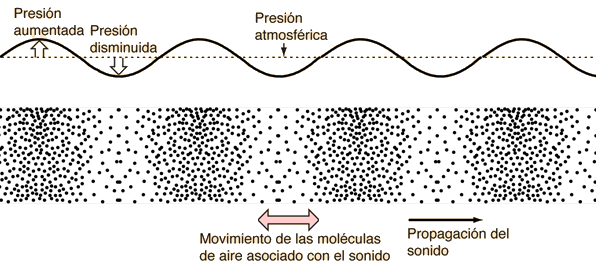
\includegraphics[width=0.9\textwidth]{images/wave.png}
  \caption{Onda sonora.}
  \label{fig:onda_sonora}
\end{figure}

Las propiedades principales del sonido son:

\subsubsection{Frecuencia ($f$)}
Determina el tono de un sonido. Se define como:
\begin{equation}
    f = \frac{1}{T}
\end{equation}
donde $T$ es el período de la onda en segundos. En términos de la velocidad de propagación $v$ y la longitud de onda $\lambda$, la frecuencia también puede expresarse como:
\begin{equation}
    f = \frac{v}{\lambda}
\end{equation}

Se mide en Hertz (Hz). Una mayor frecuencia corresponde a sonidos más agudos, mientras que una menor frecuencia genera sonidos más graves. El oído humano puede detectar frecuencias en el rango de 20 Hz a 20 kHz.

\subsubsection{Amplitud ($A$)}
La amplitud es la máxima elongación de la onda respecto a su posición de equilibrio. Está relacionada con la intensidad del sonido percibido.
\begin{equation}
    I = 10 \log_{10} \left( \frac{P}{P_0} \right)
\end{equation}
donde $P$ es la potencia de la onda sonora y $P_0$ es la potencia de referencia estándar (normalmente $10^{-12}$ W/m$^2$ en aire).

Se mide en decibelios (dB). Los sonidos de mayor amplitud se perciben como más fuertes; por el contrario, los de menor amplitud son más suaves.

\subsubsection{Longitud de onda ($\lambda$)}
La longitud de onda es la distancia entre dos puntos consecutivos en fase (por ejemplo, de cresta a cresta) y está dada por:
\begin{equation}
    \lambda = \frac{v}{f}
\end{equation}

En medios distintos del aire, la longitud de onda varía debido a cambios en la velocidad de propagación. Por ejemplo, en el agua, donde el sonido viaja a aproximadamente 1482 m/s, la misma frecuencia produce una longitud de onda mayor que en el aire.

\subsubsection{Velocidad de propagación ($v$)}
La velocidad del sonido depende del medio a través del cual se propaga y se determina mediante:
\begin{equation}
    v = \sqrt{\frac{B}{\rho}}
\end{equation}
donde $B$ es el módulo de elasticidad del medio y $\rho$ su densidad.

En distintos medios, la velocidad del sonido varía significativamente:
\begin{itemize}
    \item Aire (20$^\circ$C): 343 m/s
    \item Agua: 1482 m/s
    \item Acero: 5960 m/s
\end{itemize}

\subsubsection{Presión sonora ($p$)}
El sonido también puede describirse en términos de presión acústica, relacionada con la intensidad de la onda por:
\begin{equation}
    I = \frac{p^2}{\rho v}
\end{equation}

Esta presión es responsable de cómo percibimos el volumen del sonido. Se mide en Pascales (Pa).

\subsubsection{Intensidad del sonido ($I$)}
La intensidad del sonido mide la cantidad de energía que transporta una onda sonora por unidad de área y se expresa como:
\begin{equation}
    I = \frac{P}{A}
\end{equation}

\subsubsection{Amplitud ($A$) e Intensidad ($I$)}
La amplitud es la máxima elongación de la onda respecto a su posición de equilibrio. Está relacionada con la intensidad del sonido percibido, que se mide en decibeles (dB) y se expresa como:
\begin{equation}
    I = 10 \log_{10} \left( \frac{P}{P_0} \right)
\end{equation}
donde $P$ es la potencia de la onda sonora y $P_0$ es la potencia de referencia estándar (normalmente $10^{-12}$ W/m$^2$ en aire).

Sonidos de mayor amplitud se perciben como más fuertes, mientras que los de menor amplitud son más suaves.

\begin{tcolorbox}[title=Relación entre Amplitud e Intensidad,colback=gray!10, colframe=gray!50, sharp corners=south]
La amplitud representa la variación de presión en el medio por efecto de la onda sonora. La intensidad sonora, en cambio, está relacionada con la percepción subjetiva del volumen. Aunque están correlacionadas, la percepción auditiva del volumen no es lineal respecto a la amplitud. Se rige en una escala logarítmica.\vspace{10pt}

\parbox{\textwidth}{\textbf{Cómo percibe el oído los cambios de amplitud e intensidad}}
El sistema auditivo humano no responde de manera proporcional a los cambios en la amplitud de las ondas sonoras.

Un sonido de doble de amplitud no se percibe como ``el doble de fuerte''. Para que un sonido se perciba ``el doble de fuerte'', su intensidad debe aumentar aproximadamente 10 veces. Cada incremento de 10 dB en intensidad se siente como un sonido aproximadamente el doble de fuerte.

El oído humano es más sensible a ciertos rangos de frecuencia, lo que significa que los cambios de amplitud pueden percibirse de manera distinta según la frecuencia del sonido. Por ejemplo, contando con la misma amplitud, sonidos de 1000 Hz son percibidos con mayor intensidad que sonidos de 100 Hz.\vspace{10pt}

\parbox{\textwidth}{\textbf{Ejemplos de percepción de cambios de amplitud, intensidad y ambos}}
\begin{itemize}
    \item \emph{Cambio de amplitud}: golpear un tambor con más fuerza produce un sonido más fuerte sin cambiar su tonalidad (se mantiene la frecuencia).
    \item \emph{Cambio de intensidad}: Aumentar el volumen de una radio mantiene la misma música pero a un nivel sonoro más alto.
    \item \emph{Cambio de ambos}: un grito, que comienza como un susurro y termina en un grito fuerte, no solo varía en amplitud, sino que también cambia en intensidad progresivamente.
\end{itemize}

Los cambios en amplitud pueden detectarse más fácilmente en sonidos de corta duración o con transiciones bruscas, como golpes de tambor o explosiones, mientras que cambios en intensidad pueden ser más notorios en sonidos sostenidos.

Este comportamiento explica por qué los ajustes de volumen en dispositivos de audio son exponenciales en lugar de lineales.
\end{tcolorbox}

\subsubsection{Timbre}
El timbre es la característica del sonido que permite diferenciar dos sonidos de igual frecuencia y amplitud, que son generados por fuentes diferentes. Está determinado por la composición espectral de la onda sonora, es decir, la combinación de frecuencias fundamentales y armónicas presentes en el sonido. Matemáticamente, se representa como la suma de ondas sinusoidales:
\begin{equation}
    S(t) = \sum_{i=1}^{n}n A_i \cos(\omega_i t)
\end{equation}
donde cada término representa un armónico con su propia amplitud y frecuencia.

El timbre es un elemento clave y central en la música y en la percepción del habla, pues es la propiedad que hace único el sonido de cada instrumento o la voz de una persona.

\subsection{Captura del Sonido}
Para digitalizar el sonido, primero es necesario \textbf{capturarlo} utilizando un transductor, que convierte la energía acústica, en forma de vibraciones en el medio, en una señal eléctrica. Estos dispositivos pueden ser, por ejemplo:

\begin{itemize}
    \item \textbf{Micrófonos}: capturan ondas de sonido y las convierten en señales eléctricas.
    \item \textbf{Pastillas de guitarra}: detectan vibraciones de las cuerdas y las transforman en corriente eléctrica.
    \item \textbf{Sensores piezoeléctricos}: utilizados en pianos eléctricos y otros instrumentos electrónicos.
\end{itemize}

La señal eléctrica obtenida sigue siendo analógica y debe ser convertida en una representación digital mediante un convertidor \emph{Analógico-Digital \textbf{(A/D)}}.

\subsection{Muestreo}
El sonido en su forma natural es una \textbf{onda analógica}, lo que significa que tiene una variabilidad infinita en el tiempo y la amplitud. Sin embargo, las computadoras y dispositivos digitales solo pueden manejar información en forma de números discretos. Para convertir una señal analógica en digital, es necesario \textbf{tomar muestras} de la amplitud del sonido en distintos instantes de tiempo.

Este proceso se asemeja a tomar fotografías de una escena en movimiento a una tasa constante: cuanto mayor sea la cantidad de fotos por segundo (tasa de muestreo), más suave y precisa será la representación de la escena.

\section{Frecuencia de Muestreo}

La \textbf{frecuencia de muestreo} determina cuántas veces por segundo se toma una muestra de la señal de audio. Se mide en \textbf{Hertz (Hz)} y sigue el \textbf{Teorema de Nyquist-Shannon}, que establece que la frecuencia de muestreo debe ser al menos \textbf{el doble de la frecuencia más alta contenida en la señal original}:

\begin{equation}
    f_s \geq 2 f_{max}
\end{equation}

donde:
\begin{itemize}
    \item $f_s$ es la frecuencia de muestreo.
    \item $f_{max}$ es la frecuencia más alta en la señal de entrada.
\end{itemize}

Si este criterio no se cumple, se produce \textbf{aliasing}, un efecto en el que las frecuencias más altas se distorsionan y terminan representándose incorrectamente en el audio digital.

Ejemplo de \textbf{frecuencias de muestreo comunes}:
\begin{itemize}
    \item \textbf{44.1 kHz}: usado para codificar sonido en CD de audio. Permite captar frecuencias hasta \textbf{22.05 kHz}.
    \item \textbf{48 kHz}: utilizado en audio para video y grabaciones estándar.
    \item \textbf{96-192 kHz}: aplicado en grabaciones de alta fidelidad y producción de estudio.
\end{itemize}

\subsection{Cuantización: Representación Numérica de las Muestras}

Cada muestra tomada en el proceso de muestreo debe convertirse en un valor numérico finito. Este proceso se llama \textbf{cuantización}, y su precisión depende de la \textbf{profundidad de bits}.

Ejemplos de resoluciones comunes:
\begin{itemize}
    \item \textbf{8 bits} – 256 niveles posibles (baja calidad, usada en telefonía).
    \item \textbf{16 bits} – 65,536 niveles (calidad estándar de CD).
    \item \textbf{24 bits} – 16,777,216 niveles (grabaciones profesionales).
\end{itemize}

Cuanto mayor es la profundidad de bits, menor es el \textbf{ruido de cuantización}, que es la diferencia entre la señal original y su versión cuantizada.

\subsection{Alias y pérdida de información}

Si la frecuencia de muestreo es demasiado baja, se produce un fenómeno llamado \textbf{aliasing}, en el cual las frecuencias más altas aparecen distorsionadas y se confunden con frecuencias más bajas.

Para evitar esto, se utilizan \textbf{filtros antialiasing} antes de la digitalización, que eliminan las frecuencias superiores a la mitad de la frecuencia de muestreo.

Ejemplo:
\begin{itemize}
    \item Si se digitaliza una señal con \textbf{una frecuencia de muestreo de 20 kHz}, pero la señal contiene componentes de hasta \textbf{30 kHz}, estas frecuencias más altas se distorsionarán.
\end{itemize}

\subsection{Aplicaciones del Muestreo}

\begin{table}[H]
    \centering
    \caption{Frecuencia de muestreo y profundidad de bits según la aplicación.}
    \begin{tabular}{|l|c|c|}
        \hline
        \textbf{Aplicación} & \textbf{Frecuencia de Muestreo} & \textbf{Profundidad de Bits} \\
        \hline
        \textbf{Telefonía digital} & 8 kHz & 8 bits \\
        \textbf{Radio FM} & 32 kHz & 12 bits \\
        \textbf{CD de audio} & 44.1 kHz & 16 bits \\
        \textbf{Grabaciones de estudio} & 96-192 kHz & 24 bits \\
        \hline
    \end{tabular}
    \label{tabla:frecuencia_muestreo}
\end{table}

La tabla \emph{Frecuencia de muestreo y profundidad de bits según la aplicación} \ref{tabla:frecuencia_muestreo} muestra una tabla comparativa de usos, frecuencias de muestreo y profundidad (o anchura) de bits utilizados en su representación digital.

\subsection{Percepción Auditiva y Frecuencia de Muestreo}

El oído humano tiene una respuesta no lineal a las frecuencias y la amplitud del sonido. Aunque el rango audible se encuentra entre \textbf{20 Hz y 20 kHz}, la sensibilidad es mayor en el rango de \textbf{1 kHz a 5 kHz}, donde se encuentra la mayor parte del contenido del habla.

\subsection{Reconstrucción del Sonido Digitalizado}

Después de la digitalización, el sonido debe convertirse nuevamente en una señal analógica para ser escuchado. Esto se realiza mediante un \textbf{convertidor digital-analógico (DAC)}, que:
\begin{enumerate}
    \item \textbf{Interpola} los valores entre muestras para suavizar la transición.
    \item \textbf{Usa un filtro de reconstrucción} para eliminar artefactos digitales.
    \item \textbf{Produce una señal analógica continua} para su reproducción.
\end{enumerate}

\section{MP3: un formato reducido}

El formato MP3 marcó un antes y un después en la digitalización del sonido. Fue el vehículo que revolucionó el consumo de música, popularizando el formato de audio digital, combinando eficiencia de compresión y facilidad de reproducción con \emph{códecs}. Dio nombre a pequeños aparatos que durante la primera década de los años 2000 inundaron bolsillos, dando la posibilidad de tener varios discos de música en el mismo espacio que un llavero. Fue, sin saberlo, el vehículo que abrió la puerta a la piratería y a la compartición ilícita de ficheros.

\subsection{Codificación y formatos de audio}

Una vez que la señal de audio ha sido muestreada y cuantificada, es necesario almacenarla en un formato digital adecuado. Para ello, los datos obtenidos son organizados en estructuras llamadas \textbf{códecs} (codificador/decodificador), que definen cómo se comprimen y guardan los archivos de audio.

Los formatos de audio digital pueden dividirse en tres grandes categorías:

\begin{enumerate}
    \item \textbf{Formatos sin compresión}: Guardan la señal tal cual fue capturada, sin ninguna reducción de datos. Ejemplos:
    \begin{itemize}
        \item \textbf{PCM} (Pulse Code Modulation): base de todos los formatos sin compresión.
        \item \textbf{WAV} (Waveform Audio File Format): utilizado en entornos profesionales por su fidelidad.
        \item \textbf{AIFF} (Audio Interchange File Format): equivalente de WAV para sistemas Mac.
    \end{itemize}
    
    \item \textbf{Formatos comprimidos sin pérdida}: Reducen el tamaño del archivo sin eliminar información del sonido original. Ejemplos:
    \begin{itemize}
        \item \textbf{FLAC} (Free Lossless Audio Codec): muy popular en audiófilos y distribución digital de alta calidad.
        \item \textbf{ALAC} (Apple Lossless Audio Codec): alternativa de Apple al FLAC.
        \item \textbf{APE} (Monkey’s Audio): menos común, pero con tasas de compresión más altas.
    \end{itemize}

    \item \textbf{Formatos comprimidos con pérdida}: fruto de algoritmos de compresión perceptual, el tamaño ha sido reducido al máximo exponente posible, eliminando partes de la señal consideradas inaudibles. Ejemplos:
    \begin{itemize}
        \item \textbf{MP3} (MPEG-1 Audio Layer III): el más famoso y extendido.
        \item \textbf{AAC} (Advanced Audio Codec): formato utilizado en iTunes, YouTube y Spotify, con mejor calidad que MP3 al mismo nivel de \emph{bitrate}.
        \item \textbf{OGG Vorbis}: alternativa libre con mejor calidad que MP3, usada en videojuegos y streaming.
    \end{itemize}
\end{enumerate}

\section{Bitrate: Definición y su impacto en la calidad del MP3}

Antes de continuar, es necesario aclarar un concepto clave en la codificación eficiente y correcta de música en MP3.

\subsection{¿Qué es el bitrate?}
El \textbf{bitrate} es la tasa cantidad de datos en un segundo del fichero de audio. Se mide en \textbf{kilobits por segundo (kbps)} y determina la calidad y el tamño del fichero de la siguiente manera:
\begin{itemize}
    \item \textbf{Bitrate alto}: mayor calidad de audio y ficheros de mayor tamaño.
    \item \textbf{Bitrate bajo}: menor calidad y archivos más pequeños.
\end{itemize}

\subsection{Bitrates más comunes en MP3 y su calidad percibida}
El MP3 permite codificar audio en diferentes bitrates, cada uno con una calidad de sonido distinta.

\begin{table}[H]
    \centering
    \caption{Comparación de bitrates y calidad de sonido en el formato MP3.}
    \resizebox{\textwidth}{!}{%
    \begin{tabular}{|c|l|l|}
        \hline
        \textbf{Bitrate (kbps)} & \textbf{Calidad percibida} & \textbf{Uso típico} \\
        \hline
        320 kbps  & Casi idéntico al original & Audio de alta calidad, producción musical \\
        256 kbps  & Excelente calidad, mínima pérdida & Descargas de alta fidelidad, iTunes \\
        192 kbps  & Buena calidad, ligera pérdida & Streaming de alta calidad, radio online \\
        160 kbps  & Calidad aceptable & Spotify estándar, radio digital \\
        128 kbps  & Pérdida de detalles en frecuencias altas & Antiguas descargas MP3, radio FM \\
        96 kbps   & Pérdida notable, sonido más plano & Podcasts, audiolibros \\
        64 kbps   & Baja calidad, sonido metálico & Streaming de voz, radio de baja calidad \\
        32 kbps o menos & Calidad muy pobre, muchas pérdidas & Uso extremo en redes con bajo ancho de banda \\
        \hline
    \end{tabular}
    }
    \label{tab:bitrates}
\end{table}

En la tabla \emph{Comparación de bitrates y calidad de sonido en el formato MP3}\ref{tab:bitrates} se recogen los valores más comunes.

\subsection{¿Cuál es un bitrate adecuado?}
El bitrate óptimo depende del uso específico y del balance entre calidad y tamaño del archivo:

\begin{itemize}
    \item Para \textbf{escuchar música con buena calidad}, un bitrate de 192 kbps es un buen punto intermedio.
    \item Para \textbf{calidad similar a la de un CD}, se recomienda 320 kbps en formato MP3.
    \item Para \textbf{streaming}, los servicios más utilizados emplean tasas variables:
    \begin{itemize}
        \item \textbf{Spotify}: 96 kbps (básico), 160 kbps (normal), 320 kbps (premium).
        \item \textbf{YouTube Music}: Dependiendo de la conexión, varía entre 48 kbps y 256 kbps en AAC.
    \end{itemize}
\end{itemize}

\subsection{Efectos de un bitrate bajo en la calidad del audio}
La compresión MP3 reduce el tamaño del archivo eliminando datos considerados menos perceptibles para el oído humano. Sin embargo, si el bitrate es demasiado bajo, ocurre que:

\begin{enumerate}
    \item Se eliminan demasiadas \textbf{frecuencias altas}, reduciendo la claridad del sonido.
    \item Aparecen \textbf{artefactos de compresión} (ruidos metálicos, eco, distorsión).
    \item Se pierde \textbf{profundidad y riqueza sonora}, dando una sensación de audio plano.
\end{enumerate}

Bitrates menores de 128 kbps producen diferencias, con el audio original, audibles en reproductores más básicos, afectando la experiencia de escucha.

\subsubsection{MP3: Compresión perceptual y revolución digital}

El formato \textbf{MP3} (MPEG-1 Audio Layer III) se convirtió en el estándar de facto para la música digital gracias a su gran capacidad de reducción del tamaño de los archivos, sin una pérdida de calidad perceptible en \emph{bitrates} determinados.

\subsubsection{Ventajas del MP3}
\begin{itemize}
    \item \textbf{Alta eficiencia en almacenamiento}: Un archivo MP3 puede ser hasta \textbf{10 veces más pequeño} que su equivalente en WAV sin comprimir.
    \item \textbf{Compatibilidad universal}: Es reproducible en prácticamente cualquier dispositivo, desde teléfonos móviles hasta sistemas de sonido profesionales.
    \item \textbf{Facilidad de distribución}: Su tamaño reducido lo hizo ideal para la difusión de música en Internet, dando lugar a plataformas como Napster en los 2000 y posteriormente al auge del streaming.
\end{itemize}

\subsubsection{Desventajas del MP3}
\begin{itemize}
    \item \textbf{Pérdida de calidad}: A bitrates bajos (como 128 kbps), pueden aparecer artefactos sonoros y pérdida de claridad en frecuencias altas.
    \item \textbf{Formatos más eficientes lo han superado}: Actualmente, códecs como \textbf{AAC, Opus y FLAC} han reemplazado al MP3 en muchas plataformas de streaming y almacenamiento de alta calidad.
\end{itemize}

%\subsection{Impacto del MP3 en la industria musical}
%El MP3 cambió para siempre la forma en que se consume la música. Su aparición permitió la popularización de la música digital, pero también trajo consigo desafíos para la industria:

%\begin{itemize}
%    \item \textbf{Explosión de la piratería}: La facilidad de compartir archivos MP3 a través de Internet llevó a la creación de plataformas como \textbf{Napster}, lo que causó una crisis en la industria discográfica.
%    \item \textbf{Cambio en los modelos de negocio}: Las disqueras tuvieron que adaptarse al formato digital, dando paso a servicios como \textbf{iTunes, Spotify y Apple Music}.
%    \item \textbf{Transición hacia el streaming}: Con el aumento de la velocidad de Internet, el almacenamiento local de archivos MP3 ha disminuido en favor de la transmisión en tiempo real.
%\end{itemize}

\section{De los datos a la información}

La información no es más que datos con significado. Partiendo de esta idea, los datos se podrían enunciar como la unidad mínima que compone la información, una vez estos son interpretados.

Para ello, es necesario tratarlos, guardarlos, manejarlos correctamente, transformarlos... en esencia, adecuarlos para extraer toda la información posible.


\subsection{Tratamiento de los datos}
\label{tratamiento-datos}

Para el entrenamiento de los modelos basados en Inteligencia Artificial que se plantearán para cumplir los objetivos, se van a utilizar 3 extensos datasets, cuyo tamaño y diversidad de géneros musicales contenidos abran posibilidad de poder obtener una herramienta que tenga un desempeño a la altura de lo que se podría esperar.

Asi pues, los 3 datasets propuestos son:

\begin{itemize}
    \item \textbf{FMA (Free Music Archive) Dataset}
        Las pistas se encuentran en formato \emph{MP3}, existiendo hasta tres variantes de tamaño del conjunto de datos.
        Se incluyen metadatos como título, artista, álbum, y etiquetas de género.
    \item \textbf{Million Song Dataset}
        Contiene 1500 ficheros en formato \emph{MP3}, distribuidos en 15 categorías de género. Es un dataset que se puede nutrir de servicios como Spotify y Last.fm.
    \item \textbf{MTG-Jamendo Dataset}
       Cuenta con más de 50,000 pistas y 190 géneros, distribuidos en ficheros \emph{MP3}. Los metaadatos están descritos en etiquetas de géneros musicales, instrumentos, emociones y temas.
\end{itemize}
En la sección \textbf{Materiales - Datos}\ref{materiales-datos} del siguiente capítulo, se puede consultar información mucho más detallada de cada una de estas tres fuentes de datos que se van a utilizar.

\subsection{Aprendiendo sobre géneros musicales}

Según la \emph{Real Academia Española} (RAE), \emph{aprender} se define como ``adquirir el conocimiento de algo por medio del estudio o de la experiencia''\citep{rae_aprender}. Entiéndase el estudio como ese ejercicio mental para llegar a esos conocimientos. Pero el estudio, planteado así, es algo inherente al humano. Ni siquiera los animales tendrían la capacidad de estudiar. Cuanto menos, una máquina.

Por lo tanto, la única manera que tendría una ordenador de aprender sería \emph{adquirir experiencia}. De la misma manera que un ratón de laboratorio, durante múltiples experimentos, puede ir recordando, \emph{amoldando} sus \emph{recuerdos} con los eventos que van aconteciendo, en el aprendizaje profundo o \emph{Deep Learning}, la estructura de red neuronal que va haciéndose eco de esos cambios que se van sucediendo, se convierte en una herramienta poderosísima para el análisis y clasificación de datos complejos, incluida la música y las pautas que la describen. 

Este tipo de aprendizaje permite a los modelos identificar patrones ocultos y aprender características específicas de distintos géneros, de la misma manera que lo haría un oyente que nunca ha escuchado música antes y que carece de conocimientos musicales: oyendo \emph{miles de veces cientos de canciones distintas} o lo que es lo mismo: explorando grandes conjuntos de datos \emph{etiquetados} (de alguna manera).

Una de las formas de realizar este análisis es el uso de redes neuronales convolucionales (\emph{Convolutional Neural Networks}, CNN) junto con algún mecanismo que implemente \emph{memoria recurrente} para dicha red, como por ejemplo los (\emph{Long Short-Term Memory}, LSTM). Basadas en el reconocimiento de imágnenes, este tipo de redes han supuesto un antes y un después en la visión (y aprehensión visual) por computadora. Una de las características más llamativas de este tipo de redes es la arquitectura \emph{hardware} sobre la que se suele apoyar: usa la \emph{GPU} en vez del procesador central de la máquina, dada la naturaleza matricial de la representación de los datos en imágenes.

Pero si la música es sonido, ¿cómo puede una \emph{CNN} analizar audio?: extrayendo la representación espectral del sonido o espectrograma y analizando una imagen del mismo; a su vez, las LSTM manejarían secuencias temporales de datos musicales, permitiendo modelar la continuidad y dependencia entre las notas.

En este trabajo se van a abordar dos maneras equivalente de hacer esto, teniendo en cuenta las últimas tendencias en Inteligencia Artificial.

\subsection{Variational Autoencoders (VAE)}

Los \textbf{Autoencoders} son redes neuronales diseñadas para aprender una representación codificada y ``comprimida'' de los datos de entrada, con el fin de ser reconstruidos cometiendo el menor error posible. Esto es, en definitiva, \textbf{aprender las características esenciales de los datos} y cofificarlas \textbf{en un espacio de menor dimensión.}

La figura \ref{fig:vae} ilustra cómo sería la arquitectura base.

\begin{figure}[H]
  \centering
  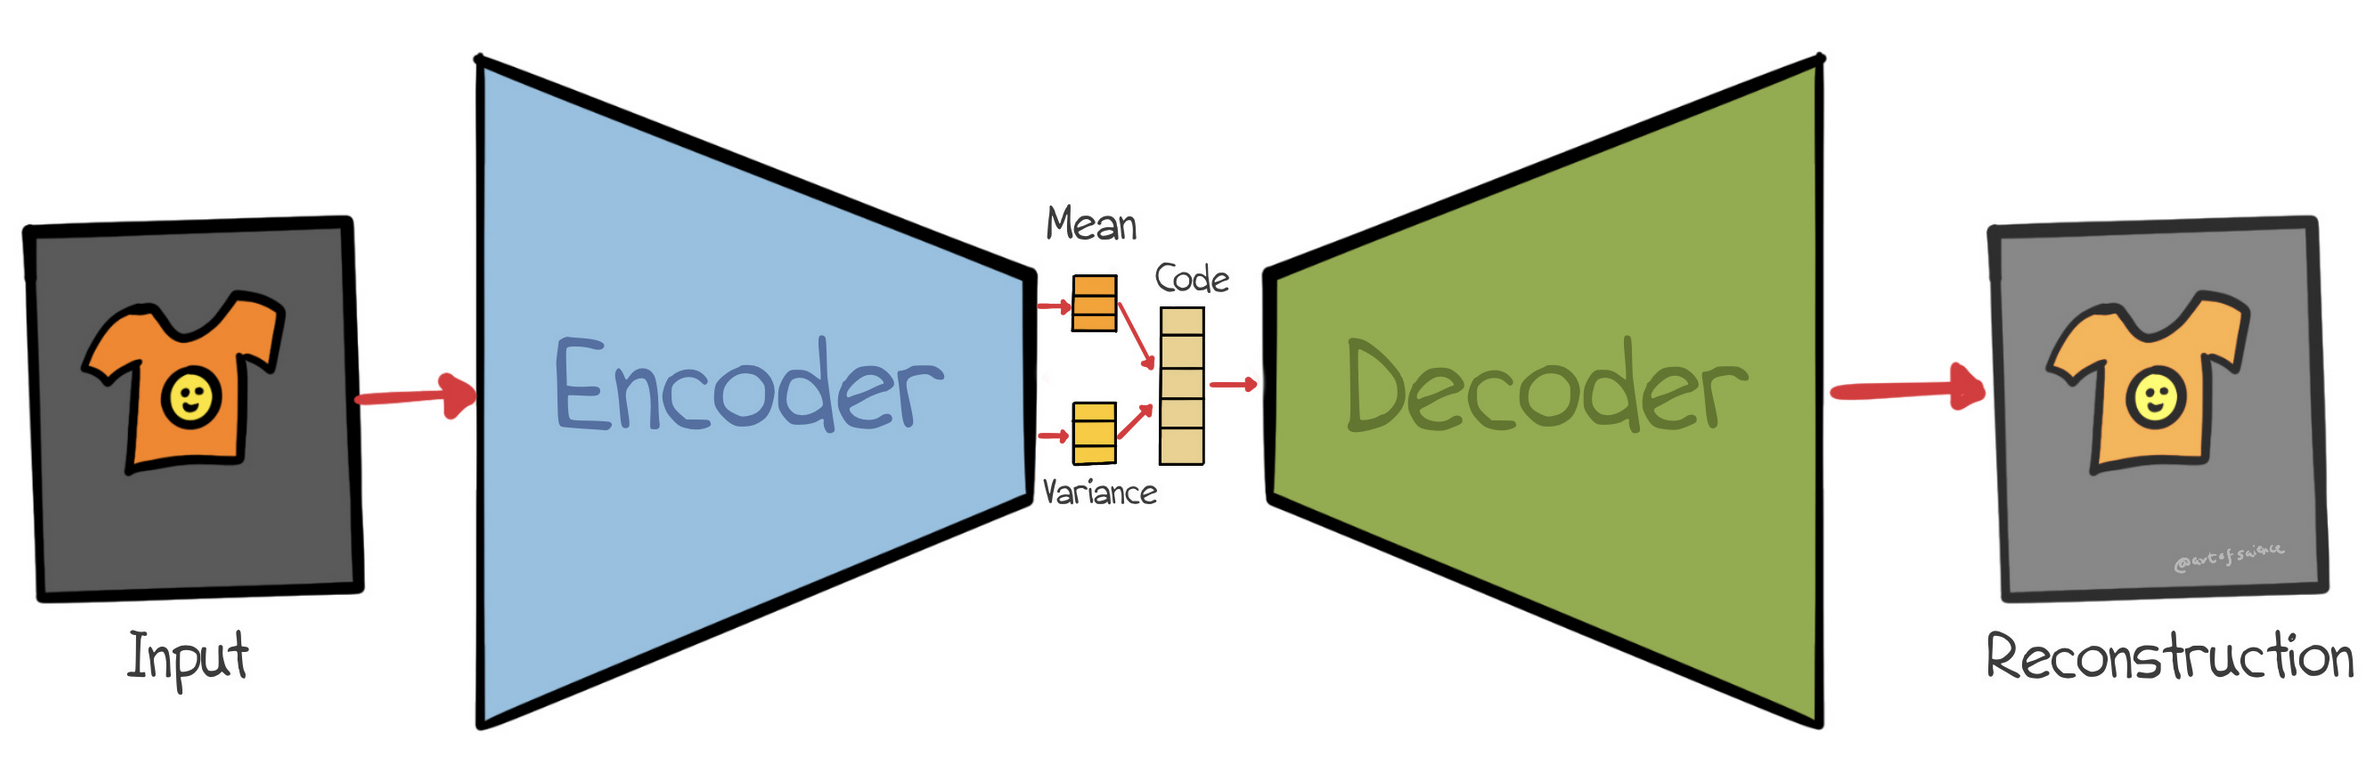
\includegraphics[width=0.9\textwidth]{images/vae.png}
  \caption{Variational Autoencoder.}
  \label{fig:vae}
\end{figure}

Ésta se compone de:

\begin{enumerate}
    \item \textbf{Codificador (Encoder)}: transforma la entrada original en una representación comprimida de menor dimensión.
    \item \textbf{Espacio latente}: representación interna de los datos. Albergará las caractarísticas principales de los datos usando una menor dimensión. Es el alma del autoencoder.
    \item \textbf{Decodificador (Decoder)}: reconstruye la entrada original (o lo intenta) a partir de la representación de los datos en el espacio latente.
\end{enumerate}


Haciendo un símil, al igual que cuando una persona cuenta un chiste y otra lo escucha para poder volverlo a contar, el receptor no retiene todos los detalles de la historia, sólo necesita recordar \textbf{la esencia de la gracia}, para volver a \emph{contar el chiste} de nuevo.

El entrenamiento de estas redes busca minimizar una \textbf{función de pérdida de reconstrucción}, que marcará la la diferencia entre la entrada original y la reconstrucción: entrada y salida del autoencoder; se puede utilizar, por ejemplo, el \emph{Mean Square Error} (MSE):

\begin{equation}
    L(x, \hat{x}) = \| x - \hat{x} \|^2
\end{equation}

Donde \( x \) es la entrada original y \( \hat{x} \) la salida reconstruida por el decodificador.

Uno de los problemas que presenta este modelo es que el espacio latente no está ordenado. Es decir: no se atiene a unas normas o reglas en las que la información esté estructurada o cuya ordenación tenga algún significado. Simplemente se han ido almacenando datos y serán utilizados para la fase de decodificación (generación).

Además de esto, disponen de una \emph{baja variabilidad generativa}, pues están diseñados para saber \emph{reproducir la entrada} solamente. Esto también llevará a un sobreajuste de la red.

Para paliar estas limitaciones, aparece la idea de \textbf{Autoencoders Variacionales (VAE)}. Enfocando todos los esfuerzos en dar un orden al espacio latente, en vez de mapear una entrada a un punto específico, los VAE introducen un enfoque probabilístico en dicho espacio, mapeando cada entrada a una \textbf{distribución probabilística \textbf{multivarinate}} en el espacio latente, ofreciendo una mayor variabilidad y capacidad generativa.

Estos nuevos y más sofisticados  autoencoders,\textbf{VAE}, dada su representación de datos en el espacio latente de manera probabilística, representan una herramienta muy útil en la captura y comprensión de características en datos complejos, pues no sólo ``comprimen'' la información, sino que son capaces de capturar estructuras inherentes y distribuciones subyacentes en el espacio de datos (relaciones que en principio no se conocían entre los datos).

De manera análoga, las tres fases de funcionamiento de este nuevo modelo son:

\begin{enumerate}
    \item \textbf{Codificación probabilística}: se asigna cada entrada a una distribución Gaussiana en el espacio latente.
    \item \textbf{Muestreo del espacio latente}: el muestreo desde esta distribución permite la generación de múltiples versiones ``cercanas'' al dato original.
    \item \textbf{Decodificación estocástica}: se reconstruyen las características del dato de entrada a partir de muestras del espacio latente.
\end{enumerate}

Una vez visto esto, la pregunta es: ¿cómo entonces hará un VAE para codificar ficheros \emph{MP3}?

\subsubsection{Procesamiento previo de los datos: de MP3 a números}
\label{proc_mp3}
Los archivos \textbf{MP3} necesitarán un preprocesado para convertir la señal de audio en un formato adecuado para que el VAE, modelo matemático y computable, pueda trabajar con ellos.

El camino a seguir desde el fichero de audio hasta convertirse en datos en el espacio latente conlleva las siguientes fases:

\begin{enumerate}
    \item \textbf{De música en \emph{MP3} a números} \\
    El primer paso es \emph{decodificar el archivo MP3} y convertir la señal de audio a un \emph{array} de valores numéricos que represente el sonido a lo largo del tiempo. Para reducir la dimensionalidad total de la muestra y poderla manejar en piezas más pequeñas, se aplican técnicas de ventana deslizante y la extracción del espectrograma de cada fragmento del archivo, utilizando la Transformada de Fourier de Ventana Corta (STFT):
    \[
        X(t, f) = \sum_{n=0}^{N-1} x(n)w(n-t)e^{-j2\pi fn/N},
    \]
    donde $X(t, f)$ representa el espectrograma del fragmento de audio, $x(n)$ es la señal de entrada, y $w(n)$ es una ventana de análisis.

    \begin{figure}[H]
      \centering
      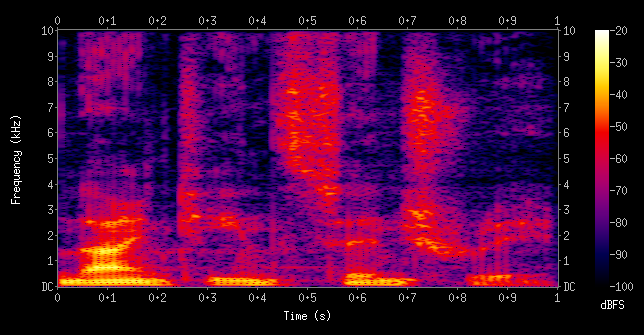
\includegraphics[width=0.85\textwidth]{images/espectrograma.png}
      \caption{Espectrograma}
      \label{fig:espectrograma}
    \end{figure}

    \item \textbf{Representación Espectral (Espectrograma)} \\
    El resultado del STFT es un \emph{espectrograma}, como el que se ve en la figura \ref{fig:espectrograma}, el cual muestra cómo cambia la energía de las distintas frecuencias a lo largo del tiempo. Este espectrograma puede interpretarse como una \emph{imagen} (tratable con una \emph{CNN} tal y como se ha descrito anteriomente), donde las filas representan las frecuencias y las columnas el tiempo.

    \item \textbf{Normalización y Entrada al VAE} \\
    El espectrograma se normaliza para que sus valores estén en un rango definido y se pasa como entrada al VAE. El \emph{codificador} del VAE ``aprenderá'' a comprimir y guardar esta representación en el \emph{espacio latente probabilístico}, asignando cada dato a una distribución Gaussiana multivariante.

    \item \textbf{Representación Latente} \\
    La representación latente captura las \emph{características principales} de la señal de audio: tono, textura del sonido, dinámica temporal... en un espacio mucho más reducido y estructurado, donde será posible \emph{muestrear y obtener nuevas variaciones del sonido}.
\end{enumerate}

Este tipo de autoencoders también podrían utilizarse para:
\begin{itemize}
    \item \textbf{Interpolación de Estilos}: los VAE pueden \emph{combinar estilos musicales distintos}, capturando las transiciones entre ellos y generando nuevos híbridos.
    \item \textbf{Personalización de Características}: permiten modificar atributos específicos, como el tempo, la armonía o la instrumentación, adaptando una pieza musical a las preferencias del usuario.
    \item \textbf{Captura de Coherencia Temporal}: en combinación con redes recurrentes, los VAE mejoran la continuidad temporal de secuencias complejas.
\end{itemize}

\subsection{GANs - Transformers}

Se propone al lector repasar el concepto de \href{https://es.wikipedia.org/wiki/Prueba_de_Turing}{Test de Turing}. Como si de pasar uno de estos test se tratara, existe un modelo de tipo generativo, es decir, diseñado para crear contenido nuevo, que se basa en la \emph{dialéctica} entre sus dos componentes, en la que una de ellas intentará hacer creer a la otra, de ahí la analogía con el test anteriomente citado, que lo que está ``viendo'' no se trata de contenido generado, sino de contenido original.

Las \textbf{GANs (Generative Adversarial Networks)} son unos modelos basados en redes neuronales, diseñados para aprender las características de un conjunto de datos a través de un proceso competitivo, adversarial, entre dos redes: \textit{generador} y \textit{discriminador}. Su capacidad para modelar distribuciones complejas las convierte en herramientas poderosas para captar patrones y relaciones latentes.

\begin{figure}[H]
  \centering
  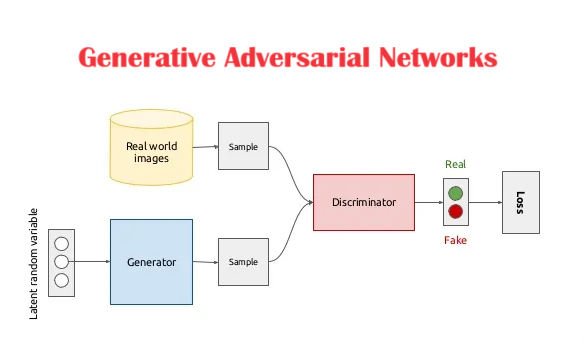
\includegraphics[width=0.8\textwidth]{images/gan.png}
  \caption{GANs (Generative Adversarial Networks)}
  \label{fig:gan}
\end{figure}

La figura \ref{fig:gan} muestra la estructura interna básica de este tipo de modelos, los cuáles se componen de dos elementos básicos:

\begin{itemize}
    \item \textbf{Discriminador (D):} tiene como cometido diferenciar entre datos reales y generados.
    \item \textbf{Generador (G):} su objetivo es generar datos que sean indistinguibles de los datos reales.
\end{itemize}

El entrenamiento de estas dos redes es muy distinto:
\begin{enumerate}
    \item Se entrena el discriminador a parte, con datos reales, los cuáles será capaz de reconocer con un error mínimo.
    \item El generador se entrena produciendo datos a partir de ruido aleatorio. Parte de de una red en principio sin entrenar, que irá variando sus pesos internos, con la diferencia que el discriminador devuelva de comparar (con respecto a la realidad que él sí conoce, dada por la \emph{función de pérdida}) entre cada muestra generada y los datos reales. De esta manera, el discriminador irá haciendo de ``crítico'' en la evaluación de la generación, hasta que el generador consiga engañarlo.
\end{enumerate}

\subsubsection{Transformers y memoria}

Los \textbf{Transformers} son un modelo de Inteligencia Artificial que han revolucionado el campo del aprendizaje secuencial, gracias a su mecanismo de \textit{autoatención}, son capaces de capturar relaciones entre las posiciones de la secuencia de manera paralela, pudiendo así aprender relaciones complejas, en el tiempo y entrenar modelos de mayor tamaño y más eficaces, en menos tiempo. La capacidad para capturar dependencias a largo plazo es lo que las hace tan distintas y valiosas, postulándose como idóneas para la aprehensión de características en \textbf{secuencias de datos (temporales) como texto y audio}.

Introducido por \textbf{Vaswani et al. (2017)} en el artículo \textit{Attention is All You Need}, los Transformers han revolucionando el procesamiento de lenguaje natural (NLP), la visión por computadora, música y generación de texto.

\begin{figure}[H]
  \centering
  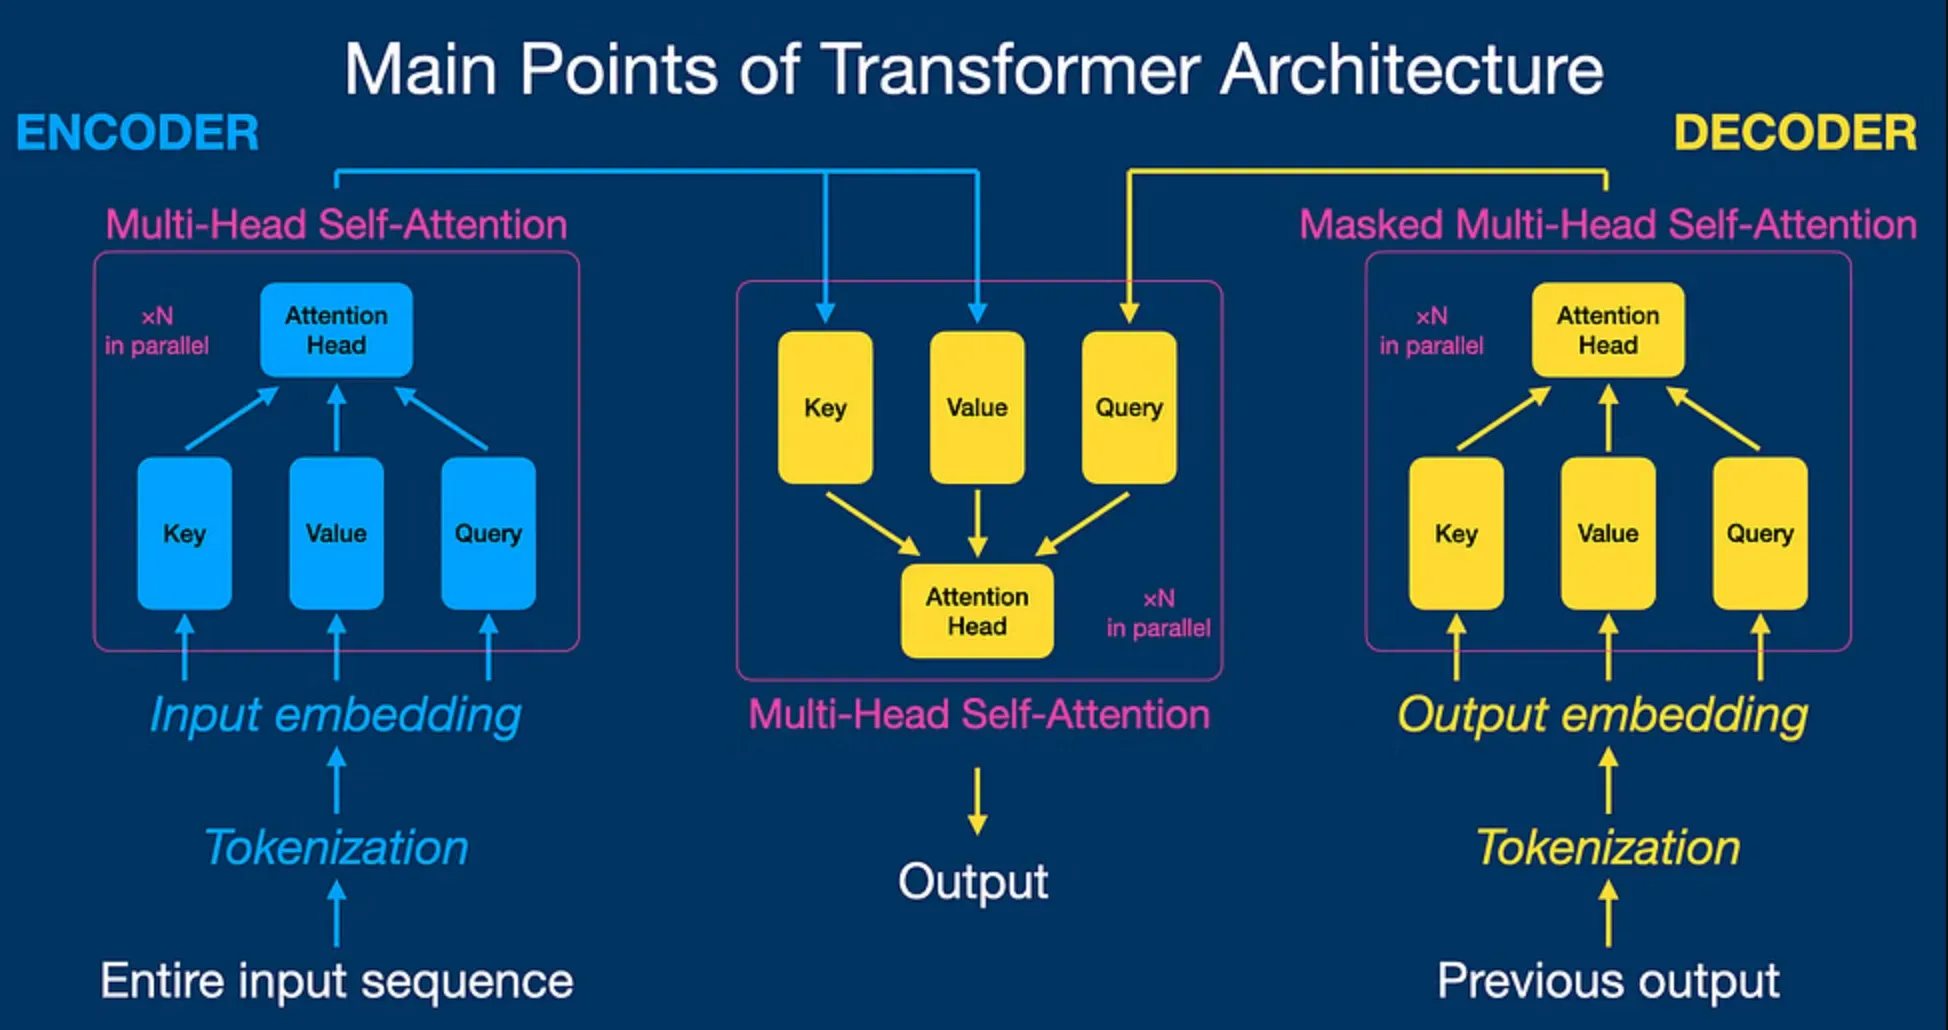
\includegraphics[width=1\textwidth]{images/transformer.png}
  \caption{Transformer Architecture}
  \label{fig:transformer}
\end{figure}

Como queda representado en la figura \ref{fig:transformer}, la arquitectura Transformer consta de \textbf{dos bloques principales}: el \textit{codificador (encoder)} y el \textit{decodificador (decoder)}. Estos trabajan en conjunto para convertir una secuencia de entrada en una secuencia de salida.

El \textbf{encoder} tiene como objetivo aprender una representación interna de la entrada, preservando las relaciones entre todos los elementos de la secuencia. Está compuesto por:
\begin{itemize}
    \item \textbf{Módulo de Autoatención (Self-Attention):} evalúa la importancia relativa de cada elemento en relación con los demás.
    \item \textbf{Red Feed-forward:} una red neuronal densa que transforma la salida del módulo de autoatención.
\end{itemize}

Cada capa encoder contiene:
\begin{enumerate}
    \item \textit{Autoatención multicanal (Multi-Head Self-Attention).}
    \item \textit{Capa normalizadora y red feed-forward.}
    \item \textit{Sumas residuales para estabilizar el aprendizaje.}
\end{enumerate}

Por su parte, el \textbf{decoder} genera la secuencia de salida basándose en las representaciones aprendidas por el codificador. Sus principales componentes incluyen:
\begin{itemize}
    \item \textbf{Atención enmascarada (Masked Attention):} bloquea las posiciones futuras en la secuencia para garantizar que no se utilice información no disponible.
    \item \textbf{Atención cruzada (Cross-Attention):} permite que el decodificador se enfoque en las partes relevantes de la secuencia de entrada.
\end{itemize}

El \textbf{mecanismo de autoatención} es el núcleo del Transformer y la clave de su éxito: \textbf{evalúa la importancia relativa entre todos los elementos de la secuencia simultáneamente.} Para saber más, sobre este complejo proceso, no dude en consultar el enlace ``Transformer Architecture '' de ``BotPenguin''\cite{botpenguin2025}.

El entrenamiento del Transformer tiene como finalidad minimizar una función de pérdida \emph{(cross entropy loss)} entre la secuencia generada y la secuencia esperada.

\begin{tcolorbox}[title=Silbar es cosa de niños,colback=gray!10, colframe=gray!50, sharp corners=south]

Un gesto tan sencillo y mundano como silbar, puede ilustrar lo que se intenta subsanar con el uso de Transformers.

Un silbido para llamar a alguien, persona o animal, puede ser un sonido simple, exhalado con fuerza, con un tono y una intensidad definidos.

Pero quién no ha visto sometido alguna vez a una melodía pegadiza, que se ha colado en el subconsciente y se repite mañana, tarde y noche en la cabeza. El impulso de silbarla en algún momento es incontenible.

Y ahí puede venir el problema de la coherencia, incluso para los silbadores más avezados, pues un simple cambio en una nota hará tener que recordar otra vez la secuencia de nuevo y volver a empezar a silbar.

De eso se encargaría el Transformer, de que las notas sucesivamente, una tras otra, sean cocherentes y tengan sentido.

Seguro que ha escuchado alguna vez y/o conoce y recuerda el tema principal de la banda sonora ``La muerte tiene un precio'', un \emph{Western} clásico protagonizado por \emph{Clint EastWood}. Este podría ser un ejemplo de cómo algo sencillo y mundano, como un silbido, aunque no lo parezca, requiere destreza, entrenamiento, rigos musical y coherencia, resultando ser algo mucho más laborioso de lo que en principio pudo parecer.

\end{tcolorbox}

\subsubsection{Métodos Combinados (GANs + Transformers)}

La combinación de estos dos modelos, \textit{GANs} y \textit{Transformers}, bien articulados, serían capaces de obtener tanto \textbf{relaciones locales} (GANs) como \textbf{dependencias en el tiempo a largo plazo} (Transformers); esta dupla se presenta como una solución perfecta a la hora de recordar patrones musicales dentro de géneros y ser capaces de reproducirlos.

Pero, \textbf{¿cómo se combinan y articulan estos dos modelos?} Pues ni más ni menos que incorporando la \textbf{arquitectura Transformer en el generador de la GAN}, tal y como se hizo en el antecedente revisado en el estado del arte ``A Transformer Generative Adversarial Network for Multi‐Track Music Generation''\citep{jin2022transformer}.

Así, el proceso de entrenamiento, combina procesos y objetivos de entrenamiento adversarial (GAN) y aprendizaje secuencial (Transformer). El proceso se divide en varias fases.

\paragraph{1º.- Pre-tratamiento de los datos.} 

El tratamiento previo de las pistas \emph{MP3} será el mismo que se ha descrito para VAE en el punto \ref{proc_mp3}.

\paragraph{2º.- Preentrenamiento de la GAN. El Discriminador.} 

Este proceso puede comenzar por el entrenamiento del Discriminador con muestras reales. Si bien no se trata de un paso obligatorio puede reportar beneficios a corto plazo durante el entrenamiento del Generador, como:

\begin{itemize}
    \item El generador al principio produce muestras de ruido aleatorio puro, lo que puede confundir al discriminador. De esta manera, se minimizaría.
    \item Proporciona una base sólida para que el discriminador entienda las características reales de los datos antes de enfrentarse a las muestras del generador.
    \item Ayuda a evitar que el discriminador tome decisiones arbitrarias cuando las muestras generadas son puro ruido.
\end{itemize}

Las pautas a seguir serían:
\begin{enumerate}
    \item \textbf{Preentrenar durante N iteraciones} solo con muestras reales para ajustar sus pesos iniciales y aprender las características básicas del conjunto de datos real:
    \[
    \mathcal{L}_{D} = -\mathbb{E}_{x \sim p_{data}(x)}[\log D(x)]
    \]
    \item Después de la fase de preentrenamiento, se pasaría el entrenamiento adversarial, alternado entre el discriminador y el generador.
\end{enumerate}

\paragraph{3º.- Preentrenamiento de la GAN. El Generador.} 

Una vez tratado el discriminador, el objetivo es que el generador (\textit{G}) cree muestras que el discriminador (\textit{D}) no pueda diferenciar de las reales, siguiendo esta secuencia:

\begin{itemize}
    \item \textbf{Generador (G):} produce espectrogramas que buscan engañar al discriminador. La pérdida del generador es:
    \[
    \mathcal{L}_{G} = -\mathbb{E}_{z \sim p_z(z)}[\log D(G(z))]
    \]
    La parte Transformer, como ya se ha mencionado anteriormente, tiene como objetivo ``garantizar'' la coherencia estructural del espectrograma a lo largo de toda la secuencia de generación. La arquitectura interna del generador tendría que:
    \begin{enumerate}
        \item Evaluar las relaciones entre diferentes partes del espectrograma, capturando patrones temporales y armónicos a largo plazo (\textbf{autoatención}).
        \item  Calcular la \textbf{Pérdida Combinada:}
        \[
        \mathcal{L}_{total} = \mathcal{L}_{GAN} + \alpha \mathcal{L}_{rec} + \beta \mathcal{L}_{att}
        \]
        donde \( \mathcal{L}_{GAN} \) es la pérdida adversarial, \( \mathcal{L}_{rec} \) mide la diferencia entre el espectrograma real y el generado, y \( \mathcal{L}_{att} \) asegura la coherencia en la atención del Transformer.
    \end{enumerate}
    \item \textbf{Discriminador (D):} aprende a distinguir entre espectrogramas reales y generados:
    \[
    \mathcal{L}_{D} = -\mathbb{E}_{x \sim p_{data}(x)}[\log D(x)] - \mathbb{E}_{z \sim p_z(z)}[\log(1 - D(G(z)))]
    \]
    \item \textbf{Wasserstein-GAN (WGAN):} para mejorar la estabilidad del entrenamiento, se utiliza la pérdida de Wasserstein:
    \[
    \mathcal{L}_{WGAN} = \mathbb{E}_{x \sim p_{data}(x)}[D(x)] - \mathbb{E}_{z \sim p_z(z)}[D(G(z))]
    \]
\end{itemize}

\subsection{Poniendo a prueba las habilidades musicales}

Una vez ``aprendidas'' las características musicales de los ficheros \emph{MP3}, es hora de ver cuán correcto se ha efectuado este proceso. Y qué mejor manera que pedir una muestra y oírla.

Este proceso de ``pedir una muestra'', de un género dado, no es baladí. Durante el entrenamiento, se han utilizado datos etiquetados, que han sido tratados en cada caso de la manera pertienente:
\begin{itemize}
    \item \textbf{VAE}: durante el proceso de entrenamiento, cada fragmento musical se ha asociado con una etiqueta identificativa de género musical. El modelo ha aprendiddo a correlacionar patrones rítmicos, melódicos y armónicos propios de cada género y ha organizado el espacio latente de forma que las muestras de un mismo género queden próximas entre sí.
    \item \textbf{GAN + Transformers}:
    \begin{itemize}
        \item \textbf{Generador:} recibe el vector de ruido \( z \) junto con la etiqueta de género \( y \). La salida \( x \) está condicionada por esta etiqueta:
        \[
        G(z, y) \rightarrow x
        \]
        \item \textbf{Discriminador:} clasifica las muestras como reales o generadas, verificando también la coherencia con la etiqueta:
        \[
        D(x, y) \rightarrow \{0, 1\}
        \]
        \item \textbf{Transformer:} la etiqueta del género se introduce al inicio de cada secuencia mediante un \emph{token} especial o un \emph{embedding} adicional.
    \end{itemize}
\end{itemize}

\subsection{VAE}

La generación de contenido musical puede ajustarse a géneros específicos debido al ``etiquetado'' (de género en este caso) durante el entrenamiento de los modelos. Estas etiquetas permiten que el modelo aprenda las características particulares de cada estilo musical (\textit{Jazz}, \textit{Pop}, \textit{Rock}...) y \textbf{estructure el espacio latente en regiones asociadas a estos géneros}.


\subsubsection{Generación Condicional}
Una vez entrenado el modelo, la generación puede ajustarse mediante \textit{condiciones explícitas}, agregando un vector de etiqueta al espacio latente durante la generación.

\subsubsection{Representación del Espacio Latente}
El espacio latente puede representarse como una nube de puntos, donde cada punto representa una combinación única de género y características estilísticas:
\[
\text{Lo-Fi} \longrightarrow \text{Jazz} \longrightarrow \text{Clásico} \longrightarrow \text{Electrónica} \longrightarrow \text{Pop}
\]

La adyacencia y cercanía entre géneros, podría abrir la puerta a generación de híbridos, explorando regiones de transición:
\begin{itemize}
  \item \textbf{Lo-Fi-Jazz híbrido:} ideal para piezas relajadas con improvisación armónica.
  \item \textbf{Pop-Electrónica:} combina estructura rítmica marcada con texturas sintéticas.
\end{itemize}

Aunque no es el objetivo de este trabajo el generar música de género híbrido, no se ha querido pasar por alto la mención a la posibilidad que brinda este modelo.


\subsection{GANs - Transformers}

La GAN ``condicionada'' que se ha entrenado, permite seleccionar la generación a partir de una etiqueta de género, como \textit{Rock}, \textit{Jazz} o \textit{Pop}. El generador recibe como entrada un vector de ruido \( z \) y una etiqueta condicional \( y \):
\[
G(z, y) \rightarrow x
\]
donde \( x \) es la secuencia musical generada. 

La etiqueta de género se introduce al inicio de la secuencia, y el modelo predice directamente la siguiente nota basándose en las notas previas y la etiqueta de género.

\[
\text{Input} = [\text{Etiqueta de género}, \text{Nota}_1, \text{Nota}_2, \ldots, \text{Nota}_n]
\]

\begin{itemize}
  \item \textbf{Ventaja:} coherencia a largo plazo y mayor control del estilo.
  \item \textbf{Ejemplo:} generar melodías ``Jazz'' directamente desde tokens de género.
\end{itemize}

% MÉTODOS Y MATERIALES

\cleardoublepage

\chapter{Materiales y métodos}

\section{Materiales}
Seguidamente se enumera todo el material que se ha utilizado para la realización de este trabajo.

\subsection{Datos}
\label{materiales-datos}

En la sección \textbf{Tratamiento de datos}\ref{tratamiento-datos} del capítulo anterior se puede consultar una mención a los dataset que se van a utilizar y que seguidamente se pasan a describir más en profundidad.

\subsubsection{FMA (Free Music Archive) Dataset}

Con un tamaño de más de 100,000 pistas y 160 géneros, se trata de un \emph{dataset} enorme, que cuenta con piezas representativas de cada género. Está respaldado por un repositorio \href{https://github.com/mdeff/fma}{GitHub} que además provee unos \emph{scripts} con ejemplos y algoritmos en \emph{Python}, que extraen información sobre estructura, contenido, organización, etc., del conjunto de datos.

Todas las pistas se encuentran en formato \emph{MP3} (44.1 kHz, 128-320 kbps). Existen tres variantes en cuanto al tamaño del conjunto de datos:

\begin{itemize}
    \item \textbf{FMA Small:} 8,000 pistas, 8 géneros, aproximadamente 1GB.
    \item \textbf{FMA Medium:} 25,000 pistas, 16 géneros, aproximadamente 10GB.
    \item \textbf{FMA Large:} 106,000 pistas, 161 géneros, aproximadamente 100GB. \textbf{(Esta ha sido la variante utilizada).}
\end{itemize}

Se incluyen metadatos como título, artista, álbum, y etiquetas de género. Los géneros musicales están repartidos en niveles de manera jerárquica, siendo los géneros \emph{parent} de primer orden los siguientes:

\begin{multicols}{4}
\begin{itemize}
    \item Blues
    \item Classical
    \item Country
    \item Disco
    \item Hip-Hop
    \item Jazz
    \item Metal
    \item Pop
    \item Reggae
    \item Rock
\end{itemize}
\end{multicols}

\subsubsection{Million Song Dataset}

Se trata de un \emph{dataset vivo}. De base, cuenta con 1500 ficheros en formato \emph{MP3}, distribuidos en 15 categorías de género. Sin embargo, \href{https://www.kaggle.com/datasets/undefinenull/million-song-dataset-spotify-lastfm}{este conjunto de datos} puede hacerse tan grande como se necesite, pues viene acompado de unos ficheros \emph{Python} que realizan una integración con servicios como Spotify y Last.fm. Además de eso, la sincronización con estos dos servicios brinda acceso a metadatos sobre popularidad, características del sonido y etiquetas de géneros.

Así pues, se podría decir que este \emph{dataset} brinda la posibilidad de tener ``toda'' la música de la red disponible para trabajar con ella.

Los géneros de los que se dispone son:
\begin{multicols}{4}
\begin{itemize}
    \item Electronic
    \item Rock
    \item Pop
    \item Folk
    \item Jazz
    \item Blues
    \item Country
    \item Reggae
    \item Latin
    \item R\&B
    \item World
    \item Rap
    \item Punk
    \item New Age
    \item Metal
\end{itemize}
\end{multicols}

\subsubsection{MTG-Jamendo Dataset}

Este \emph{dataset} cuenta con más de 50,000 pistas y 190 géneros, en ficheros \emph{MP3} de 320 kbps . Enorme donde los haya, esta librería fue desarrollada para tareas de etiquetado automático de música. Contiene un conjunto de etiquetas entre las que se encuentran: géneros musicales, instrumentos, emociones y temas. Viene respaldado por un repositorio \href{https://github.com/MTG/mtg-jamendo-dataset}{GitHub} que provee de scripts para su descarga y manejo, así como información sobre su contenido e información estadística.

Los géneros que se pueden encontrar, entre otros, son:
\begin{multicols}{4}
\begin{itemize}
    \item Electronic
    \item Rock
    \item Pop
    \item Folk
    \item Jazz
    \item Hip-Hop
    \item Classical
    \item Reggae
    \item Ska
    \item Swing
    \item Fusion
    \item Easy Listening
    \item Opera
    \item Gospel
    \item Holiday
    \item Comedy
    \item Spoken Word
    \item Podcast
    \item Sound Effects
\end{itemize}
\end{multicols}

Dentro de las modalidades de \emph{dataset} que provee este repositorio, se ha elegido \emph{autotagging\_moodtheme}, que provee ficheros de 30 segundos de duración con etiqueta de género, entre otras.

%python3 scripts/download/download.py --dataset autotagging_moodtheme --type audio  /media/luke/32B841C3B8418677/VIU\ dataset\ mtg/ --unpack

%\subsubsection{Tabla comparativa de tramos entre datasets}
%\begin{table}[h]
\caption{Resumen comparativo de los datasets utilizados}
\centering
\begin{tabular}{|l|l|l|l|}
\hline
\textbf{Dataset} & \textbf{Formato} & \textbf{Volumen} \\ \hline
FMA & MP3 & Hasta 106,000 pistas \\ \hline
Million Song Dataset & MP3 & 1500 (ampliable bajo integración)  \\ \hline
MTG-Jamendo & MP3 & 55,000 pistas \\ \hline
\end{tabular}
\end{table}


\subsection{Software}

Para el desarrollo de este trabajo se han utilizado múltiples y diversos programas, desde el momento en que se inició este mismo documento que ustéd está leyendo, hasta que se produzca la ``puesta en producción'' de la aplicación de usuario que permita el uso del modelo de Inteligencia Artificial.

Los recursos de tipo \emph{Software} utilizados son:

\begin{itemize}
    \item VisualStudio Code. Versión 1.97.2. Entorno de desarrollo de este mismo manual y manejo de datasets y scripts de \emph{Python}.
    \item TextShop. Version 5.49 (5.49). Compilador \LaTeX.
    \item Git. Versión 2.39.3 (Apple Git-145). Gestor de versiones de código fuente para los ficheros de código de este mismo manual y del software desarrollado.
    \item GitHub. Repositorio ``en la nube'' de código fuente.
    \item Draw.io. Editor de diagramas UML.
    \item reMarkable for MacOS. Versión 3.17.0 (906). Software de sincronización del dispositivo reMarkable 2.
    \item Mozilla Firefox. Versión 135.0.1 (64-bit). Explorador de Internet utilizado para el acceso a Jupyter Lab.
    \item Ubuntu 24.04.2 LTS.
    \item Jupyter (Notebook and Lab). Versión 7.2.2.
    \item Python Version: 3.12.7 (major=3, minor=12, micro=7, releaselevel='final', serial=0) | packaged by Anaconda, Inc. | (main, Oct  4 2024, 13:27:36) [GCC 11.2.0]
    \item Librería de Ptyhon \emph{Torch}. Version: 2.6.0+cu124. En el apéndice \ref{apendice-a:paquetes} se pude consultar la lista de todos los paquetes y versiones disponibles para el desarrollo.
    \item CUDA Version: 12.4
    \item cuDNN Version: 90100
    \item NVIDIA Driver Version: 550.127.08
    \item NCCL Version: (2, 21, 5)
\end{itemize}

\subsection{Hardware}

El hardware usado para el desarrollo de este TFM ha sido:

\begin{itemize}
    \item Ordenador \textbf{MacBook Pro 15 pulgadas, 2017.}
    \begin{itemize}
        \item Intel Core i7 2.8 GHz Quad-Core.
        \item 16 GB LPDDR3 2133 MHz.
        \item Intel HD Graphics 630 - Radeon PRO 555 2 GB PCIe.
        \item HD SSD 500 GB.
    \end{itemize}
    \item Ordenador \textbf{Asus ROG Strix G16 G614JIR-N4004 - Gaming 16 pulgadas, 2024.}
    \label{ASUS}
    \begin{itemize}
        \item Intel Core i9-14900HX.
        \item 32 GB LPDDR3 2133 MHz.
        \item NVIDIA RTX 4070 8GB Mobile.
        \item HD SSD 1 TB.
    \end{itemize}
    \item Paper tablet \textbf{reMarkable 2.}
\end{itemize}

Dada la filia y el vicio de uso con el sistema operativo de Apple, se ha utilizado un Apple MacBook Pro para todo el proceso de escritura de documentación y como terminal de programación, siendo usado como interfaz con el otro ordenador ASUS, usado como nodo de procesamiento para el entrenamiento de los modelos de Inteligencia Artificial.

En las referencias \cite{geeksforgeeks2025jupyter} y \cite{vscode2025jupyter} se puede consultar cómo se ha configurado el ``servidor de procesamiento'' basado en \emph{Jupyter Lab}, instalado en la máquina ASUS\ref{ASUS}, en un Sistema Operativo Ubuntu 24.04.2 LTS.

En la imagen \ref{fig:jupyter-diagram} se pude ver un diagrama de cuáles son los accesos posible que brinda el servidor Jupyter para poder ejecutar el código Python de un situado en un ordenador, desde otro; o para poder directamente ejecutar el código Python situado en un ordenador (MacBook), en otra máquina distinta (ASUS), instanciando el entorno Python de esta otra máquina, a través del puerto configurado.

\begin{figure}[H]
\centering
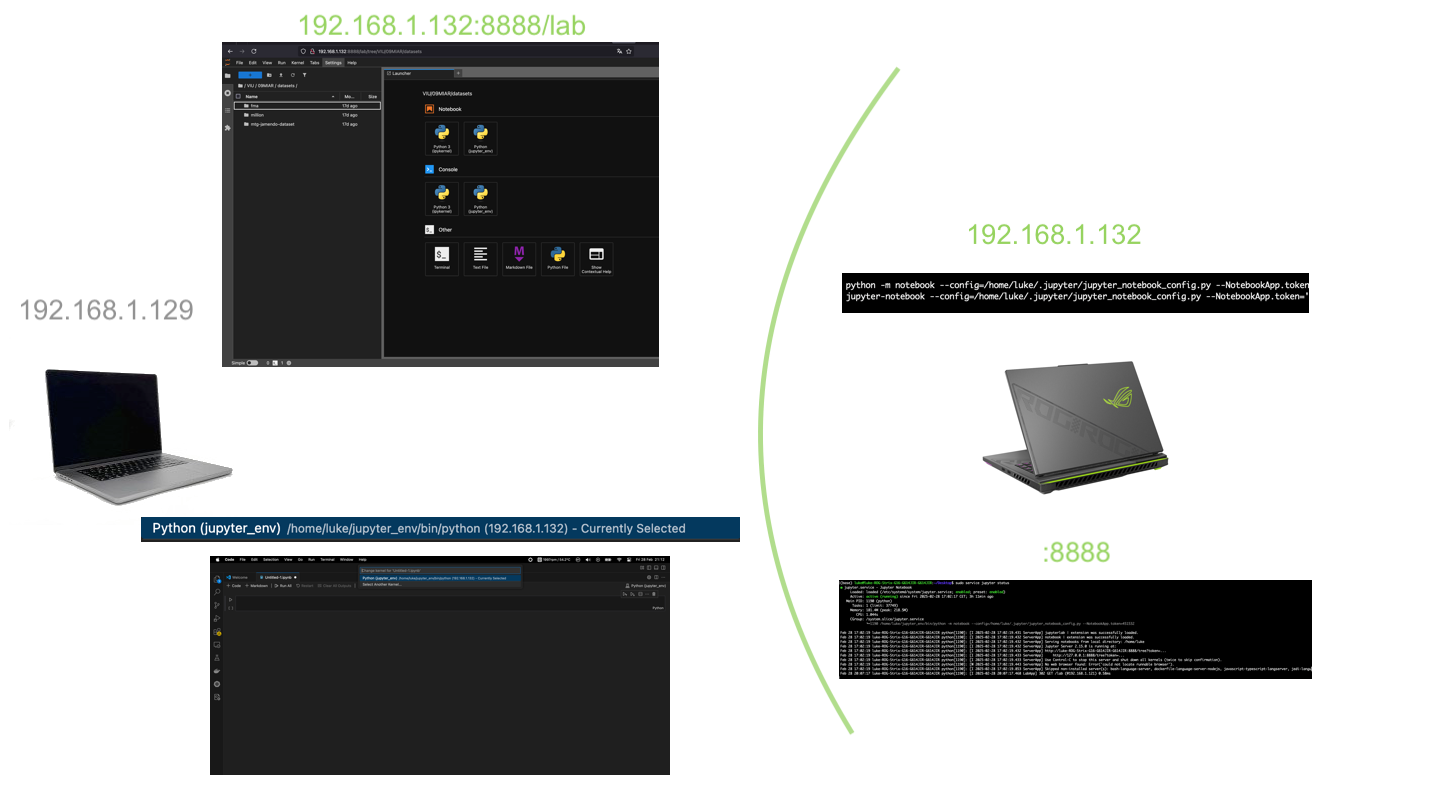
\includegraphics[width=0.9\textwidth]{images/jupyter-diagram.png}
\caption{Diagrama de conexión hardware.}
\label{fig:jupyter-diagram}
\end{figure}

Jupyter Lab estará esperando detrás del puerto 8888 de la máquina ASUS, la cual podrá ser instanciada por VistualStudio Code como Jupyter kernel o ser accesible vía explorador de Internet, pudiendo usar el entorno de edición y ejecución web que el servicio provee.

De esta manera se consigue usar toda la potencia de una máquina, desde la comodidad de uso y cercanía que brinda la otra.

\subsection{Modelos}



\section{Metodología}

Para el desarrollo de este TFM y del software que lo culminará, se han barajado 3 maneras, \emph{frameworks} o métodos de emprender y encaminar esta labor, de manera rigurosa, estructurada y ordenada. Los nombres que se han manejado han sido:
\begin{itemize}
    \item CRSIP-ML(Q): Cross Industry Standard Process for Machine Learning with Quality Assurance
    \item TDSP: Team Data Science Process
    \item Scrum: del rugby, ideal que significa trabajo en equipo y rápida respuesta de adaptación.
\end{itemize}

Cada una de estas tres herramientas aporta valor a cada uno de los pasos que se puedan llevar a cabo. Haciendo un análisis más profundo y tal y como se explica en la entrada web\cite{TDSP-PM}, se podría decir que \emph{TDSP} podría ser la combinación de \emph{Scrum} y \emph{CRISP-DM} (Cross Industry Standard Process for Data Mining. En el caso de proyectos de Machine Learning, CRISP-ML(Q) parte de la misma filosfía y se adapta a las necesidades específicas de este tipo de trabjos). Así pues, dado que todo lo referente a gestión de equipo y recursos en paralelo es innecesario, pues este trabajo se realiza por una sola persona, se ha decidido tomar un combinación de \textbf{CRISP-ML(Q)} y \textbf{Scrum}, que permita ser tan riguroso como el primero de ellos y tan ágil y potente en cuanto a herramientas, como el segundo.

\subsection{CRISP-ML(Q)}

\begin{figure}[H]
    \centering
    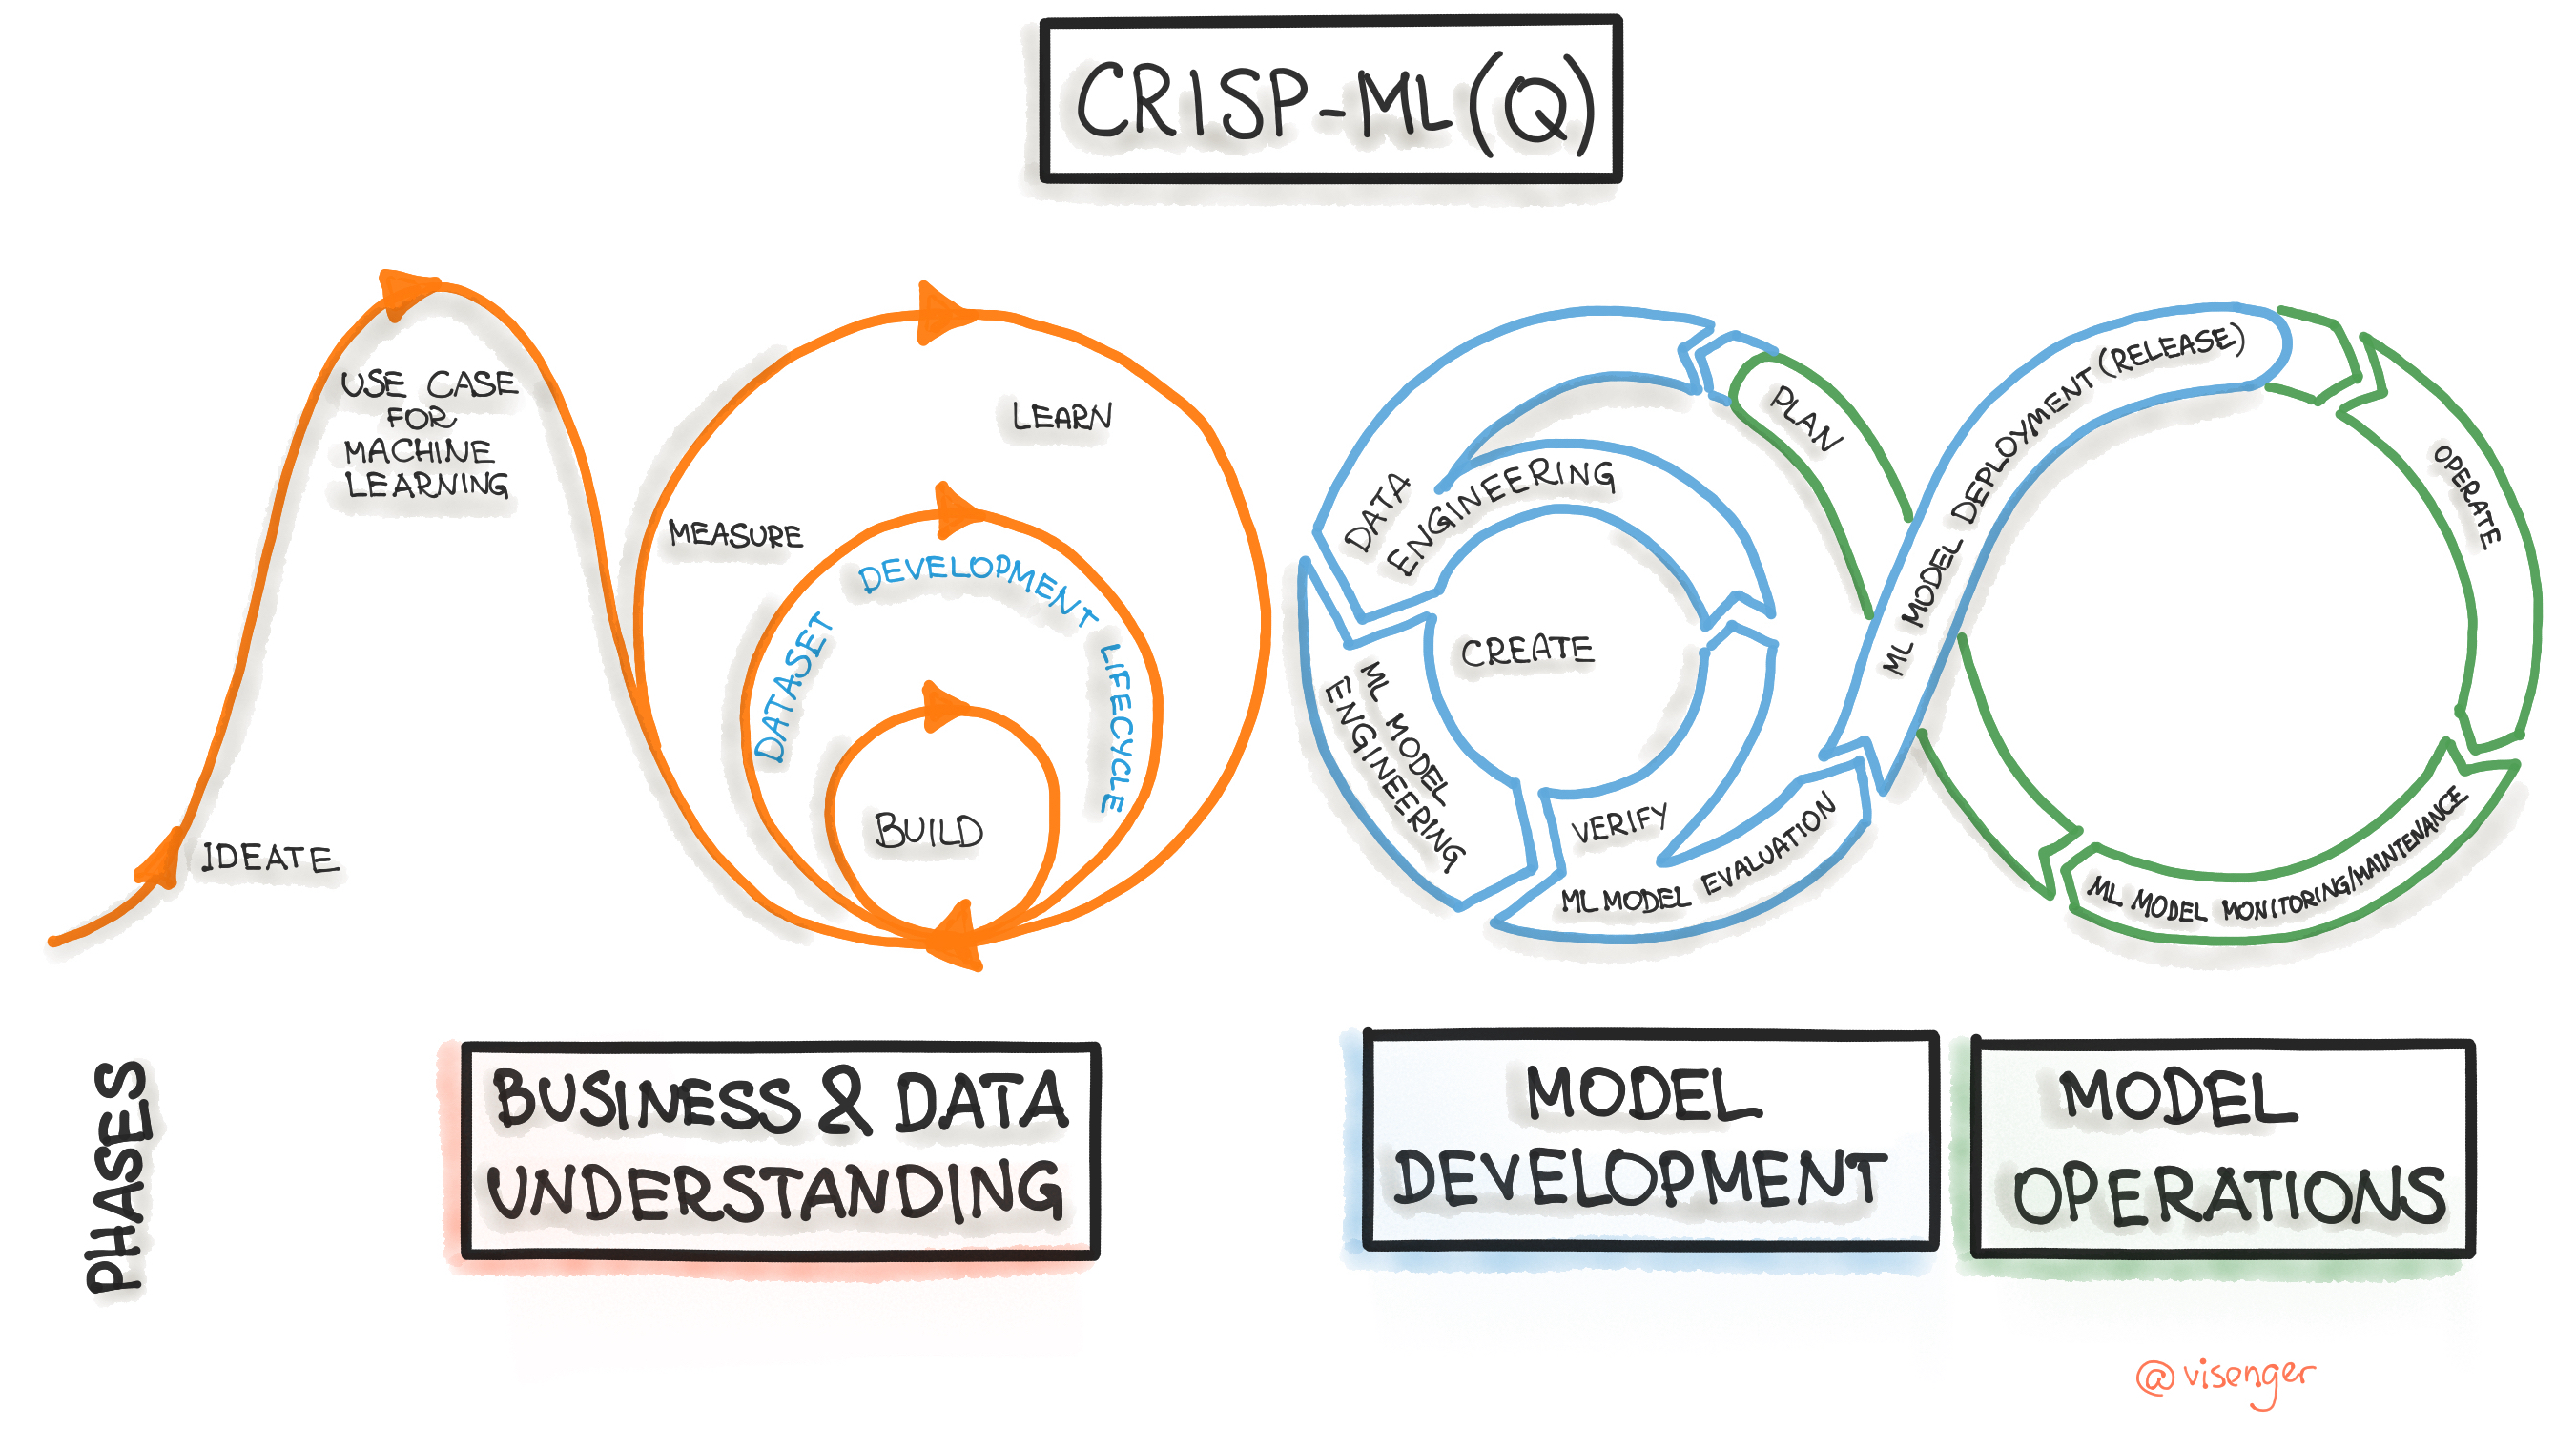
\includegraphics[width=0.9\textwidth]{images/crisp-ml-process.jpg}
    \caption{Diagrama de flujo usado en el desarrollo. Tomado de \cite{crispml}.}
    \label{fig:crispml-q-diagram}
  \end{figure}

\emph{CRISP-ML(Q)} conforma un marco estructurado para el desarrollo de proyectos de Machine Learning. Se compone de seis fases:

\begin{enumerate}
    \item \textbf{Comprensión del negocio}: Definir el problema y los objetivos del modelo.
    \item \textbf{Comprensión de los datos}: Recopilación y exploración inicial de los datos.
    \item \textbf{Preparación de los datos}: Limpieza, transformación y selección de variables.
    \item \textbf{Modelado}: Entrenamiento y optimización de modelos de Machine Learning.
    \item \textbf{Evaluación}: Validación de métricas y análisis del rendimiento.
    \item \textbf{Implementación y monitoreo}: Despliegue del modelo y seguimiento en producción.
\end{enumerate}

En la imagen\ref{fig:crispml-q-diagram} se puede ver cómo será el diagrama de flujo del desarrollo a seguir con este método.

\subsection{Scrum}

\emph{Scrum} es un framework que proporciona herramientas para la gestión ágil de proyectos de manera iterativa, dividiendo el trabajo en sprints (iteraciones cortas de 1-2 semanas). Las herramientas de \emph{Scrum} que se tomen para este proyecto serán:

\begin{itemize}
    \item \textbf{Product Backlog}: Lista priorizada de tareas a realizar.
    \item \textbf{Sprints}: Iteraciones donde se completan tareas específicas. Semanales.
    \item \textbf{Sprint Reviews}: Evaluaciones de cada sprint (semana o bisemanal) con la tutora de este TFM.
\end{itemize}

\subsection{Integración de CRISP-ML(Q) y Scrum}

A continuación, se detalla la planificación del TFM en base a estos marcos metodológicos.

\subsection{Product Backlog (Pila de producto)}

Las tareas que se han de llevar a cabo para completar el TFM, incluidos desarrollo de la documentación, software y evaluación y mantenimiento, se han organizado en el siguiente \emph{backlog}:

% \begin{table}[h]
%     \centering
    
%     \resizebox{\textwidth}{!}{
%     \begin{tabular}{|c|c|p{8cm}|c|}
%         \hline
%         \textbf{Épica} & \textbf{Historia de Usuario} & \textbf{Tareas} & \textbf{Prioridad} \\
%         \hline
%         Comprensión del negocio & Definir el problema & Redactar introducción, revisar 10 artículos, definir impacto y KPIs & Alta \\
%         \hline
%         Comprensión de los datos & Analizar calidad de los datos & Inspeccionar valores nulos, outliers, generar gráficos EDA & Alta \\
%         \hline
%         Preparación de los datos & Preprocesamiento de datos & Normalizar, codificar variables, dividir en train/test & Media \\
%         \hline
%         Modelado & Entrenar modelos de ML & Implementar baseline, probar algoritmos, ajustar hiperparámetros & Alta \\
%         \hline
%         Evaluación & Validar rendimiento del modelo & Comparar métricas, generar reportes de resultados & Alta \\
%         \hline
%         Implementación y monitoreo & Redactar el TFM & Documentar metodología, resultados, preparar presentación & Alta \\
%         \hline
%     \end{tabular}}
% \end{table}

\begin{table}[h]
    \centering
    \caption{Product Backlog (Pila de producto) del TFM basado en CRISP-ML(Q) y Scrum}
    \resizebox{0.8\textwidth}{!}{
    \begin{tabular}{|c|p{8cm}|p{8cm}|}
        \hline
        \textbf{Épica (Fase CRISP-ML(Q))} & \textbf{Historia de Usuario} & \textbf{Tareas} \\
        \hline
        Comprensión del negocio &  Como estudiante, quiero comprender bien el problema para entender el alcance del proyecto. & 
        \begin{itemize}
            \item Redactar introducción.
            \item Definir objetivos generales y específicos.
            \item Entender y tomar notas sobre el alcance del proyecto.
        \end{itemize} \\
        \hline
        Comprensión del negocio & Como estudiante, en mi labor de investigación, quiero revisar literatura existente en torno al problema.  &
        \begin{itemize}
            \item Buscar y analizar artículos y publicaciones relevantes. 
            \item Extraer ideas clave.
            \item Identificar tendencias en el estado del arte.
        \end{itemize} \\
        \hline
        Comprensión de los datos & Como estudiante, emulando a un científico de datos, quiero inspeccionar los datos disponibles para evaluar su calidad. & 
        \begin{itemize}
            \item Encontrar fuentes con datasets adecuados.
            \item Revisar estructura y tipos de datos.
            \item Evaluar insuficiencia, sesgo o desbalanceo en los datos.
            \item Escribir la metodología detallada.
        \end{itemize} \\
        \hline
        Preparación de los datos & Como estudiante y desarrollador, quiero limpiar y transformar los datos para que sean aptos para el modelo. & 
        \begin{itemize}
            \item Normalizar y codificar variables.
            \item Manejar valores atípicos y nulos.
        \end{itemize} \\
        \hline
        Preparación de los datos & Como estudiante y desarrollador, quiero dividir los datos en conjuntos de entrenamiento, validación y prueba. & 
        \begin{itemize}
            \item Definir proporción de separación de datos.
            \item Verificar balanceo de clases.
        \end{itemize} \\
        \hline
        Modelado & Como estudiante, emulando a un científico de datos, quiero entrenar un modelo base para establecer un punto de comparación. & 
        \begin{itemize}
            \item Entrenar el VAE.
            \item Evaluar rendimiento inicial.
            \item Extraer los primeros resultados.
        \end{itemize} \\
        \hline
        Modelado & Como estudiante, emulando a un científico de datos, quiero entrenar un modelo basado en GAN-Transformer y evaluar su precisión. & 
        \begin{itemize}
            \item Implementar y entrenar el modelo GAN-Transformer.
            \item Comparar modelos con métricas clave.
        \end{itemize} \\
        \hline
        Evaluación & Como estudiante e investigador, quiero evaluar el rendimiento del modelo para justificar su efectividad. &
        \begin{itemize}
            \item Calcular precisión, recall y F1-score.
            \item Generar matriz de confusión.
            \item Comparar modelos.
        \end{itemize} \\
        \hline
        Evaluación & Como estudiante e investigador, quiero establecer métricas comparativas entre los enfoques y mejorar la red GAN. & 
        \begin{itemize}
            \item Analizar interpretabilidad de los resultados.
            \item Ajustar hiperparámetros y arquitectura.
        \end{itemize} \\
        \hline
        Implementación y monitoreo & Como estudiante, quiero documentar la metodología utilizada para su presentación y evaluación. & 
        \begin{itemize}
            \item Documentar pruebas de los modelos.
            \item Preparar informe técnico.
        \end{itemize} \\
        \hline
        Implementación y monitoreo & Como estudiante, quiero preparar una presentación clara y concisa para la defensa del TFM. & 
        \begin{itemize}
            \item Diseñar diapositivas con gráficos y métricas.
            \item Exponer conclusiones.
            \item Practicar la presentación.
        \end{itemize} \\
        \hline
    \end{tabular}}
\end{table}


\clearpage
\begin{tcolorbox}[colback=black!85!white, colframe=orange!60!black, fontupper=\color{white},
    title=\textbf{\huge Product Backlog (Pila de producto)}, fonttitle=\color{white}]
    
        \begin{center}
        \renewcommand{\arraystretch}{0.2} % Reduce la separación entre filas
        \setlength{\tabcolsep}{8pt} % Reduce la separación entre columnas
        \resizebox{0.8\textwidth}{!}{ % Ajusta la tabla al 95% del ancho del texto
        \begin{tabular}{m{0.32\textwidth}<{\raggedright} m{0.32\textwidth}<{\raggedright} m{0.32\textwidth}<{\raggedright}} % 3 COLUMNAS BALANCEADAS
        
            %%%% FILA 1 - Comprensión del negocio (CN)
            \begin{tcolorbox}[colback=yellow!70!white, colframe=yellow!90!white, title={\textbf{CN-1}}, fonttitle=\color{black}]
            Redactar introducción.
            \end{tcolorbox} &        
            \begin{tcolorbox}[colback=yellow!70!white, colframe=yellow!90!white, title={\textbf{CN-2}}, fonttitle=\color{black}]
            Definir objetivos generales y específicos.
            \end{tcolorbox} &        
            \begin{tcolorbox}[colback=yellow!70!white, colframe=yellow!90!white, title={\textbf{CN-3}}, fonttitle=\color{black}]
            Entender y tomar notas sobre el alcance del proyecto.
            \end{tcolorbox} \\
    
            %%%% FILA 2
            \begin{tcolorbox}[colback=yellow!70!white, colframe=yellow!90!white, title={\textbf{CN-4}}, fonttitle=\color{black}]
            Buscar y analizar artículos y publicaciones relevantes.
            \end{tcolorbox} &
            \begin{tcolorbox}[colback=yellow!70!white, colframe=yellow!90!white, title={\textbf{CN-5}}, fonttitle=\color{black}]
            Extraer ideas clave.
            \end{tcolorbox} &
            \begin{tcolorbox}[colback=yellow!70!white, colframe=yellow!90!white, title={\textbf{CN-6}}, fonttitle=\color{black}]
            Identificar tendencias en el estado del arte.
            \end{tcolorbox} \\
    
            %%%% FILA 3 - Comprensión de los datos (CD)
            \begin{tcolorbox}[colback=purple!30!white, colframe=purple!40!white, title={\textbf{CD-1}}, fonttitle=\color{black}]
            Encontrar fuentes con datasets adecuados.
            \end{tcolorbox} &
            \begin{tcolorbox}[colback=purple!30!white, colframe=purple!40!white, title={\textbf{CD-2}}, fonttitle=\color{black}]
            Revisar estructura y tipos de datos.
            \end{tcolorbox} &
            \begin{tcolorbox}[colback=purple!30!white, colframe=purple!40!white, title={\textbf{CD-3}}, fonttitle=\color{black}]
            Evaluar insuficiencia, sesgo o desbalanceo en los datos.
            \end{tcolorbox} \\
    
            %%%% FILA 4
            \begin{tcolorbox}[colback=purple!30!white, colframe=purple!40!white, title={\textbf{CD-4}}, fonttitle=\color{black}]
            Escribir la metodología detallada.
            \end{tcolorbox} &
            \begin{tcolorbox}[colback=green!50!yellow, colframe=green!80!yellow, title={\textbf{PD-1}}, fonttitle=\color{black}]
            Normalizar y codificar variables.
            \end{tcolorbox} &
            \begin{tcolorbox}[colback=green!50!yellow, colframe=green!80!yellow, title={\textbf{PD-2}}, fonttitle=\color{black}]
            Manejar valores atípicos y nulos.
            \end{tcolorbox} \\
            \begin{tcolorbox}[colback=green!50!yellow, colframe=green!80!yellow, title={\textbf{PD-3}}, fonttitle=\color{black}]
            Definir proporción de separación de datos.
            \end{tcolorbox} &
    
            %%%% FILA 5
            \begin{tcolorbox}[colback=green!50!yellow, colframe=green!80!yellow, title={\textbf{PD-4}}, fonttitle=\color{black}]
            Verificar balanceo de clases.
            \end{tcolorbox} &
            \begin{tcolorbox}[colback=pink!60!red, colframe=pink!40!red, title={\textbf{M-1}}, fonttitle=\color{black}]
            Entrenar el VAE.
            \end{tcolorbox} \\
            \begin{tcolorbox}[colback=pink!60!red, colframe=pink!40!red, title={\textbf{M-2}}, fonttitle=\color{black}]
            Evaluar rendimiento inicial.
            \end{tcolorbox} &
    
            %%%% FILA 6
            \begin{tcolorbox}[colback=pink!60!red, colframe=pink!40!red, title={\textbf{M-3}}, fonttitle=\color{black}]
            Extraer los primeros resultados.
            \end{tcolorbox} &
            \begin{tcolorbox}[colback=pink!60!red, colframe=pink!40!red, title={\textbf{M-4}}, fonttitle=\color{black}]
            Implementar y entrenar el modelo GAN-Transformer.
            \end{tcolorbox} \\
            
            \begin{tcolorbox}[colback=pink!60!red, colframe=pink!40!red, title={\textbf{M-5}}, fonttitle=\color{black}]
            Comparar modelos con métricas clave.
            \end{tcolorbox} &
            \begin{tcolorbox}[colback=orange!70!white, colframe=orange!90!white, title={\textbf{EV-1}}, fonttitle=\color{black}]
            Calcular precisión, recall y F1-score.
            \end{tcolorbox} &
            \begin{tcolorbox}[colback=orange!70!white, colframe=orange!90!white, title={\textbf{EV-2}}, fonttitle=\color{black}]
            Generar matriz de confusión.
            \end{tcolorbox}
            \\

            %%%% FILA 8
            \begin{tcolorbox}[colback=orange!70!white, colframe=orange!90!white, title={\textbf{EV-3}}, fonttitle=\color{black}]
                Comparar modelos.
                
                \end{tcolorbox}
            &
            
            \begin{tcolorbox}[colback=orange!70!white, colframe=orange!90!white, title={\textbf{EV-4}}, fonttitle=\color{black}]
                Analizar interpretabilidad de los resultados.
                \end{tcolorbox} &

                \begin{tcolorbox}[colback=orange!70!white, colframe=orange!90!white, title={\textbf{EV-5}}, fonttitle=\color{black}]
                    Ajustar hiperparámetros y arquitectura.
                    \end{tcolorbox} 

            \\
    
            %%%% FILA 9
            
            \begin{tcolorbox}[colback=blue!30!white, colframe=blue!40!white, title={\textbf{IM-1}}, fonttitle=\color{black}]
            Documentar pruebas de los modelos.
            \end{tcolorbox} &
            \begin{tcolorbox}[colback=blue!30!white, colframe=blue!40!white, title={\textbf{IM-2}}, fonttitle=\color{black}]
            Preparar informe técnico.
            \end{tcolorbox} &
    
            %%%% FILA 10
            \begin{tcolorbox}[colback=blue!30!white, colframe=blue!40!white, title={\textbf{IM-3}}, fonttitle=\color{black}]
            Diseñar diapositivas con gráficos y métricas.
            \end{tcolorbox} \\
            \begin{tcolorbox}[colback=blue!30!white, colframe=blue!40!white, title={\textbf{IM-4}}, fonttitle=\color{black}]
            Exponer conclusiones.
            \end{tcolorbox} &
            \begin{tcolorbox}[colback=blue!30!white, colframe=blue!40!white, title={\textbf{IM-5}}, fonttitle=\color{black}]
            Practicar la presentación.
            \end{tcolorbox} \\
    
        \end{tabular}
        }
        \end{center}
    
    \end{tcolorbox}
    
\clearpage
% \begin{table}[h]
    \centering
    \caption{Estado ``actual'' de progreso del TFM basado en CRISP-ML(Q) y Scrum}
    \resizebox{\textwidth}{!}{
    \begin{tabular}{|p{8cm}|c|p{2.5cm}|}
        \hline
        \textbf{Tarea} & \textbf{Categoría\hfill \break CRISP-ML(Q) / (Código)} & \textbf{Estado} \\
        \hline
        Redactar introducción & Comprensión del negocio / (CN-1) & \ding{51}Hecho \\
        \hline
        Definir objetivos generales y específicos & Comprensión del negocio / (CN-2) & \ding{51}Hecho \\
        \hline
        Entender y tomar notas sobre el alcance del proyecto & Comprensión del negocio / (CN-3) & \ding{51}Hecho \\
        \hline
        Buscar y analizar artículos y publicaciones relevantes & Comprensión del negocio / (CN-4) & \ding{51}Hecho \\
        \hline
        Extraer ideas clave & Comprensión del negocio / (CN-5) & \ding{51}Hecho \\
        \hline
        Identificar tendencias en el estado del arte & Comprensión del negocio / (CN-6) & \ding{51}Hecho \\
        \hline
        Encontrar fuentes con datasets adecuados & Comprensión de los datos / (CD-1) & \ding{51}Hecho \\
        \hline
        Revisar estructura y tipos de datos & Comprensión de los datos / (CD-2) & \ding{51}Hecho \\
        \hline
        Evaluar insuficiencia, sesgo o desbalanceo en los datos & Comprensión de los datos / (CD-3) & \ding{45}En progreso \\
        \hline
        Escribir la metodología detallada & Implementación y monitoreo / (CD-4) & \ding{51}Hecho \\
        \hline
        Normalizar y codificar variables & Preparación de los datos / (PD-1) & \ding{43}Por hacer \\
        \hline
        Manejar valores atípicos y nulos & Preparación de los datos / (PD-2) & \ding{43}Por hacer \\
        \hline
        Definir proporción de separación de datos & Preparación de los datos / (PD-3) & \ding{43}Por hacer \\
        \hline
        Verificar balanceo de clases & Preparación de los datos / (PD-4) & \ding{43}Por hacer \\
        \hline
        Entrenar el VAE & Modelado / (M-1) & \ding{43}Por hacer \\
        \hline
        Evaluar rendimiento inicial & Modelado / (M-2) & \ding{43}Por hacer \\
        \hline
        Extraer los primeros resultados & Modelado / (M-3) & \ding{43}Por hacer \\
        \hline
        Implementar y entrenar el modelo GAN-Transformer & Modelado / (M-4) & \ding{43}Por hacer \\
        \hline
        Comparar modelos con métricas clave & Modelado / (M-5) & \ding{43}Por hacer \\
        \hline
        Analizar interpretabilidad de los resultados & Evaluación / (EV-1) & \ding{43}Por hacer \\
        \hline
        Calcular precisión, recall y F1-score & Evaluación / (EV-2) & \ding{43}Por hacer \\
        \hline
        Generar matriz de confusión & Evaluación / (EV-3) & \ding{43}Por hacer \\
        \hline
        Comparar modelos & Evaluación / (EV-4) & \ding{43}Por hacer \\
        \hline
        Ajustar hiperparámetros y arquitectura & Evaluación / (EV-5) & \ding{43}Por hacer \\
        \hline
        Documentar pruebas de los modelos & Implementación y monitoreo / (IM-1) & \ding{43}Por hacer \\
        \hline
        Preparar informe técnico & Implementación y monitoreo / (IM-2) & \ding{43}Por hacer \\
        \hline
        Diseñar diapositivas con gráficos y métricas & Implementación y monitoreo / (IM-3) & \ding{43}Por hacer \\
        \hline
        Exponer conclusiones & Implementación y monitoreo / (IM-4) & \ding{43}Por hacer \\
        \hline
        Practicar la presentación & Implementación y monitoreo / (IM-5) & \ding{43}Por hacer \\
        \hline
    \end{tabular}}
\end{table}

Estableciendo las ``rondas'' iterables de progreso en \emph{sprints} de Scrum, el siguiente \emph{kanban} ilustra el estado ``actual'' del progreso de este trabajo:
\begin{tcolorbox}[colback=black!85!white, colframe=orange!60!black, fontupper=\color{white},
    title=\textbf{\huge Kanban}, fonttitle=\color{white}]
    {\huge \emph{Sprint 3}}
        \begin{center}
            \renewcommand{\arraystretch}{0.2} % Reduce la separación entre filas
            \setlength{\tabcolsep}{8pt} % Reduce la separación entre columnas
            \resizebox{\textwidth}{!}{ % Ajusta la tabla al 95% del ancho del texto
            \begin{tabular}{m{4cm} m{4cm} m{4cm} m{4cm} m{4cm}}
            \begin{center}
            {\Fontauri \huge \emph{to do}}
            \end{center}
            & \begin{center}
            {\Fontauri \huge \emph{to do}} 
            \end{center}
            & \begin{center}
            {\Fontauri \huge \emph{to do}} 
            \end{center}
            & \begin{center}
            {\Fontauri \huge \emph{in progress}} 
            \end{center} 
            & \begin{center}
            {\Fontauri \huge \emph{done}} 
            \end{center} \\
            
            \begin{tcolorbox}[colback=green!50!white, colframe=green!80!black, title={\textbf{PD-1}}, fonttitle=\color{black}]
            Normalizar y codificar variables.
            \end{tcolorbox} &
            \begin{tcolorbox}[colback=green!50!white, colframe=green!80!black, title={\textbf{PD-2}}, fonttitle=\color{black}]
            Manejar valores atípicos y nulos.
            \end{tcolorbox} &
            \begin{tcolorbox}[colback=green!50!white, colframe=green!80!black, title={\textbf{PD-3}}, fonttitle=\color{black}]
            Definir proporción de separación de datos.
            \end{tcolorbox} &
            \begin{tcolorbox}[colback=purple!30!white, colframe=purple!40!white, title={\textbf{CD-3}}, fonttitle=\color{black}]
            Evaluar insuficiencia, sesgo o desbalanceo en los datos.
            \end{tcolorbox} &
            \begin{tcolorbox}[colback=yellow!70!white, colframe=yellow!90!white, title={\textbf{CN-1}}, fonttitle=\color{black}]
            Redactar introducción.
            \end{tcolorbox}
            \\

            \begin{tcolorbox}[colback=green!50!white, colframe=green!80!black, title={\textbf{PD-4}}, fonttitle=\color{black}]
            Verificar balanceo de clases.
            \end{tcolorbox} &
            \begin{tcolorbox}[colback=pink!60!red, colframe=pink!40!red, title={\textbf{M-1}}, fonttitle=\color{black}]
            Entrenar el VAE.
            \end{tcolorbox} &
            \begin{tcolorbox}[colback=pink!60!red, colframe=pink!40!red, title={\textbf{M-2}}, fonttitle=\color{black}]
            Evaluar rendimiento inicial.
            \end{tcolorbox} &
            &
            \begin{tcolorbox}[colback=yellow!70!white, colframe=yellow!90!white, title={\textbf{CN-2}}, fonttitle=\color{black}]
            Definir objetivos generales y específicos.
            \end{tcolorbox}
            \\
            
            \begin{tcolorbox}[colback=pink!60!red, colframe=pink!40!red, title={\textbf{M-3}}, fonttitle=\color{black}]
            Extraer los primeros resultados.
            \end{tcolorbox} & 
            \begin{tcolorbox}[colback=pink!60!red, colframe=pink!40!red, title={\textbf{M-4}}, fonttitle=\color{black}]
            Implementar y entrenar el modelo GAN-Transformer.
            \end{tcolorbox} &
            \begin{tcolorbox}[colback=pink!60!red, colframe=pink!40!red, title={\textbf{M-5}}, fonttitle=\color{black}]
            Comparar modelos con métricas clave.
            \end{tcolorbox} &
            & 
            \begin{tcolorbox}[colback=yellow!70!white, colframe=yellow!90!white, title={\textbf{CN-3}}, fonttitle=\color{black}]
            Entender y tomar notas sobre el alcance del proyecto.
            \end{tcolorbox} 
            \\

            \begin{tcolorbox}[colback=orange!70!white, colframe=orange!90!white, title={\textbf{EV-1}}, fonttitle=\color{black}]
            Analizar interpretabilidad de los resultados.
            \end{tcolorbox} & 
            \begin{tcolorbox}[colback=orange!70!white, colframe=orange!90!white, title={\textbf{EV-2}}, fonttitle=\color{black}]
            Calcular precisión, recall y F1-score.
            \end{tcolorbox} &
            \begin{tcolorbox}[colback=orange!70!white, colframe=orange!90!white, title={\textbf{EV-3}}, fonttitle=\color{black}]
            Generar matriz de confusión.
            \end{tcolorbox} &
            &
            \begin{tcolorbox}[colback=yellow!70!white, colframe=yellow!90!white, title={\textbf{CN-4}}, fonttitle=\color{black}]
            Buscar y analizar artículos y publicaciones relevantes.
            \end{tcolorbox}    
            \\
    
            
            \begin{tcolorbox}[colback=orange!70!white, colframe=orange!90!white, title={\textbf{EV-4}}, fonttitle=\color{black}]
            Comparar modelos.
            \end{tcolorbox} &
            \begin{tcolorbox}[colback=orange!70!white, colframe=orange!90!white, title={\textbf{EV-5}}, fonttitle=\color{black}]
            Ajustar hiperparámetros y arquitectura.
            \end{tcolorbox} &
            \begin{tcolorbox}[colback=blue!30!white, colframe=blue!40!white, title={\textbf{IM-1}}, fonttitle=\color{black}]
            Documentar pruebas de los modelos.
            \end{tcolorbox} &
            &
            \begin{tcolorbox}[colback=yellow!70!white, colframe=yellow!90!white, title={\textbf{CN-5}}, fonttitle=\color{black}]
            Extraer ideas clave.
            \end{tcolorbox} 
            \\
            
            \begin{tcolorbox}[colback=blue!30!white, colframe=blue!40!white, title={\textbf{IM-2}}, fonttitle=\color{black}]
            Preparar informe técnico.
            \end{tcolorbox} &
            \begin{tcolorbox}[colback=blue!30!white, colframe=blue!40!white, title={\textbf{IM-3}}, fonttitle=\color{black}]
            Diseñar diapositivas con gráficos y métricas.
            \end{tcolorbox} &
            \begin{tcolorbox}[colback=blue!30!white, colframe=blue!40!white, title={\textbf{IM-4}}, fonttitle=\color{black}]
            Exponer conclusiones.
            \end{tcolorbox} &
            &
            \begin{tcolorbox}[colback=yellow!70!white, colframe=yellow!90!white, title={\textbf{CN-6}}, fonttitle=\color{black}]
            Identificar tendencias en el estado del arte.
            \end{tcolorbox} 
            \\
    
            \begin{tcolorbox}[colback=blue!30!white, colframe=blue!40!white, title={\textbf{IM-5}}, fonttitle=\color{black}]
            Practicar la presentación.
            \end{tcolorbox} &
            &&&
            \begin{tcolorbox}[colback=purple!30!white, colframe=purple!40!white, title={\textbf{CD-1}}, fonttitle=\color{black}]
            Encontrar fuentes con datasets adecuados.
            \end{tcolorbox}
            \\
    
            
            &&&&
            \begin{tcolorbox}[colback=purple!30!white, colframe=purple!40!white, title={\textbf{CD-2}}, fonttitle=\color{black}]
            Revisar estructura y tipos de datos.
            \end{tcolorbox} 
            \\

            &&&&
            \begin{tcolorbox}[colback=purple!30!white, colframe=purple!40!white, title={\textbf{CD-4}}, fonttitle=\color{black}]
            Escribir la metodología detallada.
            \end{tcolorbox} 
            \\
        \end{tabular}}
        \end{center}
    
    \end{tcolorbox}
    
%\begin{tcolorbox}[colback=black!85!white, colframe=orange!60!black, fontupper=\color{white},
title=\textbf{\huge Kanban}, fonttitle=\color{white}]

{\huge \emph{Sprint 3}}
    \begin{center}
    \resizebox{0.8\textwidth}{!}{\begin{tabular}{m{4cm} m{4cm} m{4cm}}
        \begin{center}
        {\Fontauri \huge \emph{to do}}
        \end{center}
        & \begin{center}
        {\Fontauri \huge \emph{in progress}} 
        \end{center} & 
        \begin{center}{\Fontauri \huge \emph{done}} 
        \end{center} \\
        
        \begin{tcolorbox}[colback=green!50!white, colframe=green!80!black,
            title={\textbf{PD-2}}, 
            fonttitle=\color{black}
        ]
        Normalización y codificación de variables.
        \end{tcolorbox} & \begin{tcolorbox}[colback=purple!30!white, colframe=purple!40!white,
            title={\textbf{CD-3}}, 
            fonttitle=\color{black}
        ]
        Identificar valores nulos y outliers.
        \end{tcolorbox} 
        &
        \resizebox{0.8\textwidth}{!}{\begin{tabular}{m{4cm} m{4cm} m{4cm}}
        \begin{tcolorbox}[colback=yellow!70!white, colframe=yellow!90!white,
            title={\textbf{CN-1}}, 
            fonttitle=\color{black}
        ]
        \vspace{0.3cm}
        Definir problema del TFM.
        \end{tcolorbox}
        & 
        \begin{tcolorbox}[colback=yellow!70!white, colframe=yellow!90!white,
            title={\textbf{CN-2}}, 
            fonttitle=\color{black}
        ]
        Revisar al menos 10 artículos.
        \end{tcolorbox} 
        & 
        \begin{tcolorbox}[colback=yellow!70!white, colframe=yellow!90!white,
            title={\textbf{CN-3}}, 
            fonttitle=\color{black}
        ]
        Definir métricas clave (KPIs).
        \end{tcolorbox} 
        \\
        \end{tabular}
        }
        

        \\
        \begin{tcolorbox}[colback=green!50!white, colframe=green!80!black,
            title={\textbf{PD-3}}, 
            fonttitle=\color{black}
        ]
        Dividir dataset en train/val/test.
        \end{tcolorbox} & \begin{tcolorbox}[colback=green!50!white, colframe=green!80!black,
            title={\textbf{PD-1}}, 
            fonttitle=\color{black}
        ]
        Limpieza y preprocesamiento de datos.
        \end{tcolorbox} &
        
        \\
        \begin{tcolorbox}[colback=pink!60!red, colframe=pink!40!red,
            title={\textbf{M-1}}, 
            fonttitle=\color{black}
        ]
        Implementar modelo base (benchmark).
        \end{tcolorbox} & &
        
        \\
        
        \begin{tcolorbox}[colback=pink!60!red, colframe=pink!40!red,
            title={\textbf{M-2}}, 
            fonttitle=\color{black}
        ]
        Probar al menos 2-3 modelos.
        \end{tcolorbox} & &
        \begin{tcolorbox}[colback=purple!30!white, colframe=purple!40!white,
            title={\textbf{CD-1}}, 
            fonttitle=\color{black}
        ]
        \vspace{0.3cm}
        Recopilar datasets disponibles.
        \end{tcolorbox} 
        \\
        \begin{tcolorbox}[colback=pink!60!red, colframe=pink!40!red,
            title={\textbf{M-3}}, 
            fonttitle=\color{black}
        ]
        Ajustar hiperparámetros con GridSearch/Optuna.
        \end{tcolorbox} & &
        \begin{tcolorbox}[colback=purple!30!white, colframe=purple!40!white,
            title={\textbf{CD-2}}, 
            fonttitle=\color{black}
        ]
        Realizar análisis exploratorio (EDA).
        \end{tcolorbox} 
        \\
        \begin{tcolorbox}[colback=orange!70!white, colframe=orange!90!white,
            title={\textbf{Ev-1}}, 
            fonttitle=\color{black}
        ]
        Comparar métricas de rendimiento.
        \end{tcolorbox} & &
        \begin{tcolorbox}[colback=purple!30!white, colframe=purple!40!white,
            title={\textbf{CD-4}}, 
            fonttitle=\color{black}
        ]
        Generar visualización de datos.
        \end{tcolorbox}
        \\        
        \begin{tcolorbox}[colback=orange!70!white, colframe=orange!90!white,
            title={\textbf{Ev-2}}, 
            fonttitle=\color{black}
        ]
        Generar matriz de confusión.
        \end{tcolorbox}  &
        
        &
        \\
        \begin{tcolorbox}[colback=blue!30!white, colframe=blue!40!white,
            title={\textbf{IM-1}}, 
            fonttitle=\color{black}
        ]
        Preparar presentación final.
        \end{tcolorbox} & & \\
    
    \end{tabular}}
    \end{center}

\end{tcolorbox}
\clearpage
Como se puede apreciar, al haber un sólo desarrollador para el proyecto, no se han establecido y etiquetado asignaciones de tareas a recursos.

Además, dado el predominante carácter didáctico y explorativo del trabajo, no se ha querido (ni podido, pues una sola persona no debería estimar esfuerzos de tareas) llevar a cabo una estimación de coste o esfuerzo en cada una de las tareas.

Esto podría dar lugar a sprints desbalanceados, pero siendo francos y dada la necesidad imporiosa de conciliación familiar, laboral y estudiantil, marcar sprints rígidos a cumplir sería una toda osadía.

\subsection{Planificación del TFM}

Llegado a este punto, se ha hecho un ejercicio de recabado y asunción perpleja del método y pasos que hasta ahora se han ido siguiendo. Visto con perspectiva, desde el inicio de esta memoria se ha trabajado siguiendo los pasos detallados en \emph{CRISP-ML(Q)} y que se verán a continuación:

\begin{table}[h]
    \centering
    \resizebox{\textwidth}{!}{
    \begin{tabular}{|c|c|c|}
        \hline
        \textbf{Fase CRISP-ML(Q)} & \textbf{Sprints (Iteraciones)} & \textbf{Tareas principales} \\
        \hline
        Comprensión del negocio / (CN)& Sprint 1-2 
        \begin{tcolorbox}[colback=yellow!70!white, colframe=yellow!90!white,
        width=0.4cm,height=0.4cm]
        \end{tcolorbox} & Definir problema, revisar literatura, establecer métricas de éxito \\
        \hline
        Comprensión de los datos / (CD)& Sprint 3-4 
        \begin{tcolorbox}[colback=purple!30!white, colframe=purple!40!white,
        width=0.4cm,height=0.4cm]
        \end{tcolorbox} & Recopilación de datos, EDA, visualización de datos \\
        \hline
        Preparación de los datos / (PD) & Sprint 5-6
        \begin{tcolorbox}[colback=green!50!white, colframe=green!80!black,
        width=0.4cm,height=0.4cm]
        \end{tcolorbox} & Limpieza, normalización, codificación de variables \\
        \hline
        Modelado / (M) & Sprint 7-8 
        \begin{tcolorbox}[colback=pink!60!red, colframe=pink!40!red,
        width=0.4cm,height=0.4cm]
        \end{tcolorbox} & Implementación y ajuste de modelos de ML \\
        \hline
        Evaluación / (Ev) & Sprint 9-10 
        \begin{tcolorbox}[colback=orange!70!white, colframe=orange!90!white,
        width=0.4cm,height=0.4cm]
        \end{tcolorbox} & Comparación de métricas y validación del modelo \\
        \hline
        Implementación y monitoreo (IM) & Sprint 11-12
        \begin{tcolorbox}[colback=blue!30!white, colframe=blue!40!white,
        width=0.4cm,height=0.4cm]
        \end{tcolorbox} & Redacción de conclusiones, revisión y entrega \\
        \hline
    \end{tabular}}
    \caption{Planificación del TFM basado en CRISP-ML(Q) y Scrum}
\end{table}

Cada una de estas fases se ha dividido en \emph{sprints} de \emph{Scrum}, señalizados por un color distinto en el \emph{kanban}, lo que permite ver de manera directa el estado de cada \emph{sprint}.

Expuestas las fases de la planificación, se procede con el plan.

\subsubsection{Comprensión del negocio}

El objetivo del TFM es desarrollar un modelo basado en redes generativas adversariales (GANs) capaz de generar música personalizada en formato MP3. Se pretende que el modelo genere piezas musicales dentro de géneros específicos, con coherencia armónica y estructural.

Para ello, se han identificado los siguientes desafíos clave:
\begin{itemize}
    \item Disponibilidad y estructuración de datasets de música en formato MP3.
    \item Extracción y representación de características musicales relevantes bajo espectrogramas.
    \item Generar un modelo basado en Inteligencia Artificial que sea capaz de asociar características de la música, recogidas en los espectrogramas y asociarlas a un género aportado con cada ejemplo.
    \item Que ese mismo modelo de ``inteligente'' sea capaz de generar música aportando solamente el género requerido.
    \item Evaluación de la calidad de las composiciones generadas mediante métricas objetivas y subjetivas.
    \item Implementación de una interfaz para la generación de música personalizada.
\end{itemize}

Se justifica este trabajo en función del auge de los modelos generativos en el ámbito musical y la creciente demanda de herramientas que permitan la generación de contenido musical adaptado a los gustos del usuario.

\subsubsection{Comprensión de los datos}

El dataset utilizado para entrenar el modelo se compone de archivos MP3 extraídos de bases de datos como \textit{Free Music Archive} y \textit{MTG-Jamendo}. Estas fuentes proporcionan pistas en diferentes géneros, etiquetadas con metadatos detallados.

Se lleva a cabo un análisis exploratorio para comprender la estructura de los datos, incluyendo:
\begin{itemize}
    \item Distribución de duraciones y características tonales.
    \item Análisis espectral de los archivos de audio mediante espectrogramas y MFCCs.
    \item Identificación de posibles sesgos en la distribución de géneros y calidad del audio.
\end{itemize}

Se detecta la necesidad de normalización y preprocesamiento de los archivos para garantizar la calidad del entrenamiento del modelo.

\subsubsection{Preparación de los datos}

Se implementa un pipeline de procesamiento de audio que incluye las siguientes etapas:
\begin{itemize}
    \item Conversión de los archivos MP3 en espectrogramas.
    \item Normalización de amplitudes y ajuste de la frecuencia de muestreo para uniformizar los datos.
    \item Se probarán ventanas de \emph{sample} de audios de entre 10 - 25 y 40 milisegundos (se atenderá al criterio de calidad de generación obtenida y al consumo de recursos, capacidad y estabilidad del hardware disponible).
\end{itemize}

Estos pasos aseguran que el modelo aprenda patrones relevantes sin sesgos introducidos por diferencias en la calidad de grabación o características técnicas de los archivos de audio.

\subsubsection{Modelado}

El modelo propuesto se basa en una arquitectura de redes generativas adversariales (GANs) adaptadas a la generación de secuencias de audio en formato MP3. Se diseñan los siguientes componentes:
\begin{itemize}
    \item \textbf{Generador:} Recibe una entrada aleatoria y genera espectrogramas sintéticos, que luego son convertidos en archivos de audio mediante un vocoder neuronal.
    \item \textbf{Discriminador:} Evalúa la autenticidad de los espectrogramas generados, comparándolos con fragmentos reales del dataset.
\end{itemize}

Se experimenta con distintas configuraciones, incluyendo GANs convencionales y variantes como Wasserstein-GAN (WGAN) para mejorar la estabilidad del entrenamiento. También se incorpora un Transformer en la arquitectura del generador para reforzar la coherencia temporal de las secuencias generadas.

\subsubsection{Evaluación}

La evaluación del modelo se realiza desde dos enfoques complementarios:
\begin{itemize}
    \item \textbf{Métricas objetivas:} Se analizan características acústicas como la similitud espectral entre las composiciones generadas y las piezas originales del dataset.
    \item \textbf{Métricas subjetivas:} Se realiza una prueba con oyentes humanos para evaluar la percepción de calidad y coherencia de las piezas generadas.
\end{itemize}

Se establecen comparaciones con modelos previos como \textit{MusicVAE} y \textit{MuseGAN} para contextualizar los resultados obtenidos.

\subsubsection{Implementación y monitoreo}

El modelo final se despliega en una interfaz interactiva donde los usuarios pueden generar música personalizada ajustando parámetros como:
\begin{itemize}
    \item Género musical deseado.
    \item Complejidad rítmica y armónica.
    \item Instrumentación preferida.
\end{itemize}

Se establece un sistema de monitoreo que recopila datos sobre el uso del modelo y permite la mejora continua mediante aprendizaje activo. Se documenta todo el proceso para garantizar la reproducibilidad y facilitar futuras mejoras en la arquitectura del modelo.

\section{UML}

\subsection{Análisis del sistema}
\label{analisis-del-sistema}

Se ha elegido UML como método de diseño del software fruto de este Trabajo de Fin de Máster.

UML es un lenguaje de modelado de software que tiene sus propios mecanismos para llevar a cabo las tareas, desde la definición de lo
que serán los ``requisitos funcionales'': lo que se pretende que sea capaz de proporcionar el programa al usuario; hasta la definición de las clases que intervendrán en la codificación de la aplicación, así como cada flujo de información contemplado en el programa final.

\subsubsection{Formalización de la especificación de requisitos}

Los requisitos funcionales representan un manifiesto de todos los servicios que el programa proporcionará al usuario y cómo se comporta el sistema en cada una de las acciones llevadas a cabo para rendir esos servicios.

Los requisitos funcionales están denotados por la letra F, seguida de un guión y un número de requisito que lo clasificará como único en el sistema. Los requisitos funcionales de la aplicación son los siguientes:

\begin{itemize}

    \item F-1: el sistema debería dar la oportunidad al usuario de descargar una pieza musical según un género concreto:
    \begin{itemize}
        \item F-1.1: el sistema debería mostrar una lista de géneros musicales y dar la oportunidad al usuario de seleccionar uno de ellos.
        \item F-1.2: el sistema debería dar la oportunidad al usuario de instar la generación de una pieza musical que concuerde con el género seleccionado.
        \item F-1.3: el sistema debería dar la oportunidad de descargar la pieza musical generada
    \end{itemize}
    
    \item F-2: el sistema debería proporcionar la oportunidad de evaluar la pieza musical generada.
    \begin{itemize}
        \item F-2.1: el sistema debería proporcionar una manera de almacenar datos de cada evaluación.
    \end{itemize}
       
    \item F-3: el sistema debería dar la oportunidad al usuario de consultar una ayuda sobre el uso y comportamiento del programa.

\end{itemize}

\subsubsection{Diagramas de Casos de Uso del Sistema}

El siguiente paso a seguir en el proceso definido por UML es el diseño de casos de uso.

Los casos de uso representan todas las acciones que pueden realizar uno o más usuarios en cada momento con la aplicación que se modela. A continuación se definen cuáles son los diagramas de casos de uso del sistema.

Los casos de uso que se van describir son los siguientes:


\begin{itemize}

    \item PresentaciónDelSistema. Diagrama 1.

    \item GenerarPiezaMusical. Diagrama 2

    \item EvaluarPiezaMusicalGenerada. Diagrama 3.

\end{itemize}

\begin{enumerate}

\item{\textbf{Diagrama de Casos de Uso: PresentaciónDelSistema}}

\begin{figure}[H]
  \centering
  \includesvg[width=0.55\textwidth]{images/caso-uso-presentaciondelsistema.svg}
  \caption{Diagrama de caso de uso principal del sistema.}
  \label{fig:caso-uso-presentaciondelsistema}
\end{figure}

\begin{longtable}{|>{\columncolor[rgb]{0.75,0.75,0.75}}p{3cm}|p{11cm}|}
\caption{Caso de uso \emph{PresentaciónDelSistema.}} \\
\hline \centerline{\textcolor[rgb]{1.00,1.00,1.00}{\textbf{\small Nombre}}} & {\small PresentaciónDelSistema.}
\\
\hline \centerline{\textcolor[rgb]{1.00,1.00,1.00}{\textbf{\small
Descripción}}} & {\small Establecimiento de las relaciones entre los elementos internos del sistema y la interacción con los elementos externos, describiéndose la presentación principal del mismo.}
\\
\hline
\centerline{\textcolor[rgb]{1.00,1.00,1.00}{\textbf{\small
Actores}}}
&
{\small Usuario.}
\\
\hline
\begin{center}
\textcolor[rgb]{1.00,1.00,1.00}{\textbf{\small Casos de uso}}
\end{center}
\begin{center}

\end{center}
&

{\small \emph{GenerarPiezaMusical:} Permite al usuario solicitar la generación de una pieza musical.}

{\small \emph{ConsultarAyuda:} Permite al usuario consultar la ayuda
sobre el funcionamiento del programa.}
\\
\hline
\begin{center}
\end{center}
\begin{center}
\textcolor[rgb]{1.00,1.00,1.00}{\textbf{\small Flujo de eventos
principal}}
\end{center}
&
{\small Pasos de ejecución del camino básico del caso de uso:}

{\small
\begin{enumerate}
    \item El usuario accede al sistema.

    \item El sistema muestra las opciones que se pueden llevar a cabo.

    \item El usuario elige una de las opciones.
\end{enumerate}
}
\\
\hline \centerline{\textcolor[rgb]{1.00,1.00,1.00}{\textbf{\small
Flujo de eventos}}}
\centerline{\textcolor[rgb]{1.00,1.00,1.00}{\textbf{\small
excepcional}}} & {\small No se contempla.}
\\
\hline
\end{longtable}

\item{\textbf{Diagrama de Casos de Uso: GenerarPiezaMusical}}

\begin{figure}[H]
  \centering
  \includesvg[width=0.6\textwidth]{images/caso-uso-generarpiezamusical.svg}
  \caption{Diagrama de caso de uso de generación de una pieza musical.}
  \label{fig:caso-uso-generarpiezamusical}
\end{figure}

\begin{longtable}{|>{\columncolor[rgb]{0.75,0.75,0.75}}p{3cm}|p{11cm}|}
\caption{Caso de uso \emph{GenerarPiezaMusical.}} \\
\hline \centerline{\textcolor[rgb]{1.00,1.00,1.00}{\textbf{\small Nombre}}} & {\small GenerarPiezaMusical.}
\\
\hline \centerline{\textcolor[rgb]{1.00,1.00,1.00}{\textbf{\small Descripción}}} & {\small Representación de todas las acciones necesarias para generar una pieza musical.}
\\
\hline \centerline{\textcolor[rgb]{1.00,1.00,1.00}{\textbf{\small Actores}}} & {\small Usuario.}
\\
\hline
\begin{center}
\textcolor[rgb]{1.00,1.00,1.00}{\textbf{\small Casos de uso}}
\end{center}
\begin{center}

\end{center}
& {\small \emph{SolicitarPiezaMusical:} permite al usuario solicitar la generación de una
pieza musical.}

{\small \emph{SeleccionarGénero:} brinda al usuario la posibilidad de seleccionar el género de la pieza musical a generar.}

\\
\hline
\begin{center}
\end{center}
\begin{center}
\textcolor[rgb]{1.00,1.00,1.00}{\textbf{\small Flujo de eventos
principal}}
\end{center}
& {\small Pasos de ejecución del camino básico del caso de uso:}

{\small
\begin{enumerate}
    \item El usuario accede al sistema.

    \begin{enumerate}
        \item[] 1.1 El usuario selecciona un género musical de una lista dada.
        \item[] 1.2 El usuario solicita una muestra de música generada, asociada al género musical seleccionado.
        \item[] 1.3 El sistema devuelve la pieza musical generada.
    \end{enumerate}
\end{enumerate}
}
\\
\hline \centerline{\textcolor[rgb]{1.00,1.00,1.00}{\textbf{\small Flujo de eventos}}}
\centerline{\textcolor[rgb]{1.00,1.00,1.00}{\textbf{\small excepcional}}} & {\small No se contempla.}
\\
\hline
\end{longtable}

\item{\textbf{Diagrama de Casos de Uso: EvaluarPiezaMusicalGenerada}}

\begin{figure}[H]
  \centering
  \includesvg[width=0.58\textwidth]{images/caso-uso-evaluarpiezamusicalgenerada.svg}
  \caption{Diagrama de caso de uso de evaluación de una pieza musical.}
  \label{fig:caso-uso-evaluarpiezamusicalgenerada}
\end{figure}

\begin{longtable}{|>{\columncolor[rgb]{0.75,0.75,0.75}}p{3cm}|p{11cm}|}
\caption{Caso de uso \emph{EvaluarPiezaMusicalGenerada.}} \\
\hline \centerline{\textcolor[rgb]{1.00,1.00,1.00}{\textbf{\small
Nombre}}} & {\small EvaluarPiezaMusicalGenerada.}
\\
\hline \centerline{\textcolor[rgb]{1.00,1.00,1.00}{\textbf{\small
Descripción}}} & {\small Representación de las acciones necesarias para evaluar la pieza musical generada.}
\\
\hline \centerline{\textcolor[rgb]{1.00,1.00,1.00}{\textbf{\small
Actores}}} & {\small Usuario.}
\\
\hline
\begin{center}
\textcolor[rgb]{1.00,1.00,1.00}{\textbf{\small Casos de uso}}
\end{center}
\begin{center}

\end{center}
& {\small \emph{PuntuarPiezaMusical:} permite al usuario puntuar la pieza musical generada en base a su percepción subjetiva de pertenencia al género solicitado.}

{\small \emph{GenerarPiezaMusical:} permite al usuario solicitar la genearción de una pieza musical, dado un género concreto y descargarla.}

\\
\hline
\begin{center}
\end{center}
\begin{center}
\textcolor[rgb]{1.00,1.00,1.00}{\textbf{\small Flujo de eventos
principal}}
\end{center}
& {\small Pasos de ejecución del camino básico del caso de uso:}

{\small
\begin{enumerate}
    \item  El usuario solicita la creación de una pieza musical de un género concreto.

    \item  Una vez obtenida, el usuario puede emitir una valoración sobre la pertenencia de la pieza al género solicitado.
\end{enumerate}
}
\\
\hline \centerline{\textcolor[rgb]{1.00,1.00,1.00}{\textbf{\small
Flujo de eventos}}}
\centerline{\textcolor[rgb]{1.00,1.00,1.00}{\textbf{\small
excepcional}}} & {\small El paso número 2 es opcional.}
\\
\hline
\end{longtable}
\end{enumerate}


\subsection{Especificación del modelo de clases}
\label{especificacion-modelo-clases}
\subsubsection{Análisis de clases}

El siguiente paso después de la creación de los casos de usos consiste en pensar que elementos van a intervenir en el sistema, para que el comportamiento y servicios que se describen en la sección \emph{Análisis del sistema}\ref{analisis-del-sistema} puedan realizarse.

Estos elementos en UML son las clases y son el primer nivel (nivel más bajo y con grano más fino) de todos los elementos que intervienen en el análisis de la aplicación.

Dada la naturaleza del sistema, subyacen dos diagramas de clase separados, con las respectivas clases que los componen:
\begin{itemize}
    \item Diagrama del sistema general.
    \begin{itemize}
        \item Sistema.
        \item Ayuda.
        \item EvaluadorPiezaGenerada.
        \item SelectorGéneroMusical.
        \item ModeloGeneradorMúsica.
        \item PiezaMusical.
    \end{itemize}
    \item Diagrama del modelo de Inteligencia Artificial.
    \begin{itemize}
        \item CargadorMP3.
        \item PiezaMusicalEtiquetada.
        \item ModeloGeneradorIA.
        \item VAE.
        \item GAN.
        \item Transformer.
    \end{itemize}
\end{itemize}

\begin{enumerate}

  \item \textbf{Clase Sistema}

  La clase ``Sistema'' representa el conjunto general del sistema, es decir, la clase principal de la aplicación.

  Los métodos de la clase son:

  \begin{itemize}
      \item init: inicia la aplicación informática.
  \end{itemize}

  \begin{figure}[H]
    \centering
    \includesvg[width=0.2\textwidth]{images/clase-sistema.svg}
    \caption{Clase Sistema.}
  \end{figure}


  \item \textbf{Clase Ayuda}

  La clase ``Ayuda'' representa a la ayuda sobre el uso de la aplicación.

  Esta clase cuenta con el siguiente método:

  \begin{itemize}
      \item motrarAyuda: muestra la ayuda de la aplicación.
  \end{itemize}

  \begin{figure}[H]
    \centering
    \includesvg[width=0.3\textwidth]{images/clase-ayuda.svg}
    \caption{Clase Ayuda.}
  \end{figure}

  \item \textbf{Clase SelectorGeneroMusical}

  La clase ``SelectorGeneroMusical'' representa el selector de géneros musicales disponibles.

  Esta clase tiene el siguiente método:

  \begin{itemize}
      \item devolverGeneroMusicalSeleccionado: devuelve el género musical que el usuario ha seleccionado.
  \end{itemize}

  \begin{figure}[H]
    \centering
    \includesvg[width=0.5\textwidth]{images/clase-selector-genero-musical.svg}
    \caption{Clase SelectorGeneroMusicalSeleccionado.}
  \end{figure}


  \item \textbf{Clase EvaluadorPiezaGenerada}

  La clase ``EvaluadorPiezaGenerada'' representa el lugar donde el usuario emitirá una evaluación sobre la pertenencia de la pieza generada, al género demandado.

  Esta clase cuenta con el siguiente método:

  \begin{itemize}
      \item asignarEvaluacion: recoge la evaluación emitida por el usuario.
  \end{itemize}

  \begin{figure}[H]
    \centering
    \includesvg[width=0.5\textwidth]{images/clase-evaluador-pieza-generada.svg}
    \caption{Clase EvaluadorPiezaGenerada.}
  \end{figure}

  \item \textbf{Clase PiezaMusical}

  La clase ``PiezaMusical'' representa una pieza musical. Esta clase será la abstracción de un fichero MP3 en el sistema.

  \begin{figure}[H]
    \centering
    \includesvg[width=0.2\textwidth]{images/clase-pieza-musical.svg}
    \caption{Clase PiezaMusical.}
  \end{figure}

  \item \textbf{Clase ModeloGeneradorMusical}

  La clase ``ModeloGeneradorMusical'' representa el modelo de Inteligencia Artificial capaz de generar piezas de música bajo demanda, con un género concreto.

  La clase ``ModeloGeneradorMusical'' cuenta con el siguiente método:

  \begin{itemize}
      \item devolverPiezaMusical: devuelve una pieza musical del género demandado.
  \end{itemize}

  \begin{figure}[H]
    \centering
    \includesvg[width=0.5\textwidth]{images/clase-modelo-generador-musical.svg}
    \caption{Clase ModeloGeneradorMusical.}
  \end{figure}

  A continuación, se exponen las clases que aparecen dentro e integran el modelo de Inteligencia Artificial descrito en esta última clase nombrada ``ModeloGeneradorMusical''.

  \item \textbf{Clase PiezaMusicalEtiquetada}

  La clase ``PiezaMusicalEtiquetada'' representa una pieza musical, junto a su etiqueta de género asociada. Esta clase será la abstracción de un fichero MP3 en el sistema, utilizado para entrenar el modelo de Inteligencia Artificial. Esta clase hereda todos los comportamientos de su clase padre ``PiezaMusical''.

  La clase ``PiezaMusicalEtiquetada'' cuenta con el siguiente atributo:

  \begin{itemize}
      \item genero: etiqueta de género.
  \end{itemize}

  La clase tiene el siguiente método:

  \begin{itemize}
      \item devolverGénero: devuelve el valor de la etiqueta de género.
  \end{itemize}

  \begin{figure}[H]
    \centering
    \includesvg[width=0.4\textwidth]{images/clase-pieza-musical-etiquetada.svg}
    \caption{Clase PiezaMusicalEtiquetada.}
  \end{figure}

  \item \textbf{Clase CargadorMP3}

  La clase ``CargadorMP3'' representa un \textbf{generador} bajo demanda de la representación numérica de una pieza musical, con una etiqueta de género asociada.
  La clase ``CargadorMP3'' cuenta con el siguiente método:

  \begin{itemize}
      \item generarPiezaMusical: devuelve una pieza musical etiquetada, generada bajo demanda.
  \end{itemize}

  \begin{figure}[H]
    \centering
    \includesvg[width=0.5\textwidth]{images/clase-cargador-mp3.svg}
    \caption{Clase CargadorMP3.}
  \end{figure}

  \item \textbf{Clase ModeloGeneradorIA}

  La clase ``ModeloGeneradorIA'' conforma la clase padre que abstrae el comportamiento del modelo de Inteligencia Artificial dentro del sistema.

  La clase tiene los siguientes métodos:

  \begin{itemize}
      \item devolverPiezaMusical: devuelve una pieza musical del género demandado.
      \item devolverError: devuelve el error cometido entre la pieza generada y la pieza musical a comparar.
  \end{itemize}

  \begin{figure}[H]
    \centering
    \includesvg[width=0.4\textwidth]{images/clase-modelo-generador-ia.svg}
    \caption{Clase ModeloGeneradorIA.}
  \end{figure}


  \item \textbf{Clase VAE}

  La clase ``VAE'' representa el modelo de \emph{Variational AutoEncocder} de Inteligencia Artificial.

  Esta clase servirá para establecer una comparativa entre lo generado por el modelo \emph{GAN} y por el modelo \emph{VAE}.

  Hereda todos los comportamientos de la clase padre ``ModeloGeneradorIA''.

  \begin{figure}[H]
    \centering
    \includesvg[width=0.07\textwidth]{images/clase-vae.svg}
    \caption{Clase VAE.}
  \end{figure}

  \item \textbf{Clase GAN}

  La clase ``GAN'' representa el modelo de \emph{Generative Adversarial Network} de Inteligencia Artificial.

  Esta clase servirá para generar muestras musicales basjo demanda, de un género musical concreto.

  Hereda todos los comportamientos de la clase padre ``ModeloGeneradorIA''.

  \begin{figure}[H]
    \centering
    \includesvg[width=0.07\textwidth]{images/clase-gan.svg}
    \caption{Clase GAN.}
  \end{figure}

  \subsubsection{Análisis de relaciones}

  En esta sección se describen las relaciones que cada clase tiene con las demás. El análisis se efectuará en primera instancia orientado a cada relación y después se mostrará un diagrama de relaciones completo de todas las clases.

  \item \textbf{Sistema - Ayuda}

  Representa la relación unidireccional entre la clase Ayuda y la
  clase Sistema, en la cual la clase Sistema consulta a la clase
  Ayuda.

  \begin{figure}[H]
    \centering
    \includesvg[width=0.4\textwidth]{images/relacion-ayuda-sistema.svg}
    \caption{Relación Sistema - Ayuda.}
  \end{figure}

  \item \textbf{SelectorGeneroMusical - Sistema}

  Representa la relación unidireccional existente entre las clases SelectorGeneroMusical y Sistema, en la que el sistema solicita el género de música de la pieza que se quiere generar.

  \begin{figure}[H]
    \centering
    \includesvg[width=0.6\textwidth]{images/relacion-selector-genero-musical-sistema.svg}
    \caption{Relación SelectorGeneroMusical - Sistema.}
  \end{figure}

  \item \textbf{EvaluadorPiezaGenerada - Sistema}

  Representa la relación unidireccional existente entre las clases EvaluadorPiezaGenerada y Sistema, que permitirá emitir una valoración de pertenencia de la pieza musical generada con respecto al género solicitado.

  \begin{figure}[H]
    \centering
    \includesvg[width=0.6\textwidth]{images/relacion-sistema-evaluador-pieza-musical.svg}
    \caption{Relación EvaluadorPiezaGenerada - Sistema.}
  \end{figure}

  \item \textbf{ModeloGeneradorMúsica - Sistema}

  Representa la relación unidireccional existente entre las clases ModeloGeneradorMúsica y Sistema, que permitirá al sistema generar música bajo demanda.

  \begin{figure}[H]
    \centering
    \includesvg[width=0.6\textwidth]{images/relacion-sistema-modelo-generador-musica.svg}
    \caption{Relación ModeloGeneradorMúsica - Sistema.}
  \end{figure}

  \item \textbf{PiezaMusical - ModeloGeneradorMúsica}

  Representa la relación unidireccional existente entre las clases PiezaMusical y ModeloGeneradorMúsica. Esta relación representa la generación de varias piezas musicales por parte del Sistema.

  \begin{figure}[H]
    \centering
    \includesvg[width=0.6\textwidth]{images/relacion-modelo-generador-musica-pieza-musical.svg}
    \caption{Relación PiezaMusical- ModeloGeneradorMúsica.}
  \end{figure}

  Las siguiente relaciones se dan dentro de la abstracción contenida en la clase ModeloGeneradorMúsica, la cual explica la arquitectura interna del modelo de Inteligencia Artificial.

  \item \textbf{VAE - ModeloGeneradorIA}

  De manera análoga a la relación anterior, ésta representa la relación de herencia entre las clases VAE y ModeloGeneradorIA. La clase VAE hereda todos los comportamientos de la clase ModeloGeneradorIA.

  \begin{figure}[H]
    \centering
    \includesvg[width=0.6\textwidth]{images/relacion-modelo-generador-ia-vae.svg}
    \caption{Relación VAE - ModeloGeneradorIA.}
  \end{figure}

  \item \textbf{GAN - ModeloGeneradorIA}

  Representa la relación de herencia entre las clases GAN y ModeloGeneradorIA. La clase GAN hereda todos los comportamientos de la clase ModeloGeneradorIA.

  \begin{figure}[H]
    \centering
    \includesvg[width=0.6\textwidth]{images/relacion-modelo-generador-ia-gan.svg}
    \caption{Relación GAN - ModeloGeneradorIA.}
  \end{figure}

  \item \textbf{Transformer - GAN}

  El elemento Transformer pertenece a un único elemento GAN. Un modelo GAN contiene uno y sólo un elemento Transformer, que será su elemento generador.

  \begin{figure}[H]
    \centering
    \includesvg[width=0.6\textwidth]{images/relacion-gan-transformer.svg}
    \caption{Relación Transformer - GAN.}
  \end{figure}

  \item \textbf{PiezaMusicalEtiquetada - PiezaMusical}

  Representa la relación de herencia entre las clases PiezaMusicalEtiquetada y PiezaMusical. La clase PiezaMusicalEtiquetada hereda todos los comportamientos de la clase PiezaMusical.

  \begin{figure}[H]
    \centering
    \includesvg[width=0.3\textwidth]{images/relacion-pieza-musical-etiquetada-pieza-musical.svg}
    \caption{Relación PiezaMusicalEtiquetada - PiezaMusical.}
  \end{figure}

  \item \textbf{PiezaMusicalEtiquetada - CargadorMP3}

  Todo elemento PiezaMusicalEtiquetada pertenece a un único elemento CargadorMP3. El elemento cargador de piezas musicales de entrenamiento MP3 contiene una o más representaciones de dichas piezas, que están en un único elemento cargador.

  \begin{figure}[H]
    \centering
    \includesvg[width=0.58\textwidth]{images/relacion-cargadormp3-pieza-musical-etiquetada.svg}
    \caption{Relación PiezaMusicalEtiquetada - CargadorMP3.}
  \end{figure}

  \item \textbf{VAE - CargadorMP3}

  Representa la relación unidireccional existente entre las clases VAE y CargadorMP3, que permitirá al modelo generador accede a información para el entrenamiento.

  \begin{figure}[H]
    \centering
    \includesvg[width=0.35\textwidth]{images/relacion-vae-cargadormp3.svg}
    \caption{Relación VAE - CargadorMP3.}
  \end{figure}

  \item \textbf{GAN - CargadorMP3}

  Representa la relación unidireccional existente entre las clases GAN y CargadorMP3, que permitirá al modelo generador accede a información para el entrenamiento.

  \begin{figure}[H]
    \centering
    \includesvg[width=0.35\textwidth]{images/relacion-gan-cargadormp3.svg}
    \caption{Relación GAN - CargadorMP3.}
  \end{figure}

  \subsubsection{Diagrama de clases del sistema}

  Como ya se ha mencinado anteriormente, dada la naturaleza del sistema, subyacen dos diagramas de clase separados.

  Uno de ellos muestra el diagrama general del sistema y el otro muestra la relación de clases que conciernen al entrenamiento del modelo de Inteligencia Artificial. Además de ello, existe un tercer diagrama de clases que integra a los dos y resuelve la abstracción del modelo entrenado del primer diagrama.

  \item \textbf{Diagrama de clases general del sistema}

  \begin{figure}[H]
    \centering
    \includesvg[width=0.93\textwidth]{images/diagrama-clases-general.svg}
    \caption{Diagrama de clases general del sistema.}
  \end{figure}

  \item \textbf{Diagrama de clases del modelo de Inteligencia Artificial}

  \begin{figure}[H]
    \centering
    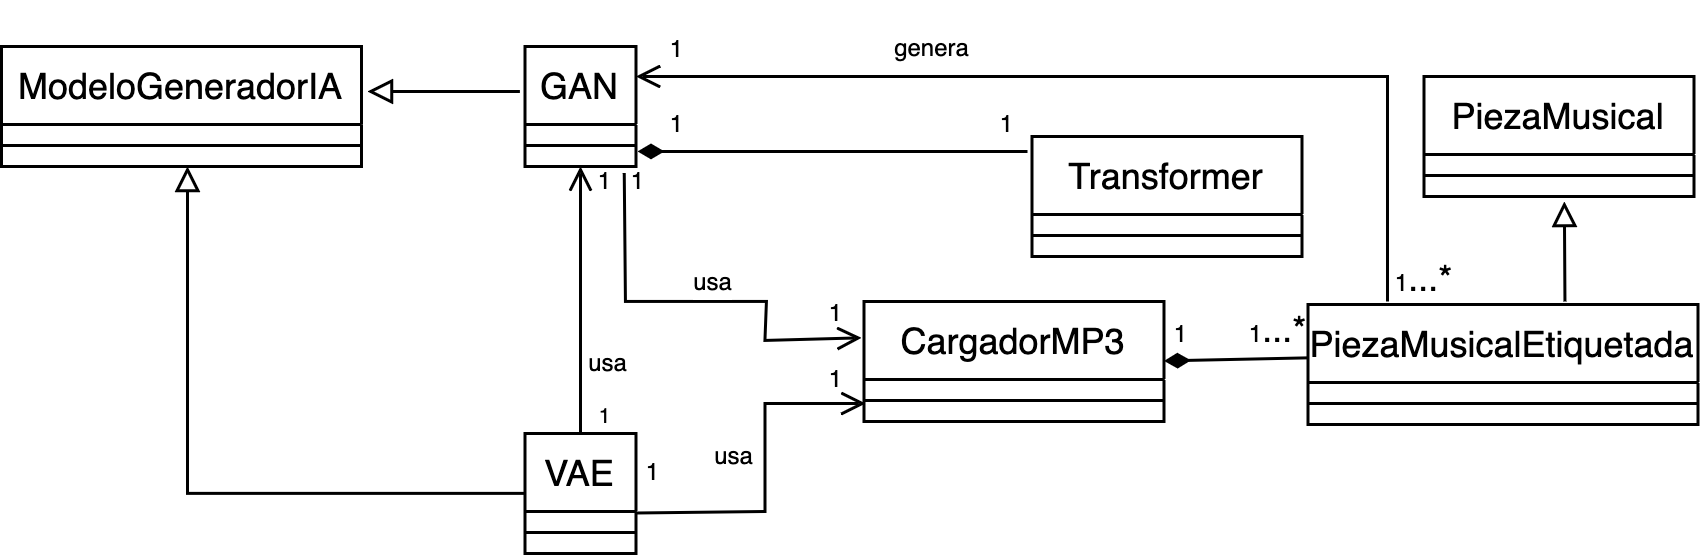
\includegraphics[width=0.9\textwidth]{images/diagrama-clases-ia.png}
    \caption{Diagrama de clases del modelo de Inteligencia Artificial.}
  \end{figure}


  \item \textbf{Diagrama de clases completo}

  \begin{figure}[H]
    \centering
    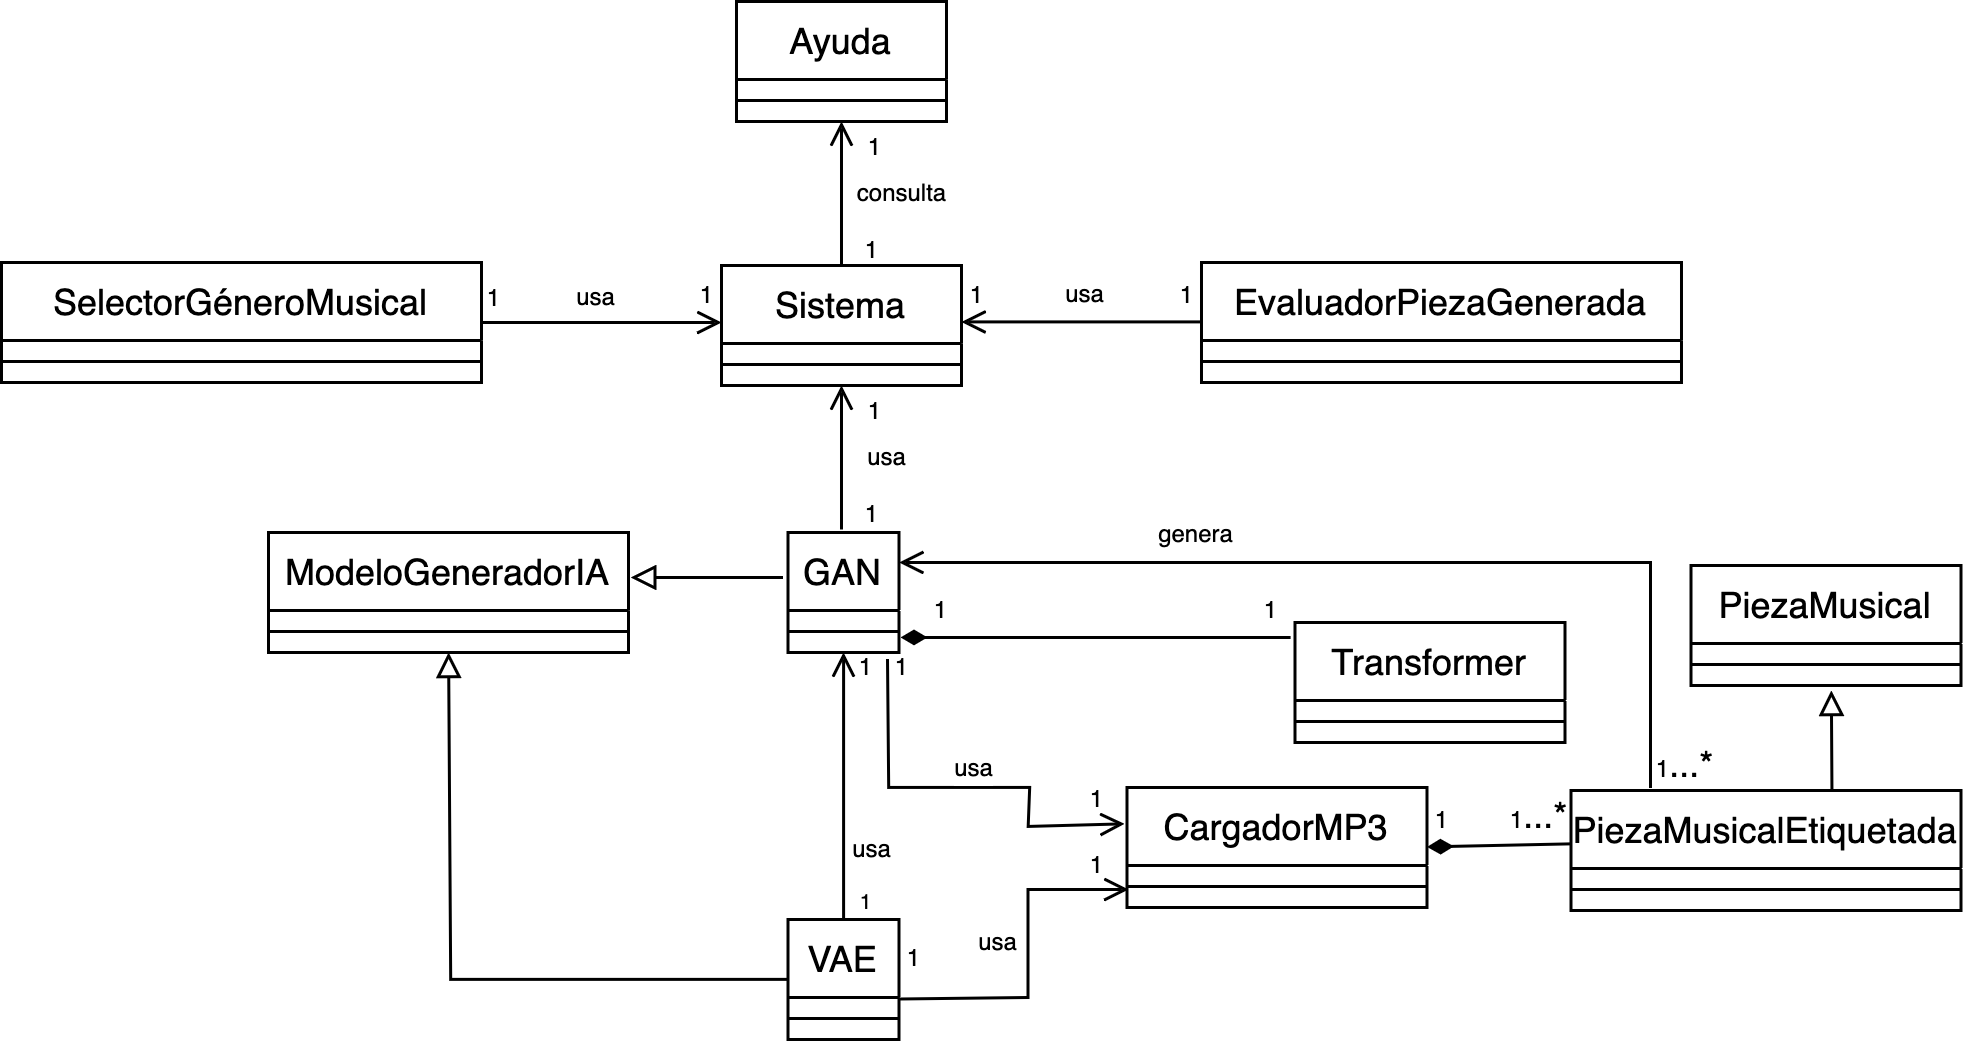
\includegraphics[width=0.9\textwidth]{images/diagrama-clases-completo.png}
    \caption{Diagrama de clases completo.}
  \end{figure}

\end{enumerate}

\subsection{Diagramas de Secuencia}

Tras la especificación del modelo de clases, el siguiente paso es crear un nuevo diagrama, en el que los dos hasta ahora mostrados, el diagrama de caso de uso y la especificación de modelo de clases, se unan y muestren una nueva visión de la información, en la que se aprecie el flujo de información entre las clases, recreando las funciones de los casos de uso, y mostrando todo esto bajo una progresión temporal. A esto se le llama Diagrama de Secuencia o Diagrama de Caso de Uso Dinámico.

En estos diagramas, la progresión temporal se despliega en el eje vertical hacia abajo, y el intercambio de datos entre clases se representa con líneas horizontales que van desde un usuario a una clase, o de una clase a otra.

Los diagramas de secuencia diseñados son los siguientes:

\begin{itemize}
    \item Creación de pieza musical.
    \item Evaluación de pieza musical.
    \item Ayuda.
\end{itemize}

Estos diagramas de secuencia dejan entrever que, en todo momento, la instanciación de objetos de clase ya se ha producido. Es decir, el sistema será un software latente e instanciable bajo demanda, que carecerá de necesidad de ser inicializado de cualquier modo.

\newpage
\subsubsection{Creación de pieza musical}

Este diagrama de secuencia representa el flujo de eventos que ocurren cuando se solicita la creación de una pieza musical.

El usuario insta al sistema, ya iniciado previamente y este le da la oportunidad de selecionar el género musical.

Tras esta selección, se produce la llamada al objeto ModeloGeneroMúsica, que devolverá una pieza musical del género requerido.

\begin{figure}[H]
  \centering
  \includesvg[width=0.9\textwidth]{images/diagrama-secuencia-generar.svg}
  \caption{Diagrama de secuencia \emph{Creación de pieza musical}.}
\end{figure}

\subsubsection{Evaluación de pieza musical}

Este diagrama de secuencia representa el flujo de eventos que ocurren cuando se emite una evaluación sobre una pieza musical generada.

El usuario insta al sistema y recorre todos los pasos a seguir para la generación de una pieza musical de un género concreto. Una vez generada, ya puede emitir su valoración. El sistema albergará dicha evaluación.

\begin{figure}[H]
  \centering
  \includesvg[width=0.9\textwidth]{images/diagrama-secuencia-eval.svg}
  \caption{Diagrama de secuencia \emph{Evaluación de pieza musical}.}
\end{figure}

\subsubsection{Consultar ayuda}

Este diagrama de secuencia representa el flujo de eventos que ocurren cuando se consulta la ayuda sobre el uso del programa.

El usuario, en cualquier momento, puede solicitar ayuda sobre el uso y funcionamiento del sistema al mismo. El sistema muestra la ayuda del programa por pantalla.

\begin{figure}[H]
  \centering
  \includesvg[width=0.5\textwidth]{images/diagrama-secuencia-ayuda.svg}
  \caption{Diagrama de secuencia \emph{Consultar ayuda}.}
\end{figure}

\subsection{Especificación de Requisitos de la Interfaz}
\label{especificacion-interfaz}
Hoy en día no se concibe un programa informático sin una interfaz gráfica de usuario.

La interfaz gráfica de usuario (GUI) brinda al usuario la capacidad de introducir y visualizar información de manera sencilla e intuitiva, y permite interaccionar con una aplicación de manera más amigable.

Además de esto, las GUI son una parte fundamental en una sociedad en que la imagen externa se antepone a la potencialidad o valor oculto tras esa máscara. De ahí la expresión: ``se mete por los ojos''. Algo que ``entra por los ojos'' es algo que cala de tal manera que tiene más probabilidad de ser aceptado que lo que no nos parece atractivo.

La GUI también permite el acceso a la informática a personas cuyas discapacidades dificultan o impiden el manejo de un antiguo programa de consola, o también da acceso a un colectivo social como es el colectivo infantil, al que permanecer delante de algo que no estimula su atención le resulta muy difícil.

Puesto que esta aplicación va orientada al uso por parte del mayor número de usuarios, con perfiles personales y profesionales distintos, la interfaz gráfica ha de ser lo más sencilla y amigable posible.

El programa se compondrá de una única ventana principal, cuyo contenido será:

\begin{itemize}
    \item Una lista de géneros musicales para seleccionar.
    \item Un botón para instar la creación de una pieza musical del género seleccionado.
    \item Un botón para dirigirse a la zona de ayuda de la ventana.
    \item Un pequeño panel que se activará cuando se recepciones el fichero con la pieza musical y que permitirá al usuario emitir una valoración entre 1 y 10 de la fidelidad de dicha pieza con el género solicitado.
\end{itemize}
\input{UML/diseño-de-clases}

\subsection{Diagrama de Paquetes}

La complejidad y tamaño de un diagrama de clases de un sistema puede llevar que la aprehensión del mismo sea compleja y difusa.

En la programación estructurada, la manera de crear un nivel más alto de abstracción es la creación de las funciones. Pero en la programación orientada a objetos, donde los datos y el procesamiento no se presentan por separado, la única manera de realizar un diagrama más inteligible y abordable, así como más sencillo de entender es el diagrama de paquetes.

Un paquete es una estructura superior, mediante la cual se agrupan varias clases, atendiendo a un criterio de empaquetamiento. El criterio usado para crear el diagrama de paquetes de este proyecto es el desempeño. Así, todas las clases utilizadas para un misma finalidad estarán agrupadas bajo un mismo paquete.

Los paquetes que se pueden extraer de la sección ``Diseño de clases'' \ref{diseño-clases} son los siguientes:

\begin{itemize}
    \item Aplicación.
    \item CargadorDataset.
    \item ModelosIA.
\end{itemize}

No existirá jerarquía entre paquetes, por lo tanto, ningún paquete contendrá a uno o varios otros.

\subsubsection{Paquete Aplicación}
Este paquete contiene las clases encargadas de conformar una aplicación informática de cara al usuario. 

Las clases contenidas son:

\begin{itemize}
  \item Sistema.
  \item SelectorGéneroMusical.
  \item EvaluadorPiezaGenerada.
  \item Ayuda.
\end{itemize}

La clase \emph{Sistema} y por ende, este paquete, verán al modelo de Inteligencia Artificial ya compilado como recurso.

\subsubsection{Paquete ModelosIA}

Este otro paquete es el encargado de contener todas las clases que intervienen en la conformación de un modelo de Inteligencia Artificial y que dará lugar a los objetos de sendos modelos utilizados en este trabajo.

La lista de clases que se pueden encontrar en este paquete son:
\begin{itemize}
  \item modeloGeneradorIA.
  \item VAE.
  \item GAN.
  \item Transformer.
\end{itemize}


\subsubsection{Paquete CargadorDataset}

Las clases que están contenidas en este paquete van orientadas al manejo del \emph{Dataset} y la abstracción de las piezas musicales en él contenidas.

Las clases que conforman este paquete son:
\begin{itemize}
  \item PiezaMusical.
  \item PiezaMusicalEtiquetada.
  \item CargadorMP3.
  \item ScriptEntrenamiento.
\end{itemize}

Se hace un especial hincapié en la clase \emph{ScriptEntrenamiento}, que si bien no está colocada en este paquete de manera trivial, pues sirve para manejar el \emph{Dataset}, también controla y gestiona todo el proceso de entrenamiento de los modelos y es la pieza central de todo el proceso previa puesta en producción, que se hace para generarlos.


\subsubsection{Diagrama general de paquetes}

\begin{figure}[H]
  \centering
  \includesvg[width=0.4\textwidth]{images/diagrama-paquetes.svg}
  \caption{Diagrama general de paquetes.}
\end{figure}

\input{UML/diseño-de-la-interfaz}

\chapter{Resultados y Análisis}

Tal y como se puede apreciar en el diagrama de flujo de CRISP-ML(Q)\ref{fig:crispml-q-diagram}, la Preparación de los datos es un paso crucial en el desarrollo. Tal es así, que son 4 las tareas definidas en Scrum para ello:
\begin{itemize}
    \item PD-1: normalizar y codificar variables.
    \item PD-2: manejar valoras atípicos y nulos.
    \item PD-3: definir proporción de sepación de datos.
    \item PD-4: verificar balanceo de clases.
\end{itemize}

Las dos últimas, PD-3 y PD-4, inferirán de manera capital en la calidad de los resultados; pero las dos primeras son las que harán que el entrenamiento se pueda llevar a cabo o no, las que harán que la programación discurra por unos derroteros u otros, dependiendo del nivel de ``suciedad'' o divergencia que se encuentre en los datos y del nivel de homogeneidad que se demande.

Así pues, se procede a realizar un análisis exploratorio de datos, en aras de conocer amortiguar en la medida de lo posible, todas las dificultades que puedan encontrarse.

\section{Análisis Exploratorio de Datos (EDA)}

El análisis exploratorio de datos constituye un paso esencial en este estudio sobre la generación de música personalizada mediante modelos generativos adversariales (GANs). Se han utilizado tres conjuntos de datos principales: \textbf{FMA (Free Music Archive)}, \textbf{Million Song Dataset} y \textbf{MTG-Jamendo}, los cuales contienen una amplia diversidad de géneros y metadatos relacionados.

\subsection{Distribución de los datos}
Se ha trabajado con un total de \textbf{176,500 pistas de audio}, distribuidas de la siguiente manera:
\begin{itemize}
\item \textbf{FMA Large}: 106,000 pistas, 161 géneros.
\item \textbf{Million Song Dataset}: 25,000 pistas, 15 géneros.
\item \textbf{MTG-Jamendo Dataset}: 50,000 pistas, 190 géneros.
\end{itemize}

Para garantizar la coherencia del conjunto de datos:
\begin{itemize}
\item Se han filtrado archivos corruptos o incompletos.
\item Se ha unificado la estructura de etiquetas de género.
\item Se ha establecido una duración uniforme de \textbf{30 segundos} para cada clip de audio. (Esta duración se podrá ver modificada según sea la experiencia durante el entrenamiento. La duración más conservadora elegible serían 25 segudos, pues están asegurados en todas las muestras de los 3 conjuntos).
\end{itemize}

\subsection{Distribución de géneros}
Los cinco géneros musicales más representados en la base de datos son:
\begin{enumerate}
\item Rock (35,200 pistas)
\item Pop (30,100 pistas)
\item Jazz (22,800 pistas)
\item Hip-Hop (19,500 pistas)
\item Electrónica (17,900 pistas)
\end{enumerate}

Se realizaá un análisis espectral de los archivos de audio mediante \textbf{MFCCs (Mel-Frequency Cepstral Coefficients)} y \textbf{espectrogramas de corto tiempo (STFT)}. Esto permitió visualizar la distribución de frecuencias y la evolución de los patrones tonales en los diferentes géneros.

\section{Evaluación}

\subsection{Evaluación de modelos}
Se comparaán los dos enfoques principales para la generación de música:
\begin{enumerate}
\item \textbf{VAE (Variational Autoencoder)}: utilizado como línea base para evaluar la capacidad de modelado latente de los datos musicales.
\item \textbf{GAN + Transformer}: modelo basado en redes generativas adversariales con un componente de atención para mejorar la coherencia musical.
\end{enumerate}

\subsection{Métricas de Evaluación}
Se llevarán a cabo diversas métricas cuantitativas y cualitativas para evaluar la calidad de la música generada:
\begin{itemize}
\item \textbf{FID (Fréchet Inception Distance)}: Evalúa la similitud estadística entre las pistas generadas y las reales.
\item \textbf{IS (Inception Score)}: Mide la diversidad de las muestras generadas.
\item \textbf{Perplejidad Espectral}: Determina la coherencia en la estructura armónica y melódica.
\item \textbf{Evaluación subjetiva con oyentes humanos}: Se hará una encuesta al mayor número de participantes posibles, los cuales calificarán la naturalidad y coherencia de las piezas generadas en una escala de 1 a 10.
\end{itemize}

\subsection{Resultados}

En estos momentos, los dos modelos se encuentran bajo desarrollo.

Se ha conseguido extraer el espectrograma con \emph{sampling} de 10 milisegundos de más de un 70\% del dataset y se ha focalizado el entremaiento previo en 5 géneros:
\begin{itemize}
    \item hip-hop
    \item pop
    \item rock
    \item jazz
    \item blues
\end{itemize}

Los entrenamientos en estos momentos no se llegan a completar por fallos de código fuente, que se están subsanando día a día.

\cleardoublepage
\phantomsection

% \printglossary[type=\acronymtype]
% \printglossary

\appendix
%% APÉNDIZES

% Escribe cada apéndize como si fuera un capítulo más.

\chapter{Apéndize A}
\label{apendize-a}

\chapter{Apéndize B}
\label{apendize-b}

\chapter{Lista de librerías y versiones}

\begin{table}[h]
    \caption{Lista de paquetes y versiones}
    \centering
    \resizebox{\textwidth}{!}{%
    \begin{tabular}{llp{1.5cm}llp{1.5cm}llp{1.5cm}ll}
        \toprule
        \textbf{Paquete} & \textbf{Versión} & & \textbf{Paquete} & \textbf{Versión} & & \textbf{Paquete} & \textbf{Versión} & & \textbf{Paquete} & \textbf{Versión} \\
        \midrule

        absl-py & 2.1.0 & & aiohappyeyeballs & 2.6.1 & & aiohttp & 3.11.14 & & aiosignal & 1.3.2 \\
        anyio & 4.7.0 & & argon2-cffi & 23.1.0 & & argon2-cffi-bindings & 21.2.0 & & arrow & 1.3.0 \\
        asttokens & 3.0.0 & & astunparse & 1.6.3 & & async-lru & 2.0.4 & & attrs & 24.3.0 \\
        audioread & 3.0.1 & & babel & 2.16.0 & & beautifulsoup4 & 4.12.3 & & bleach & 6.2.0 \\
        certifi & 2024.12.14 & & cffi & 1.17.1 & & charset-normalizer & 3.4.0 & & comm & 0.2.2 \\
        contourpy & 1.3.1 & & cycler & 0.12.1 & & debugpy & 1.8.11 & & decorator & 5.1.1 \\
        defusedxml & 0.7.1 & & dotenv & 0.9.9 & & executing & 2.1.0 & & fastjsonschema & 2.21.1 \\
        filelock & 3.16.1 & & flatbuffers & 24.3.25 & & fonttools & 4.55.3 & & fqdn & 1.5.1 \\
        frozenlist & 1.5.0 & & fsspec & 2024.12.0 & & gast & 0.6.0 & & google-pasta & 0.2.0 \\
        grpcio & 1.68.1 & & h11 & 0.14.0 & & h5py & 3.12.1 & & httpcore & 1.0.7 \\
        httpx & 0.28.1 & & idna & 3.10 & & ipykernel & 6.29.5 & & ipython & 8.31.0 \\
        ipywidgets & 8.1.5 & & isoduration & 20.11.0 & & jedi & 0.19.2 & & Jinja2 & 3.1.4 \\
        joblib & 1.4.2 & & json5 & 0.10.0 & & jsonpointer & 3.0.0 & & jsonschema & 4.23.0 \\
        jsonschema-specifications & 2024.10.1 & & jupyter & 1.1.1 & & jupyter\_client & 8.6.3 & & jupyter-console & 6.6.3 \\
        jupyter\_core & 5.7.2 & & jupyter-events & 0.11.0 & & jupyter-lsp & 2.2.5 & & jupyter\_server & 2.15.0 \\
        jupyter\_server\_terminals & 0.5.3 & & jupyterlab & 4.3.4 & & jupyterlab\_pygments & 0.3.0 & & jupyterlab\_server & 2.27.3 \\
        jupyterlab\_widgets & 3.0.13 & & kaggle & 1.6.17 & & keras & 3.7.0 & & kiwisolver & 1.4.7 \\
        lazy\_loader & 0.4 & & libclang & 18.1.1 & & librosa & 0.10.2.post1 & & lightning-utilities & 0.14.2 \\
        llvmlite & 0.44.0 & & Markdown & 3.7 & & markdown-it-py & 3.0.0 & & MarkupSafe & 3.0.2 \\
        matplotlib & 3.10.0 & & matplotlib-inline & 0.1.7 & & mdurl & 0.1.2 & & mistune & 3.0.2 \\
        ml-dtypes & 0.3.2 & & mpmath & 1.3.0 & & msgpack & 1.1.0 & & multidict & 6.2.0 \\
        mutagen & 1.47.0 & & namex & 0.0.8 & & nbclient & 0.10.2 & & nbconvert & 7.16.4 \\
        nbformat & 5.10.4 & & nest-asyncio & 1.6.0 & & networkx & 3.4.2 & & notebook & 7.3.1 \\
        notebook\_shim & 0.2.4 & & numba & 0.61.0 & & numpy & 1.26.4 & & nvidia-cublas-cu12 & 12.4.5.8 \\
        nvidia-cuda-cupti-cu12 & 12.4.127 & & nvidia-cuda-nvrtc-cu12 & 12.4.127 & & nvidia-cuda-runtime-cu12 & 12.4.127 & & nvidia-cudnn-cu12 & 9.1.0.70 \\
        nvidia-cufft-cu12 & 11.2.1.3 & & nvidia-curand-cu12 & 10.3.5.147 & & nvidia-cusolver-cu12 & 11.6.1.9 & & nvidia-cusparse-cu12 & 12.3.1.170 \\
        nvidia-cusparselt-cu12 & 0.6.2 & & nvidia-nccl-cu12 & 2.21.5 & & nvidia-nvjitlink-cu12 & 12.4.127 & & nvidia-nvtx-cu12 & 12.4.127 \\
        opt\_einsum & 3.4.0 & & optree & 0.13.1 & & overrides & 7.7.0 & & packaging & 24.2 \\
        pandas & 2.2.3 & & pandocfilters & 1.5.1 & & parso & 0.8.4 & & pexpect & 4.9.0 \\
        pillow & 11.0.0 & & pip & 25.0.1 & & platformdirs & 4.3.6 & & pooch & 1.8.2 \\
        prometheus\_client & 0.21.1 & & prompt\_toolkit & 3.0.48 & & propcache & 0.3.1 & & protobuf & 4.25.5 \\
        psutil & 6.1.1 & & ptyprocess & 0.7.0 & & pure\_eval & 0.2.3 & & pycparser & 2.22 \\
        pydot & 3.0.4 & & pydub & 0.25.1 & & Pygments & 2.18.0 & & pyparsing & 3.2.0 \\
        python-dateutil & 2.9.0.post0 & & python-dotenv & 1.0.1 & & python-json-logger & 3.2.1 & & pytorch-lightning & 2.5.1 \\
        pytz & 2024.2 & & PyYAML & 6.0.2 & & pyzmq & 26.2.0 & & referencing & 0.35.1 \\
        requests & 2.32.3 & & rfc3339-validator & 0.1.4 & & rfc3986-validator & 0.1.1 & & rich & 13.9.4 \\
        rpds-py & 0.22.3 & & scikit-learn & 1.6.0 & & scipy & 1.14.1 & & seaborn & 0.13.2 \\
        Send2Trash & 1.8.3 & & setuptools & 75.6.0 & & six & 1.17.0 & & slugify & 0.0.1 \\
        sniffio & 1.3.1 & & soundfile & 0.13.1 & & soupsieve & 2.6 & & soxr & 0.5.0.post1 \\
        stack-data & 0.6.3 & & sympy & 1.13.1 & & tensorboard & 2.16.2 & & tensorboard-data-server & 0.7.2 \\
        tensorflow & 2.16.1 & & termcolor & 2.5.0 & & terminado & 0.18.1 & & threadpoolctl & 3.5.0 \\
        tinycss2 & 1.4.0 & & torch & 2.6.0 & & torchaudio & 2.6.0 & & torchmetrics & 1.7.0 \\
        torchvision & 0.21.0 & & tornado & 6.4.2 & & tqdm & 4.67.1 & & traitlets & 5.14.3 \\
        triton & 3.2.0 & & types-python-dateutil & 2.9.0.20241206 & & typing\_extensions & 4.12.2 & & tzdata & 2024.2 \\
        uri-template & 1.3.0 & & urllib3 & 2.2.3 & & wcwidth & 0.2.13 & & webcolors & 24.11.1 \\
        webencodings & 0.5.1 & & websocket-client & 1.8.0 & & Werkzeug & 3.1.3 & & wheel & 0.45.1 \\
        widgetsnbextension & 4.0.13 & & wrapt & 1.17.0 & & yarl & 1.18.3 & &  &  \\
        \bottomrule
    \end{tabular}
    }
    \label{apendice-a:paquetes}
\end{table}


\begin{singlespace}
\begin{footnotesize}
\begin{twocolumn}
\nocite{*}
\bibdata{bibliografia}
\bibliographystyle{apa}
\bibliography{bibliografia}
\addcontentsline{toc}{chapter}{Bibliografía}
\end{twocolumn}
\end{footnotesize}
\end{singlespace}

\end{document}
